% interactnlmsample.tex
% v1.05 - August 2017

\documentclass[dvipdfmx]{interact}
\usepackage{epstopdf}
\usepackage[caption=false]{subfig}

\usepackage{graphics,amsmath,amssymb,bm,float,cases}
\usepackage{here}
\usepackage{comment}
\usepackage{url}
\usepackage{layout}
\usepackage{tabularx}
\usepackage{algorithm}
\usepackage{algorithmic}
\usepackage{xcolor}
\usepackage{multirow}


\usepackage[numbers,sort&compress]{natbib}% Citation support using natbib.sty
\bibpunct[, ]{[}{]}{,}{n}{,}{,}% Citation support using natbib.sty
\renewcommand\bibfont{\fontsize{10}{12}\selectfont}% Bibliography support using natbib.sty
\makeatletter% @ becomes a letter
\def\NAT@def@citea{\def\@citea{\NAT@separator}}% Suppress spaces between citations using natbib.sty
\makeatother% @ becomes a symbol again

\theoremstyle{plain}% Theorem-like structures provided by amsthm.sty
\newtheorem{theorem}{Theorem}[section]
\newtheorem{lemma}[theorem]{Lemma}
\newtheorem{corollary}[theorem]{Corollary}
\newtheorem{proposition}[theorem]{Proposition}
\newtheorem{assumption}{Assumption}

\theoremstyle{definition}
\newtheorem{definition}[theorem]{Definition}
\newtheorem{example}[theorem]{Example}

\theoremstyle{remark}
\newtheorem{remark}{Remark}
\newtheorem{notation}{Notation}


% \newcommand{\Figref}[1]{Figure \ref{#1}}
% \newcommand{\Tabref}[1]{Table \ref{#1}}
% \newcommand{\Eqref}[1]{(Equation \ref{#1})}
% \newcommand{\Secref}[1]{Section \ref{#1}}
% \newcommand{\Theoref}[1]{Theorem \ref{#1}}
\DeclareGraphicsExtensions{.eps,.pdf,.png,.jpg}
\newcommand{\Tabref}[1]{{Table~\ref{#1}}}
\newcommand{\Eqref}[1]{Eq.~(\ref{#1})}
\newcommand{\Figref}[1]{{Fig.~\ref{#1}}}

\begin{document}

\articletype{ARTICLE TEMPLATE}% Specify the article type or omit as appropriate

\title{Probabilistic Multi-Agent Pose Graph Filtering on SE(3) \\ via Distributed ADMM and Stein Particle Gradient Descent}

\author{
\name{Tomoki Arita\textsuperscript{a} and Toru Namerikawa\textsuperscript{b}\thanks{CONTACT Tomoki Arita. Email: arita.tomoki@keio.jp, Toru Namerikawa. Email: namerikawa@sd.keio.ac.jp}}
\affil{\textsuperscript{a} School of Integrated Design Engineering, Keio University, Kanagawa, Japan\\
	\textsuperscript{b} Department of System Design Engineering, Keio University, Kanagawa, Japan}
}

\maketitle

\begin{abstract}
    This paper proposes a novel distributed probabilistic pose graph filtering framework on SE(3). It integrates ADMM with Stein Variational Gradient Descent (SVGD) to address multi-modal, non-Gaussian posteriors in multi-robot SLAM.
    We reformulate pose graph filtering as Bayesian posterior estimation on SE(3) using particles. The consistency requirement, minimizing KL divergence, is cast into an augmented Lagrangian and decomposed via ADMM. Agents perform local SVGD updates and consensus steps, communicating only summary statistics.
    The proposed method (i) maintains multiple hypotheses for ambiguous loop closures, (ii) reduces communication by exchanging only Lagrange multipliers and particle summaries, and (iii) handles SE(3) nonlinearity. Convergence is proven under standard ADMM conditions, and KL minimization is validated.
    Simulations demonstrate real-time convergence, outlier robustness, and accurate posterior approximation.
\end{abstract}

\begin{keywords}
Probabilistic pose graph filtering; SE(3); ADMM; Stein Variational Gradient Descent; Multi-robot SLAM
\end{keywords}

\section{序論}

\subsection{共有視野保証の重要性と背景}

マルチロボットシステムでは,各ロボットがセンサ情報や視界を共有することにより,監視・捜索・協調輸送などのタスクを効率的に遂行できることが知られている.
特にカメラを用いた視覚協調の場合,各ロボットの共有視野(Common Field-of-View, CoFoV)が不可欠である.例えば,複数ドローンが異なる角度から同一対象を観測できることや,通信の見通し線(LOS)維持が求められる\cite{Panagou2017}.

マルチエージェントVSLAM(Visual Simultaneous Localization and Mapping)においては,各エージェントが撮影した画像から抽出される局所特徴に基づき自己局在を行い,エージェント間で特徴マッチングにより相対位置を推定する.従来のORBやSIFTに代わり,SuperPointのような学習型局所特徴検出・記述器\cite{DeTone2018}や,NetVLADによるグローバル記述子\cite{Arandjelovic2016}が高いロバスト性を示し,ループ検出やキーフレームマッチングに貢献している.

画像特徴量のマッチングを成功させるためには,各エージェントが共通のランドマークを観測できるよう,カメラの視野錐台の幾何学的重複が必要である.視野重複が存在すれば,エージェント間でのループ検出が可能となり,その結果として各ロボットの地図統合が実現される\cite{Zhang2022}.しかし,ロボットは視野角が限られているため,視界共有を保証するための制御技術の開発が急務である.

\red{モチベーション:CoVINSではsuperpoint特徴量などの画像特徴量のマッチングにより、自己位置推定に関する最適化問題のfactorを得ている。特徴量をマッチングするにはエージェントの視野錐台が重なっている必要がある。single agent問題に関してはstereo cameraの相対位置をconstかつgivenとして最適化問題に組み込み、multi agent問題に関しては視野錐台のoverrideは不可知であるために画像全体特徴量の類似度の一致などによってpassiveなevent trigger型としてアルゴリズムが構築されている。しかし、agent1とagent2が視野錐台を交差させ続けるための制御則(CBF等)に基づいてactive perceptionを行う場合、multi agentの自己位置推定においてinter-agentな特徴量のマッチング及び推定問題はエージェントをまたいだカメラ間の相対位置をgiven, もしくは最適化すべき双対変数として複数のエージェント位置を同時最適化できるはずである。さらに、active perceptionの枠組みで考えれば、CBFを用いた最適制御問題と自己位置推定問題も同一の目的関数の最小化問題として扱うことができるはずである。  
上記の仮定から、本セミナーではその手始めとして,代表的なCoVINSであるUAVを対象として、視野錐台を交差させ続けるための分散型CBF手法を提案する。}

\begin{figure}[htbp]
\centering
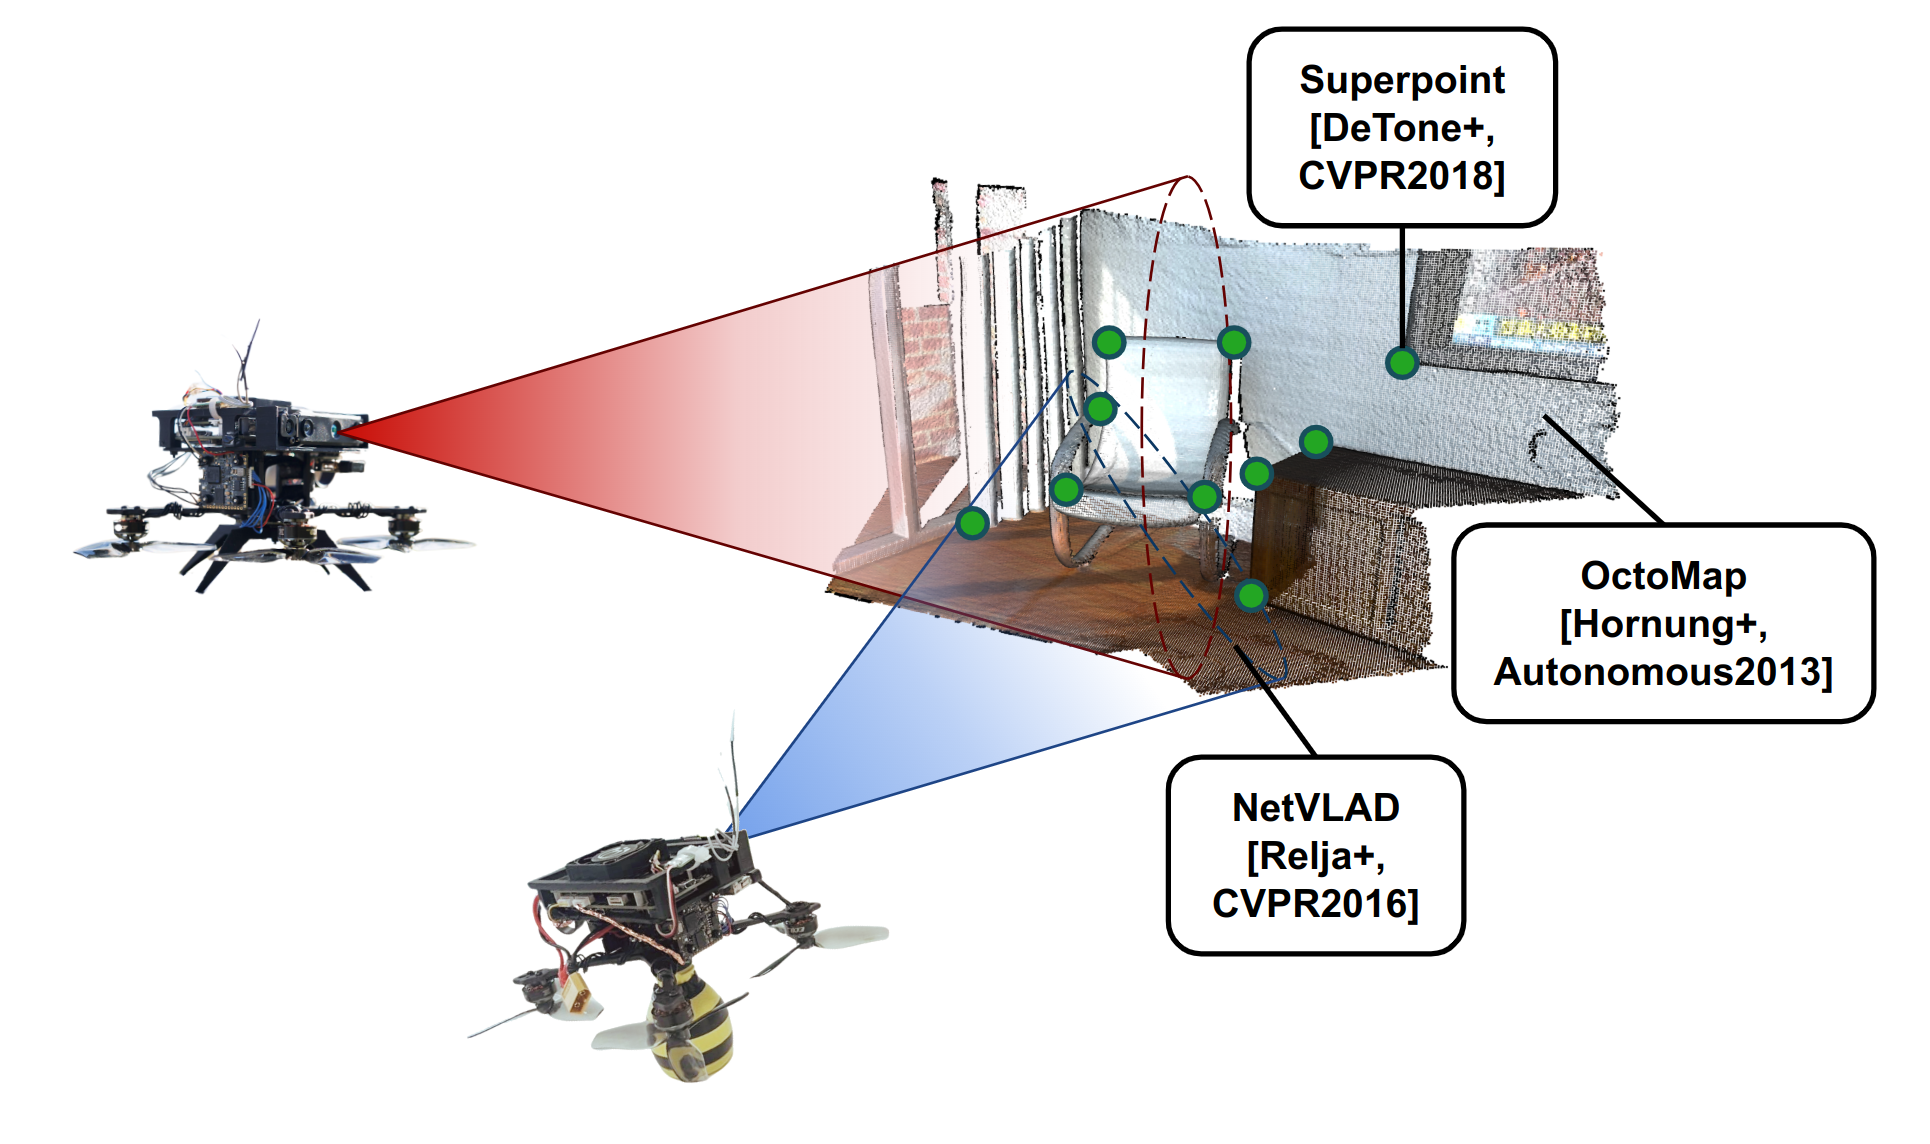
\includegraphics[width=0.8\linewidth]{fig/covins.png}
\caption{COVINSの構成}
\label{fig:covins}
\end{figure}
\subsection{既存研究の課題}

従来はポテンシャル場やMPC(Model Predictive Control)を用いた手法が提案され,局所的な視界制約下での隊列制御やセンサグラフの連結性維持に取り組まれてきた\cite{Sabattini2013}.一方で,制御バリア関数(Control Barrier Function, CBF)を用いた手法は,制約違反を防ぎながらリアルタイムに最適な制御入力を計算できるため,有力な候補となる\cite{Capelli2020}.

しかし,現状の協調SLAMは,キーフレームの受動的な共有と画像類似度評価に依存しており,視野重複が偶発的に発生しなければマップ統合が成立しないリスクがある.また,多数のロボットを対象とする場合,中央集権的な制御は通信負荷や計算量の面で現実的ではなく,各エージェントが局所的に計算し,限定的な通信で連携する分散アルゴリズムの設計が必要である.

従来の視野維持手法は,対象が視野内にあるか否かを決定論的に評価するに留まっていたが,センサの観測不確実性を十分に取り入れていなかった\cite{Panagou2012}.また,従来の多くの視野制約付き制御手法は,単純な動力学モデル(例:Dubins車両やクアッドロータの水平姿勢維持)に基づいており,非ホロノミックなダイナミクスを明示的に考慮していなかった\cite{Dias2016}.

\subsection{本研究の貢献}

本研究では,SE(3)上における協調自己位置推定のための視野共有を保証する分散型CBF手法を提案する.本研究の主な貢献は以下の通りである.

\begin{itemize}
\item SE(3)における共有視野保証を実現する.従来のステレオ視やリーダーフォロワ形式による視野制御は,ロボット間の相対配置を幾何学的に制約するに留まっていたが,本手法は3次元空間におけるエージェント全体の姿勢・位置を統合的に制御する枠組みを提供する.

\item 特徴点に基づく確率的可視性制約とCBFの適用を行う.本研究では,各エージェントが観測する特徴点に基づき,その可視性を確率的に評価した上で,CBFに組み込み,常時高い確率で共有視野が確保されるよう制御入力を設計する.これにより,センサノイズ等による不確実性下でも安全な視野維持が可能となる.

\item 非ホロノミックなドローンダイナミクスへの対応と分散最適化を実現する.本研究では,機体の並進および回転運動を同時に考慮するSE(3)上の非ホロノミックドローンモデルに対して,高次制約も扱える高次制御バリア関数(HOCBF)を導入し,各エージェントが局所的な情報交換を通じて分散最適化アルゴリズム(PDMM等)により制御解を求める枠組みを提案する\cite{Lv2024}.これにより,リアルタイム性とスケーラビリティの両立を実現する.
\end{itemize}

\subsection{論文構成}

本論文の構成は以下の通りである.第2章ではCBFの基本概念と高次CBFについて説明する.第3章では問題設定とシステムモデルについて述べる.第4章では共有視野のためのCBFを提案し,第5章では二次系システムのための高次CBFを導入する.第6章ではシミュレーション結果を示し,第7章で結論と今後の課題について述べる.

\begin{figure}[htbp]
\centering
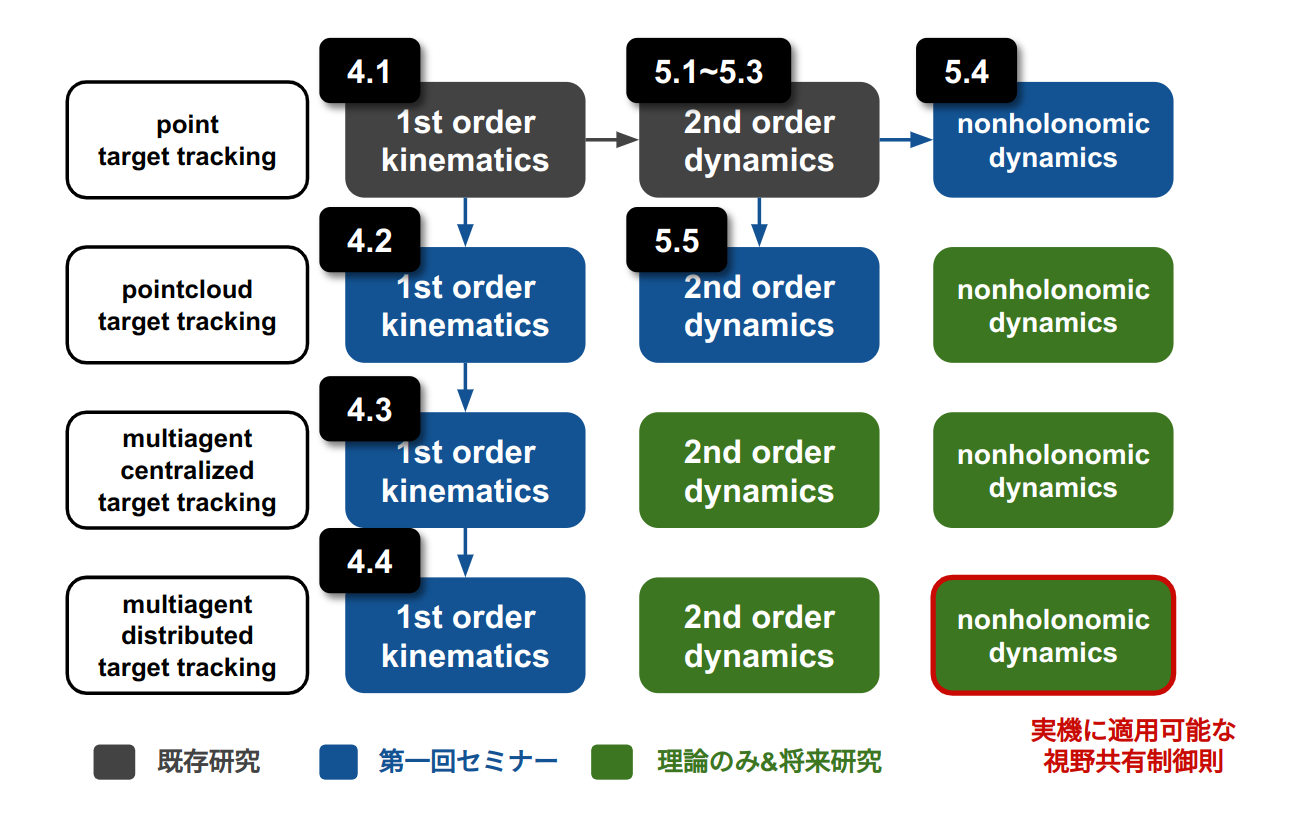
\includegraphics[width=0.8\linewidth]{fig/progress.png}
\caption{第一回セミナーの内容と本研究の貢献点}
\label{fig:progress}
\end{figure}
% \section{\textbf{準備:制御バリア関数}}
\section{準備:制御バリア関数}

本章では,本研究の基礎となる制御バリア関数(Control Barrier Function, CBF)の基本概念と高次制御バリア関数(High Order Control Barrier Function, HOCBF)について説明する.

\subsection{CBFの基本概念}

CBFは,システム状態がある安全集合内に留まることを保証するためのLyapunov関数に類似した概念である.以下では,CBFの基本的な定義と性質について述べる.

連続時間の制御アフィンシステムを考える:
\begin{equation}
\begin{aligned}
\dot{\mathbf{x}} = f(\mathbf{x}) + g(\mathbf{x})\mathbf{u}
\label{eq:control_affine}
\end{aligned}
\end{equation}
ここで,$\mathbf{x} \in \mathbb{R}^n$は状態,$\mathbf{u} \in \mathbb{R}^m$は制御入力,$f: \mathbb{R}^n \rightarrow \mathbb{R}^n$と$g: \mathbb{R}^n \rightarrow \mathbb{R}^{n \times m}$は局所Lipschitz連続な関数である.

安全集合$\mathcal{C}$を以下のように定義する:
\begin{equation}
\begin{aligned}
\mathcal{C} = \{\mathbf{x} \in \mathbb{R}^n : h(\mathbf{x}) \geq 0\}
\label{eq:safe_set}
\end{aligned}
\end{equation}
ここで,$h: \mathbb{R}^n \rightarrow \mathbb{R}$は連続微分可能な関数である.

\begin{dfn}[制御バリア関数]
関数$h: \mathbb{R}^n \rightarrow \mathbb{R}$が連続微分可能であり,その勾配$\nabla h(\mathbf{x})$が$\mathcal{C}$上でゼロにならないとする.このとき,$h$が制御バリア関数であるとは,ある拡張クラス$\mathcal{K}_{\infty}$関数$\alpha$が存在して,任意の$\mathbf{x} \in \mathcal{C}$に対して以下の条件を満たす制御入力$\mathbf{u} \in \mathbb{R}^m$が存在することである:
\begin{equation}
\begin{aligned}
L_f h(\mathbf{x}) + L_g h(\mathbf{x})\mathbf{u} + \alpha(h(\mathbf{x})) \geq 0
\label{eq:cbf_condition}
\end{aligned}
\end{equation}
ここで,$L_f h(\mathbf{x}) = \nabla h(\mathbf{x})^T f(\mathbf{x})$と$L_g h(\mathbf{x}) = \nabla h(\mathbf{x})^T g(\mathbf{x})$はそれぞれ$h$の$f$と$g$に関するLie微分である.
\end{dfn}

CBFの重要な性質は,\Eqref{eq:cbf_condition}を満たす任意の制御入力$\mathbf{u}$を用いると,安全集合$\mathcal{C}$が前方不変となることである.つまり,初期状態$\mathbf{x}(0) \in \mathcal{C}$に対して,任意の時刻$t \geq 0$において$\mathbf{x}(t) \in \mathcal{C}$が保証される.

実際の制御設計では,CBF制約を満たしつつ,制御目標を達成するための最適制御入力を求めることが多い.これは以下のような二次計画問題(Quadratic Programming, QP)として定式化できる:
\begin{equation}
\begin{aligned}
\mathbf{u}^* &= \underset{\mathbf{u} \in \mathbb{R}^m}{\text{argmin}} \:\: \|\mathbf{u} - \mathbf{u}_{\text{nom}}\|^2 \\
\text{s.t.} & \:\: L_f h(\mathbf{x}) + L_g h(\mathbf{x})\mathbf{u} + \alpha(h(\mathbf{x})) \geq 0
\label{eq:cbf_qp}
\end{aligned}
\end{equation}
ここで,$\mathbf{u}_{\text{nom}}$は安全制約を考慮しない場合の公称制御入力である.

\subsection{高次制御バリア関数}

従来のCBFは制約関数の相対次数が1であることを仮定していたが,多くの実システムでは安全制約が高次微分に依存するため,高次制御バリア関数(HOCBF)が必要となる.

関数$h(\mathbf{x})$の相対次数が$r > 1$の場合,以下のように補助関数の連鎖を定義する:
\begin{equation}
\begin{aligned}
\psi_0(\mathbf{x}) &= h(\mathbf{x}) \\
\psi_1(\mathbf{x}) &= \dot{\psi}_0(\mathbf{x}) + \alpha_1(\psi_0(\mathbf{x})) \\
\psi_2(\mathbf{x}) &= \dot{\psi}_1(\mathbf{x}) + \alpha_2(\psi_1(\mathbf{x})) \\
&\vdots \\
\psi_{r-1}(\mathbf{x}) &= \dot{\psi}_{r-2}(\mathbf{x}) + \alpha_{r-1}(\psi_{r-2}(\mathbf{x}))
\label{eq:hocbf_psi}
\end{aligned}
\end{equation}
ここで,$\alpha_i$($i = 1, 2, \ldots, r-1$)は拡張クラス$\mathcal{K}$関数である.

\begin{dfn}[高次制御バリア関数]
関数$h: \mathbb{R}^n \rightarrow \mathbb{R}$が$r$回連続微分可能であり,その相対次数が$r$であるとする.このとき,$h$が高次制御バリア関数であるとは,拡張クラス$\mathcal{K}$関数$\alpha_1, \alpha_2, \ldots, \alpha_r$が存在して,以下の条件を満たすことである:
\begin{equation}
\begin{aligned}
L_f^r h(\mathbf{x}) + L_g L_f^{r-1} h(\mathbf{x})\mathbf{u} + \alpha_r(\psi_{r-1}(\mathbf{x})) \geq 0
\label{eq:hocbf_condition}
\end{aligned}
\end{equation}
ここで,$L_f^r h(\mathbf{x})$は$h$の$f$に関する$r$次のLie微分,$L_g L_f^{r-1} h(\mathbf{x})$は$L_f^{r-1} h(\mathbf{x})$の$g$に関するLie微分である.
\end{dfn}

HOCBFを用いた制御設計では,\Eqref{eq:hocbf_condition}の制約を満たす制御入力を求めることで,安全集合$\mathcal{C}$の前方不変性を保証できる.これは以下のようなQP問題として定式化できる:
\begin{equation}
\begin{aligned}
    \mathbf{u}^* &= \underset{\mathbf{u} \in \mathbb{R}^m}{\text{argmin}} \:\: \|\mathbf{u} - \mathbf{u}_{\text{nom}}\|^2 \\
\text{s.t.} & \:\:  L_f^r h(\mathbf{x}) + L_g L_f^{r-1} h(\mathbf{x})\mathbf{u} + \alpha_r(\psi_{r-1}(\mathbf{x})) \geq 0
\label{eq:hocbf_qp}
\end{aligned}
\end{equation}

HOCBFは,非ホロノミック制約を持つシステムや,高次の安全制約を持つシステムに対して有効である.特に,本研究で扱うSE(3)上の剛体運動制御では,視野制約が状態の高次微分に依存するため,HOCBFが重要な役割を果たす.

\section{Problem Formulation}
\label{sec:problem_formulation}

This section formally defines the multi-agent pose graph filtering problem addressed in this paper. We begin by establishing the notation used for representing poses and transformations on the Special Euclidean group SE(3), followed by the deterministic and probabilistic formulations of the pose graph filtering problem.

\subsection{Notation on SE(3)}
\label{subsec:notation_se3}

We represent the state (pose) of an agent $i$ at time $t$ as an element of the Special Euclidean group SE(3), denoted by $X_i^t \in \text{SE}(3)$. SE(3) is the group of rigid body transformations in three-dimensional space, combining rotation and translation. An element $X \in \text{SE}(3)$ can be represented by a $4 \times 4$ homogeneous transformation matrix:
\begin{equation}
\begin{aligned}
X =
\begin{pmatrix}
{\mathbf{R}} & {\mathbf{t}} \\
{\mathbf{0}}^{\top} & 1
\end{pmatrix} \in {\mathbb{R}}^{4\times4},
\label{eq:se3_matrix_form}
\end{aligned}
\end{equation}
where ${\mathbf{R}} \in \text{SO}(3)$ is a $3 \times 3$ rotation matrix representing the orientation, and ${\mathbf{t}} \in {\mathbb{R}}^3$ is the translation vector representing the position. SO(3) is the Special Orthogonal group, the space of $3 \times 3$ orthogonal matrices with determinant +1.

The Lie algebra associated with SE(3) is denoted by ${\mathfrak{se}}(3)$. It is the tangent space to the identity element of SE(3) and represents infinitesimal transformations (velocities). An element $\boldsymbol{\xi} \in {\mathfrak{se}}(3)$ is a 6-dimensional vector, often called a twist, composed of translational and rotational velocity components: $\boldsymbol{\xi} = (\boldsymbol{\nu}^{\top}, \boldsymbol{\omega}^{\top})^{\top}$, where $\boldsymbol{\nu} \in {\mathbb{R}}^3$ is the translational velocity and $\boldsymbol{\omega} \in {\mathbb{R}}^3$ is the rotational velocity.

We use the hat operator $(\cdot)^{\wedge}$ to map elements from the vector space ${\mathbb{R}}^6$ to the Lie algebra ${\mathfrak{se}}(3)$ represented as $4 \times 4$ matrices:
\begin{equation}
\begin{aligned}
\boldsymbol{\xi}^{\wedge} =
\begin{pmatrix}
\boldsymbol{\omega}^{\wedge} & \boldsymbol{\nu} \\
{\mathbf{0}}^{\top} & 0
\end{pmatrix} \in {\mathbb{R}}^{4\times4},
\label{eq:se3_hat_operator}
\end{aligned}
\end{equation}
where $\boldsymbol{\omega}^{\wedge}$ is the skew-symmetric matrix corresponding to the rotational velocity vector $\boldsymbol{\omega} \in {\mathbb{R}}^3$:
\begin{equation}
\begin{aligned}
\boldsymbol{\omega}^{\wedge} =
\begin{pmatrix}
0 & -\omega_z & \omega_y \\
\omega_z & 0 & -\omega_x \\
-\omega_y & \omega_x & 0
\end{pmatrix} \in {\mathfrak{so}}(3).
\label{eq:so3_hat_operator}
\end{aligned}
\end{equation}
Here, ${\mathfrak{so}}(3)$ is the Lie algebra of SO(3).

The exponential map $\exp: {\mathfrak{se}}(3) \to \text{SE}(3)$ maps an element from the Lie algebra to the Lie group. For $\boldsymbol{\xi} = (\boldsymbol{\nu}^{\top}, \boldsymbol{\omega}^{\top})^{\top} \in {\mathfrak{se}}(3)$, the exponential map is given by:
\begin{equation}
\begin{aligned}
\exp(\boldsymbol{\xi}^{\wedge}) =
\begin{pmatrix}
\exp(\boldsymbol{\omega}^{\wedge}) & {\mathbf{V}}(\boldsymbol{\omega}) \boldsymbol{\nu} \\
{\mathbf{0}}^{\top} & 1
\end{pmatrix} \in \text{SE}(3),
\label{eq:se3_exp_map}
\end{aligned}
\end{equation}
where $\exp(\boldsymbol{\omega}^{\wedge}) \in \text{SO}(3)$ is the matrix exponential for rotations (Rodrigues' formula), and ${\mathbf{V}}(\boldsymbol{\omega})$ is a $3 \times 3$ matrix:
\begin{equation}
\begin{aligned}
\exp(\boldsymbol{\omega}^{\wedge}) &= {\mathbf{I}}_3 + \frac{\sin \theta}{\theta } \boldsymbol{\omega}^{\wedge} + \frac{1-\cos \theta }{\theta^2}(\boldsymbol{\omega}^{\wedge})^2, \\
{\mathbf{V}}(\boldsymbol{\omega}) &= {\mathbf{I}}_3 + \frac{1-\cos\theta}{\theta^2}\boldsymbol{\omega}^{\wedge} + \frac{\theta-\sin \theta}{\theta^3}(\boldsymbol{\omega}^{\wedge})^2,
\label{eq:so3_exp_and_V}
\end{aligned}
\end{equation}
with $\theta = \|\boldsymbol{\omega}\|$.

The inverse operation, the logarithm map $\log: \text{SE}(3) \to {\mathfrak{se}}(3)$, maps an element from the group back to the algebra. The vee operator $(\cdot)^{\vee}$ maps elements from the matrix representation of the Lie algebra back to the vector space ${\mathbb{R}}^6$. These operations allow us to represent differences between poses in the tangent space. For two poses $X_1, X_2 \in \text{SE}(3)$, their relative transformation is $X_{12} = X_1^{-1} X_2$. The difference in the tangent space at the identity is $\boldsymbol{\xi}_{12} = (\log(X_{12}))^{\vee}$.

\subsection{Probabilistic Problem Formulation for PGF}
\label{subsec:probabilistic_pgo}

The Pose Graph Filtering (PGF) problem aims to estimate the set of poses ${\mathbf{X}} = \{X_i\}_{i \in {\mathcal{V}}}$ for a collection of agents or time steps (nodes ${\mathcal{V}}$ in the graph), given a set of relative pose measurements ${\tilde{Z}}_{ij}$ between pairs of poses $(i, j) \in {\mathcal{E}}$ (edges ${\mathcal{E}}$ in the graph). These measurements typically come from odometry or loop closures. Each measurement ${\tilde{Z}}_{ij} \in \text{SE}(3)$ represents the measured transformation from pose $X_i$ to pose $X_j$. The error $E_{ij}(X_i, X_j) = {\tilde{Z}}_{ij}^{-1} (X_i^{-1} X_j)$ represents the discrepancy.

From a probabilistic perspective, PGF aims to estimate the posterior $P({\mathbf{X}} | {\mathbf{Z}})$ 
of poses${\mathbf{X}}$ given measurements ${\mathbf{Z}} = \{{\tilde{Z}}_{ij}\}$. Assuming independent Gaussian errors $\log(E_{ij}(X_i,X_j))^{\vee} \sim {\mathcal{N}}({\mathbf{0}}, \Sigma_{ij})$, the likelihood $P({\tilde{Z}}_{ij} | X_i, X_j) \propto \exp( -\frac{1}{2} \| \log({\tilde{Z}}_{ij}^{-1} X_i^{-1} X_j)^{\vee} \|^2_{\Omega_{ij}} )$.
The total likelihood is $P({\mathbf{Z}} | {\mathbf{X}}) = \prod P({\tilde{Z}}_{ij} | X_i, X_j)$.
By Bayes' theorem, $P({\mathbf{X}} | {\mathbf{Z}}) \propto P({\mathbf{Z}} | {\mathbf{X}}) P({\mathbf{X}})$.
The Maximum A Posteriori (MAP) estimate ${\mathbf{X}}^*_{MAP}$ maximizes $P({\mathbf{X}} | {\mathbf{Z}})$, or equivalently minimizes:
\begin{equation}
\begin{aligned}
J_{MAP}({\mathbf{X}}) = \frac{1}{2} \sum_{(i,j) \in {\mathcal{E}}} \| \log({\tilde{Z}}_{ij}^{-1} X_i^{-1} X_j)^{\vee} \|^2_{\Omega_{ij}} - \log P({\mathbf{X}}).
\label{eq:map_estimation_min_pgf}
\end{aligned}
\end{equation}
With a uniform prior $P({\mathbf{X}})$, this reduces to a nonlinear least-squares problem.
Standard PGF finds the posterior mode, discarding uncertainty. A more general approach approximates the full posterior $P({\mathbf{X}} | {\mathbf{Z}})$ by finding $q({\mathbf{X}})$ that minimizes the Kullback-Leibler (KL) divergence:
\begin{equation}
\begin{aligned}
q^*({\mathbf{X}}) = \underset{q \in {\mathcal{Q}}}{\arg\min} \, D_{KL}(q({\mathbf{X}}) \| P({\mathbf{X}} | {\mathbf{Z}})).
\label{eq:kl_min_objective}
\end{aligned}
\end{equation}
Minimizing the KL divergence is equivalent to minimizing the variational free energy ${\mathcal{F}}[q]$ (since the evidence $P({\mathbf{Z}})$ is constant w.r.t. $q$):
\begin{equation}
\begin{aligned}
D_{KL}(q \| P) % &= \int q({\mathbf{X}}) \log \frac{q({\mathbf{X}})}{P({\mathbf{X}} | {\mathbf{Z}})} d{\mathbf{X}} \\
% &= -{\mathcal{H}}[q] + \mathbb{E}_q[-\log P({\mathbf{Z}} | {\mathbf{X}}) - \log P({\mathbf{X}})] + \log P({\mathbf{Z}}) \\
&= {\mathcal{F}}[q] + \log P({\mathbf{Z}}), \\
\text{where} \quad {\mathcal{F}}[q] &= \mathbb{E}_q[-\log P({\mathbf{Z}} | {\mathbf{X}}) - \log P({\mathbf{X}})] - {\mathcal{H}}[q].
\label{eq:kl_free_energy}
\end{aligned}
\end{equation}
Here, ${\mathcal{H}}[q] = -\int q({\mathbf{X}}) \log q({\mathbf{X}}) d{\mathbf{X}}$ is the entropy of the distribution $q$. Assuming a uniform prior $P({\mathbf{X}})$ and using the likelihood definition described earlier (leading to the MAP formulation in \Eqref{eq:map_estimation_min_pgf}), the term $-\log P({\mathbf{Z}} | {\mathbf{X}})$ corresponds to the PGF cost function (up to constants):
\begin{equation}
\begin{aligned}
C({\mathbf{X}}) = \frac{1}{2} \sum_{(i,j) \in {\mathcal{E}}} \| \log({\tilde{Z}}_{ij}^{-1} X_i^{-1} X_j)^{\vee} \|^2_{\Omega_{ij}}.
\label{eq:cost_function_C}
\end{aligned}
\end{equation}
Thus, minimizing the KL divergence becomes equivalent to minimizing the free energy, which involves a trade-off between minimizing the expected cost and maximizing the entropy:
\begin{equation}
\begin{aligned}
\min_q {\mathcal{F}}[q] = \min_q \left( \mathbb{E}_q[C({\mathbf{X}})] - {\mathcal{H}}[q] \right).
\label{eq:kl_min_cost_entropy}
\end{aligned}
\end{equation}
This formulation seeks a distribution $q$ that concentrates on low-cost configurations (low $\mathbb{E}_q[C({\mathbf{X}})]$) while maximizing entropy ${\mathcal{H}}[q]$ (representing uncertainty).

% The standard MAP estimation \Eqref{eq:map_estimation_min_pgf} can be recovered as a special case of this KL minimization framework. If we restrict the approximating distribution $q({\mathbf{X}})$ to be a Dirac delta function centered at a single point ${\mathbf{X}}_0$, i.e., $q({\mathbf{X}}) = \delta({\mathbf{X}} - {\mathbf{X}}_0)$, then the entropy term ${\mathcal{H}}[q]$ becomes negative infinity (or is undefined, but its contribution vanishes in the limit). The expectation $\mathbb{E}_q[C({\mathbf{X}})]$ simply evaluates the cost function at ${\mathbf{X}}_0$, i.e., $\mathbb{E}_q[C({\mathbf{X}})] = C({\mathbf{X}}_0)$. In this case, minimizing the free energy (ignoring the problematic entropy term) reduces to minimizing $C({\mathbf{X}}_0)$, which is exactly the deterministic PGF problem \Eqref{eq:deterministic_pgf_final} (equivalent to MAP estimation with a uniform prior). Therefore, the deterministic formulation finds a single point estimate by implicitly using a Dirac delta approximation within the broader probabilistic framework of KL divergence minimization. Our work, detailed in the following sections, focuses on using more expressive non-parametric distributions for $q({\mathbf{X}})$ to capture the full posterior uncertainty.

\section{Probabilistic Multi-Agent Pose Graph Filtering on SE(3)}
\label{sec:probabilistic_pgf}

As established in Section \ref{subsec:probabilistic_pgo}, our goal is to approximate the full posterior distribution $P({\mathbf{X}} | {\mathbf{Z}})$ by finding a distribution $q({\mathbf{X}})$ that minimizes the KL divergence $D_{KL}(q({\mathbf{X}}) \| P({\mathbf{X}} | {\mathbf{Z}}))$, which is equivalent to minimizing the variational free energy ${\mathcal{F}}[q] = \mathbb{E}_q[C({\mathbf{X}})] - {\mathcal{H}}[q]$ under a uniform prior assumption (\Eqref{eq:kl_min_cost_entropy}). This section details our approach to solving this minimization problem in a distributed multi-agent setting using a mean-field approximation and ADMM combined with SVGD.

\subsection{Mean-Field Factorization of the Joint Posterior}
\label{subsec:mean_field}

The joint posterior distribution $P({\mathbf{X}} | {\mathbf{Z}})$ over all poses ${\mathbf{X}} = \{X_i\}_{i \in {\mathcal{V}}}$ is generally high-dimensional and complex, making direct minimization of \Eqref{eq:kl_min_cost_entropy} intractable. To make the problem computationally feasible, particularly in a distributed setting, we employ a mean-field approximation. We assume that the approximating distribution $q({\mathbf{X}})$ factorizes over the individual poses (nodes in the graph):
\begin{equation}
\begin{aligned}
q({\mathbf{X}}) \approx \prod_{i \in {\mathcal{V}}} q_i(X_i),
\label{eq:mean_field_approx}
\end{aligned}
\end{equation}
where each $q_i(X_i)$ is a distribution over the pose $X_i$ of node $i$. This factorization assumes independence between the poses in the approximating distribution, simplifying the optimization.

Under the mean-field assumption, the entropy term decomposes additively:
\begin{equation}
\begin{aligned}
{\mathcal{H}}[q] &= -\int q({\mathbf{X}}) \log q({\mathbf{X}}) d{\mathbf{X}} \\
&= -\int \prod_k q_k(X_k) \sum_i \log q_i(X_i) d{\mathbf{X}} \\
&= -\sum_i \int q_i(X_i) \log q_i(X_i) dX_i \prod_{k \neq i} \int q_k(X_k) dX_k \\
&= \sum_{i \in {\mathcal{V}}} {\mathcal{H}}[q_i].
\label{eq:entropy_mean_field}
\end{aligned}
\end{equation}
The expected cost term becomes:
\begin{equation}
\begin{aligned}
\mathbb{E}_q[C({\mathbf{X}})] &= \mathbb{E}_q \left[ \sum_{(i,j) \in {\mathcal{E}}} c_{ij}(X_i, X_j) \right] \\
% &= \sum_{(i,j) \in {\mathcal{E}}} \mathbb{E}_q [c_{ij}(X_i, X_j)] \\
&= \sum_{(i,j) \in {\mathcal{E}}} \iint c_{ij}(X_i, X_j) q_i(X_i) q_j(X_j) dX_i dX_j,
\label{eq:expected_cost_mean_field}
\end{aligned}
\end{equation}
where $c_{ij}(X_i, X_j) = \frac{1}{2} \| \log({\tilde{Z}}_{ij}^{-1} X_i^{-1} X_j)^{\vee} \|^2_{\Omega_{ij}}$.

Substituting these into the free energy minimization \Eqref{eq:kl_min_cost_entropy}, the objective becomes:
\begin{equation}
\begin{aligned}
\min_{q_1, \dots, q_N} \left( \sum_{(i,j) \in {\mathcal{E}}} \mathbb{E}_{q_i, q_j}[c_{ij}(X_i, X_j)] - \sum_{i \in {\mathcal{V}}} {\mathcal{H}}[q_i] \right).
\label{eq:kl_min_mean_field}
\end{aligned}
\end{equation}
This objective involves minimizing the expected sum of pairwise costs minus the sum of individual entropies. While simpler than the original problem, directly optimizing \Eqref{eq:kl_min_mean_field} with respect to the distributions $q_i$ is still challenging. The coupling between $q_i$ and $q_j$ in the expectation term $\mathbb{E}_{q_i, q_j}[c_{ij}(X_i, X_j)]$ prevents straightforward independent updates for each $q_i$.

To address this coupling and enable distributed optimization, we will employ ADMM, as detailed in the next subsection. The core idea is to introduce auxiliary variables and constraints to decouple the pairwise expectations, allowing for iterative updates of the individual $q_i$ distributions using SVGD.

\subsection{ADMM Updates for Distributed KL Minimization}
\label{subsec:admm_updates}

To solve the mean-field KL minimization problem \Eqref{eq:kl_min_mean_field} in a distributed manner, we apply the Alternating Direction Method of Multipliers (ADMM). The coupling between $q_i$ and $q_j$ occurs in the expected cost term $\mathbb{E}_{q_i, q_j}[c_{ij}(X_i, X_j)]$. We introduce auxiliary variables $\zeta_{ij}$ for each edge $(i,j) \in {\mathcal{E}}$ to represent these expected values:
\begin{equation}
\begin{aligned}
\zeta_{ij} = \mathbb{E}_{q_i, q_j}[c_{ij}(X_i, X_j)] = \iint c_{ij}(X_i, X_j) q_i(X_i) q_j(X_j) dX_i dX_j.
\label{eq:aux_variable_zeta}
\end{aligned}
\end{equation}
With these auxiliary variables, the optimization problem \Eqref{eq:kl_min_mean_field} can be rewritten as a constrained optimization problem:
\begin{equation}
\begin{aligned}
\min_{q_1, \dots, q_N, \{\zeta_{ij}\}} & \left( \sum_{(i,j) \in {\mathcal{E}}} \zeta_{ij} - \sum_{i \in {\mathcal{V}}} {\mathcal{H}}[q_i] \right) \\
\text{s.t.} \quad & \zeta_{ij} = \mathbb{E}_{q_i, q_j}[c_{ij}(X_i, X_j)], \quad \forall (i,j) \in {\mathcal{E}}.
\label{eq:kl_min_constrained}
\end{aligned}
\end{equation}
The augmented Lagrangian ${\mathcal{L}}_{\rho}$ for this problem is:
\begin{equation}
\begin{aligned}
{\mathcal{L}}_{\rho}(\{q_i\}, \{\zeta_{ij}\}, \{\lambda_{ij}\}) = & \sum_{(i,j) \in {\mathcal{E}}} \zeta_{ij} - \sum_{i \in {\mathcal{V}}} {\mathcal{H}}[q_i] + \sum_{(i,j) \in {\mathcal{E}}} \lambda_{ij} (\zeta_{ij} - \mathbb{E}_{q_i, q_j}[c_{ij}]) \\
& + \frac{\rho}{2} \sum_{(i,j) \in {\mathcal{E}}} (\zeta_{ij} - \mathbb{E}_{q_i, q_j}[c_{ij}])^2,
\label{eq:admm_kl_lagrangian}
\end{aligned}
\end{equation}
where $\lambda_{ij}$ are the dual variables and $\rho > 0$ is the penalty parameter. Note that $\mathbb{E}_{q_i, q_j}[c_{ij}]$ is shorthand for the integral in \Eqref{eq:aux_variable_zeta}.

The ADMM algorithm proceeds by iteratively minimizing ${\mathcal{L}}_{\rho}$ with respect to $\zeta_{ij}$ and $q_i$, followed by an update of the dual variables $\lambda_{ij}$.

\textbf{1. $\zeta$-update:} Minimize ${\mathcal{L}}_{\rho}$ with respect to $\zeta_{ij}$ for all edges $(i,j) \in {\mathcal{E}}$, keeping $q_i$ and $\lambda_{ij}$ fixed.
\begin{equation}
\begin{aligned}
\zeta_{ij}^{k+1} = \underset{\zeta_{ij}}{\arg\min} & \left( \zeta_{ij} + \lambda_{ij}^k (\zeta_{ij} - \mathbb{E}_{q_i^k, q_j^k}[c_{ij}]) + \frac{\rho}{2} (\zeta_{ij} - \mathbb{E}_{q_i^k, q_j^k}[c_{ij}])^2 \right).
\label{eq:admm_zeta_update_min}
\end{aligned}
\end{equation}
Taking the derivative with respect to $\zeta_{ij}$ and setting it to zero:
\begin{equation}
\begin{aligned}
1 + \lambda_{ij}^k + \rho (\zeta_{ij} - \mathbb{E}_{q_i^k, q_j^k}[c_{ij}]) = 0.
\label{eq:admm_zeta_deriv}
\end{aligned}
\end{equation}
Solving for $\zeta_{ij}$ yields the update:
\begin{equation}
\begin{aligned}
\zeta_{ij}^{k+1} = \mathbb{E}_{q_i^k, q_j^k}[c_{ij}] - \frac{1 + \lambda_{ij}^k}{\rho}.
\label{eq:admm_zeta_update}
\end{aligned}
\end{equation}
This step can be performed locally for each edge.

\textbf{2. $q$-update:} Minimize ${\mathcal{L}}_{\rho}$ with respect to each $q_i$ for all nodes $i \in {\mathcal{V}}$, keeping $\zeta_{ij}$ and $\lambda_{ij}$ fixed at their latest values ($\zeta_{ij}^{k+1}, \lambda_{ij}^k$). The terms involving $q_i$ define the local objective function ${\mathcal{L}}_{\rho, i}$ for agent $i$:
\begin{equation}
\begin{aligned}
q_i^{k+1} = \underset{q_i}{\arg\min} & \underbrace{\left( -{\mathcal{H}}[q_i] + \sum_{j \in {\mathcal{N}}_i} \left[ \lambda_{ij}^k (\zeta_{ij}^{k+1} - \mathbb{E}_{q_i, q_j^k}[c_{ij}]) + \frac{\rho}{2} (\zeta_{ij}^{k+1} - \mathbb{E}_{q_i, q_j^k}[c_{ij}])^2 \right] \right)}_{\text{Objective for } q_i: {\mathcal{L}}_{\rho, i}},
\label{eq:admm_q_update_min}
\end{aligned}
\end{equation}
where ${\mathcal{N}}_i$ denotes the neighbors of node $i$ in the graph. Taking the functional derivative of ${\mathcal{L}}_{\rho, i}$ with respect to $q_i(X_i)$ and setting it to zero (using $\nabla_{q_i} {\mathcal{H}}[q_i] = -1 - \log q_i(X_i)$ and $\nabla_{q_i} \mathbb{E}_{q_i, q_j^k}[c_{ij}] = \int c_{ij}(X_i, X_j) q_j^k(X_j) dX_j = \bar{c}_{ij}(X_i)$):
\begin{equation}
\begin{aligned}
\nabla_{q_i} {\mathcal{L}}_{\rho, i} = & -(-1 - \log q_i(X_i)) + \sum_{j \in {\mathcal{N}}_i} [-\lambda_{ij}^k - \rho(\zeta_{ij}^{k+1} - \mathbb{E}_{q_i, q_j^k}[c_{ij}])] \nabla_{q_i} \mathbb{E}_{q_i, q_j^k}[c_{ij}] \\
= & 1 + \log q_i(X_i) + \sum_{j \in {\mathcal{N}}_i} [-\lambda_{ij}^k - \rho(\zeta_{ij}^{k+1} - \mathbb{E}_{q_i, q_j^k}[c_{ij}])] \bar{c}_{ij}(X_i) = 0.
\label{eq:admm_q_deriv}
\end{aligned}
\end{equation}
This equation implicitly defines the optimal $q_i^{k+1}$. Rearranging gives:
\begin{equation}
\begin{aligned}
\log q_i^{k+1}(X_i) \propto \sum_{j \in {\mathcal{N}}_i} [\lambda_{ij}^k + \rho(\zeta_{ij}^{k+1} - \mathbb{E}_{q_i, q_j^k}[c_{ij}])] \bar{c}_{ij}(X_i).
\label{eq:admm_q_solution_form}
\end{aligned}
\end{equation}
Finding $q_i^{k+1}$ directly is difficult. However, the condition $\nabla_{q_i} {\mathcal{L}}_{\rho, i} = 0$ implies that the update step aims to find a distribution $q_i$ such that its log-density matches the derived expression. This is equivalent to minimizing the KL divergence $D_{KL}(q_i \| q_i^*)$, where $q_i^*$ is the (unnormalized) target distribution defined by the right-hand side of \Eqref{eq:admm_q_solution_form}.
We can solve this KL minimization problem using SVGD. The SVGD update for particles $\{X_{i,l}\}_{l=1}^m$ representing $q_i$ aims to drive them towards $q_i^*$:
\begin{equation}
\begin{aligned}
X_{i,l} \leftarrow X_{i,l} \exp(\epsilon \boldsymbol{\Phi}_i^*(X_{i,l})),
\label{eq:admm_svgd_update}
\end{aligned}
\end{equation}
where the update direction $\boldsymbol{\Phi}_i^*$ is calculated using \Eqref{eq:svgd_practical_update} with the target log-density gradient $\nabla_{X_i} \log q_i^*(X_i)$:
\begin{equation}
\begin{aligned}
\nabla_{X_i} \log q_i^*(X_i) \approx \sum_{j \in {\mathcal{N}}_i} W_{ij}^k \, \mathbb{E}_{q_j^k}[\nabla_{X_i} c_{ij}(X_i, X_j)],
\label{eq:admm_target_gradient}
\end{aligned}
\end{equation}
where $W_{ij}^k = \lambda_{ij}^k + \rho(\zeta_{ij}^{k+1} - \mathbb{E}_{q_i^k, q_j^k}[c_{ij}])$ acts as a weight, and the expectation $\mathbb{E}_{q_j^k}[\cdot]$ is approximated using the particles of agent $j$. The gradient $\nabla_{X_i} c_{ij}(X_i, X_j)$ is required for the SVGD update. Following standard practices in PGO, we approximate this gradient using the Gauss-Newton method on the SE(3) manifold. Specifically, we compute the gradient of the cost term $c_{ij}(X_i, X_j) = \frac{1}{2} \| {\mathbf{r}}_{ij}(X_i, X_j)^\vee \|^2_{\Omega_{ij}}$, where ${\mathbf{r}}_{ij}(X_i, X_j) = \log({\tilde{Z}}_{ij}^{-1} X_i^{-1} X_j)$, with respect to a perturbation $\boldsymbol{\xi} \in {\mathfrak{se}}(3)$ applied to $X_i$ (i.e., $X_i \exp(\boldsymbol{\xi}^\wedge)$). The gradient is approximated as:
\begin{equation}
\begin{aligned}
\nabla_{X_i} c_{ij}(X_i, X_j) &\approx ({\mathbf{H}}_{ij})^{-1} {\mathbf{b}}_{ij}, \\
\text{where} \quad {\mathbf{H}}_{ij} &= ({\mathbf{J}}_{ij})^\top \Omega_{ij} {\mathbf{J}}_{ij}, \\
{\mathbf{b}}_{ij} &= -({\mathbf{J}}_{ij})^\top \Omega_{ij} {\mathbf{r}}_{ij}(X_i, X_j)^\vee, \\
{\mathbf{J}}_{ij} &= \left. \frac{\partial ({\mathbf{r}}_{ij}(X_i \exp(\boldsymbol{\xi}^\wedge), X_j)^\vee)}{\partial \boldsymbol{\xi}} \right|_{\boldsymbol{\xi}=\mathbf{0}}.
\label{eq:gradient_cij_gauss_newton}
\end{aligned}
\end{equation}
Here, ${\mathbf{J}}_{ij}$ is the Jacobian of the residual vector ${\mathbf{r}}_{ij}^\vee$ with respect to the perturbation $\boldsymbol{\xi}$ evaluated at $\boldsymbol{\xi}=\mathbf{0}$. The derivation and explicit form of this Jacobian on SE(3) can be found in standard literature, for example, in the tutorial by Blanco \cite{Blanco2012ATO}. The term $({\mathbf{H}}_{ij})^{-1} {\mathbf{b}}_{ij}$ represents the update step in the tangent space at $X_i$ derived from the Gauss-Newton approximation. This gradient is then used within the SVGD update \Eqref{eq:admm_svgd_update} via \Eqref{eq:admm_target_gradient}.

\textbf{3. $\lambda$-update:} Update the dual variables based on the residual:
\begin{equation}
\begin{aligned}
\lambda_{ij}^{k+1} = \lambda_{ij}^k + \rho (\zeta_{ij}^{k+1} - \mathbb{E}_{q_i^{k+1}, q_j^{k+1}}[c_{ij}]).
\label{eq:admm_lambda_update_kl}
\end{aligned}
\end{equation}
This step requires re-evaluating the expectation with the updated distributions $q_i^{k+1}$.

These three steps constitute one iteration of the ADMM algorithm for distributed KL minimization. By iterating these updates, the individual distributions $q_i$ converge towards a state that minimizes the global KL divergence under the mean-field assumption, effectively approximating the joint posterior $P({\mathbf{X}} | {\mathbf{Z}})$. The overall procedure is summarized in Algorithm \ref{alg:admm_svgd_pgf}.

\begin{algorithm}[H]
\caption{Distributed Probabilistic PGF via ADMM and SVGD (ASP-PGF)}
\label{alg:admm_svgd_pgf}
\begin{algorithmic}[1]
\STATE \textbf{Input:} Pose graph $({\mathcal{V}}, {\mathcal{E}})$, measurements $\{{\tilde{Z}}_{ij}, \Omega_{ij}\}_{(i,j) \in {\mathcal{E}}}$, number of particles $m$, ADMM parameter $\rho$, SVGD step size $\epsilon$.
\STATE \textbf{Initialize:} For each node $i \in {\mathcal{V}}$, initialize particle set $\{X_{i,l}^0\}_{l=1}^m$ representing $q_i^0$. Initialize dual variables $\lambda_{ij}^0 = 0$ for all $(i,j) \in {\mathcal{E}}$. Set iteration counter $k=0$.
\REPEAT
    \STATE \textbf{// $\zeta$-update (for each edge $(i,j) \in {\mathcal{E}}$ in parallel)}
    \STATE Compute $\mathbb{E}_{q_i^k, q_j^k}[c_{ij}]$ using current particles $\{X_{i,l}^k\}, \{X_{j,l}^k\}$.
    \STATE Update $\zeta_{ij}^{k+1} = \mathbb{E}_{q_i^k, q_j^k}[c_{ij}] - (1 + \lambda_{ij}^k)/\rho$ using \Eqref{eq:admm_zeta_update}.
    \STATE \textbf{// $q$-update (for each node $i \in {\mathcal{V}}$ in parallel)}
    \STATE Compute target gradient $\nabla_{X_i} \log q_i^*(X_i)$ using \Eqref{eq:admm_target_gradient}, approximating expectations and gradients using particles $\{X_{j,l}^k\}_{j \in {\mathcal{N}}_i}$ and \Eqref{eq:gradient_cij_gauss_newton}.
    \STATE Compute SVGD update direction $\boldsymbol{\Phi}_i^*(X_{i,l}^k)$ using \Eqref{eq:svgd_practical_update}.
    \STATE Update particles: $X_{i,l}^{k+1} = X_{i,l}^k \exp(\epsilon \boldsymbol{\Phi}_i^*(X_{i,l}^k))$ for $l=1, \dots, m$ using \Eqref{eq:admm_svgd_update}. This defines $q_i^{k+1}$.
    \STATE \textbf{// $\lambda$-update (for each edge $(i,j) \in {\mathcal{E}}$ in parallel)}
    \STATE Compute $\mathbb{E}_{q_i^{k+1}, q_j^{k+1}}[c_{ij}]$ using updated particles $\{X_{i,l}^{k+1}\}, \{X_{j,l}^{k+1}\}$.
    \STATE Update $\lambda_{ij}^{k+1} = \lambda_{ij}^k + \rho (\zeta_{ij}^{k+1} - \mathbb{E}_{q_i^{k+1}, q_j^{k+1}}[c_{ij}])$ using \Eqref{eq:admm_lambda_update_kl}.
    \STATE Increment $k \leftarrow k+1$.
\UNTIL{convergence criteria met (e.g., primal/dual residuals below threshold)}
\STATE \textbf{Output:} Approximated posterior distributions $\{q_i^*\}_{i \in {\mathcal{V}}}$ represented by final particle sets $\{X_{i,l}^*\}_{l=1}^m$.
\end{algorithmic}
\end{algorithm}

\subsection{Convergence Analysis}
\label{sec:convergence}

This section analyzes the convergence of the proposed ASP-PGF algorithm. We establish that the ADMM-SVGD iterations converge to a KKT point of the constrained KL minimization problem. The analysis adapts standard ADMM convergence arguments to our setting with SVGD updates on manifolds.

We first state the main convergence theorem, followed by key propositions and lemmas.

\begin{theorem}[Convergence of ASP-PGF]
\label{thm:convergence}
Let $\{ \{q_i^k\}_{i \in {\mathcal{V}}}, \{\zeta_{ij}^k\}_{(i,j) \in {\mathcal{E}}}, \{\lambda_{ij}^k\}_{(i,j) \in {\mathcal{E}}} \}_{k \ge 0}$ be the sequence generated by the ADMM-SVGD iteration described in Section \ref{subsec:admm_updates} (\Eqref{eq:admm_zeta_update}, \Eqref{eq:admm_svgd_update}, \Eqref{eq:admm_lambda_update_kl}). Assume the following conditions hold:
\begin{itemize}
    \item[\textbf{A1}] (Lipschitz gradients) For every edge $(i,j) \in {\mathcal{E}}$, the cost function $c_{ij}(X_i, X_j) = \frac{1}{2} \| \log({\tilde{Z}}_{ij}^{-1} X_i^{-1} X_j)^{\vee} \|^2_{\Omega_{ij}}$ has a Lipschitz-continuous gradient with respect to $X_i$ and $X_j$ on SE(3). Let $L_{ij}$ be the Lipschitz constant.
    \item[\textbf{A2}] (Bounded entropy/particles) Each particle set $\{X_{i,l}\}_{l=1}^m$ representing $q_i^k$ remains within a compact subset of SE(3) for all $k$, ensuring the differential entropy ${\mathcal{H}}[q_i^k]$ is finite and bounded.
    \item[\textbf{A3}] (Penalty parameter) The penalty parameter $\rho > 0$ is chosen sufficiently large, specifically $\rho > \max_{(i,j)} L_{ij}$.
    \item[\textbf{A4}] (Initial feasibility) The initial dual variables satisfy $\sum_{(i,j) \in {\mathcal{E}}} \|\lambda_{ij}^0\|^2 < \infty$.
\end{itemize}
Define the merit function (augmented Lagrangian plus proximal terms):
\begin{equation}
\begin{aligned}
\Phi^k = {\mathcal{L}}_{\rho}(\{q_i^k\}, \{\zeta_{ij}^k\}, \{\lambda_{ij}^k\}) + \frac{\gamma}{2} \sum_{i \in {\mathcal{V}}} \|q_i^k - q_i^{k-1}\|^2_{\text{W}_2}, \quad \gamma := \frac{4}{\rho},
\label{eq:merit_function}
\end{aligned}
\end{equation}
where $\| \cdot \|_{\text{W}_2}$ denotes a suitable distance metric between distributions (e.g., Wasserstein-2 distance, though the specific metric depends on the SVGD analysis details). Then the following hold:
\begin{enumerate}
    \item \textbf{(Boundedness)} The sequence $\{\Phi^k\}$ is bounded below by the infimum of the variational free energy $F[q] = \mathbb{E}_q[C({\mathbf{X}})] - {\mathcal{H}}[q]$.
    \item \textbf{(Monotone Descent)} The merit function is non-increasing, satisfying $\Phi^{k+1} \le \Phi^k - \kappa \Xi^k$ for some $\kappa > 0$, where $\Xi^k$ measures the progress at iteration $k$:
    \begin{equation}
    \begin{aligned}
    \Xi^k = \sum_{i \in {\mathcal{V}}} \|q_i^{k+1} - q_i^k\|^2_{\text{W}_2} + \sum_{(i,j) \in {\mathcal{E}}} (\zeta_{ij}^{k+1} - \mathbb{E}_{q_i^{k+1}, q_j^{k+1}}[c_{ij}])^2.
    \label{eq:progress_measure}
    \end{aligned}
    \end{equation}
    \item \textbf{(Primal Feasibility)} The constraint violation converges to zero: $\lim_{k \to \infty} |\zeta_{ij}^k - \mathbb{E}_{q_i^k, q_j^k}[c_{ij}]| = 0$ for all $(i,j) \in {\mathcal{E}}$.
    \item \textbf{(Stationarity)} Any accumulation point $(\{q_i^*\}, \{\zeta_{ij}^*\}, \{\lambda_{ij}^*\})$ of the sequence satisfies the Karush-Kuhn-Tucker (KKT) conditions for the constrained KL minimization problem \Eqref{eq:kl_min_constrained}. In particular, each $q_i^*$ is a stationary distribution for the SVGD update driven by the effective potential derived from the ADMM step, satisfying:
    \begin{equation}
    \begin{aligned}
    \mathbb{E}_{q_i^*} \left[ \sum_{j \in {\mathcal{N}}_i} W_{ij}^* \, \nabla_{X_i} \mathbb{E}_{q_j^*}[c_{ij}(X_i, X_j)] \cdot \boldsymbol{\phi}(X_i) + \nabla_{X_i} \cdot \boldsymbol{\phi}(X_i) \right] = 0,
    \label{eq:kkt_stationarity}
    \end{aligned}
    \end{equation}
    for all test functions $\boldsymbol{\phi}$ in the RKHS, where $W_{ij}^* = \lambda_{ij}^* + \rho(\zeta_{ij}^* - \mathbb{E}_{q_i^*, q_j^*}[c_{ij}])$.
    \item \textbf{(Iteration Complexity)} For any $\epsilon > 0$, the number of iterations $K(\epsilon)$ required to reach an $\epsilon$-stationary point (in the sense that $\Xi^k \le \epsilon^2$) is bounded by:
    \begin{equation}
    \begin{aligned}
    K(\epsilon) \le \left\lceil \frac{\Phi^0 - F^*}{\kappa \epsilon^2} \right\rceil,
    \label{eq:iteration_complexity}
    \end{aligned}
    \end{equation}
    where $F^*$ is the infimum of the free energy.
\end{enumerate}
\end{theorem}

The proof of Theorem \ref{thm:convergence} relies on the following propositions and lemmas.

\begin{proposition}[Properties of the Subproblems]
\label{prop:subproblems}
Under assumptions A1-A3:
\begin{enumerate}
    \item[\textbf{(P1)}] For fixed $q_i^k, q_j^k, \lambda_{ij}^k$, the $\zeta$-update subproblem \Eqref{eq:admm_zeta_update_min} is strongly convex in $\zeta_{ij}$ with a unique solution given by \Eqref{eq:admm_zeta_update}.
    \item[\textbf{(P2)}] For fixed $\zeta_{ij}^{k+1}, \lambda_{ij}^k$, the objective function ${\mathcal{L}}_{\rho, i}$ in the $q$-update subproblem \Eqref{eq:admm_q_update_min} is such that the target distribution $q_i^*$ defined via \Eqref{eq:admm_q_solution_form} has a Lipschitz continuous log-gradient due to A1. This ensures the SVGD update is well-defined.
    \item[\textbf{(P3)}] The entropy term ${\mathcal{H}}[q_i]$ acts as a barrier. Combined with A2 (compact support for particles), the feasible set of distributions $q_i$ with bounded free energy is effectively compact in a suitable topology.
\end{enumerate}
\end{proposition}

\begin{proof}[Proof of Proposition \ref{prop:subproblems}]
\textbf{(P1) Strong convexity of the $\zeta$-subproblem:}
The $\zeta$-update \Eqref{eq:admm_zeta_update} minimizes $f(\zeta_{ij}) = \zeta_{ij} + \lambda_{ij}^k (\zeta_{ij} - \mathbb{E}_{q_i^k, q_j^k}[c_{ij}]) + \frac{\rho}{2} (\zeta_{ij} - \mathbb{E}_{q_i^k, q_j^k}[c_{ij}])^2$. This is quadratic in $\zeta_{ij}$ with $\frac{\partial^2 f}{\partial \zeta_{ij}^2} = \rho > 0$ (by A3), ensuring $\rho$-strong convexity and a unique minimizer.

\textbf{(P2) Smoothness of ${\mathcal{L}}_{\rho, i}$ for $q$-update:}
The relevant part of the augmented Lagrangian for $q_i$ is ${\mathcal{L}}_{\rho, i}(q_i) = -{\mathcal{H}}[q_i] - \sum_{j \in {\mathcal{N}}_i} [ \lambda_{ij}^k \mathbb{E}_{q_i, q_j^k}[c_{ij}] + \frac{\rho}{2} (\zeta_{ij}^{k+1} - \mathbb{E}_{q_i, q_j^k}[c_{ij}])^2 ]$.
Assumption A1 (Lipschitz gradient of $c_{ij}$) implies $\nabla_{X_i} \mathbb{E}_{q_j^k}[c_{ij}(X_i, X_j)]$ is Lipschitz in $X_i$. Under standard SVGD assumptions and A2 (compact support), the functional gradients $\nabla_{q_i} \mathbb{E}_{q_i, q_j^k}[c_{ij}]$ and $\nabla_{q_i} {\mathcal{H}}[q_i]$ are Lipschitz w.r.t. $q_i$. Thus, $\nabla_{q_i} {\mathcal{L}}_{\rho, i}$ is Lipschitz, meaning ${\mathcal{L}}_{\rho, i}$ is $\beta$-smooth. This ensures the target distribution for SVGD in \Eqref{eq:admm_q_solution_form} has a Lipschitz continuous log-gradient.

\textbf{(P3) Lower boundedness and compact sublevel sets:}
The negative entropy $-{\mathcal{H}}[q_i]$ in the variational free energy $F[q]$ (\Eqref{eq:kl_min_objective}) acts as a barrier, ensuring $F[q]$ is bounded below (as $c_{ij}$ is bounded below). Sublevel sets $\{q \mid F[q] \le C\}$ require bounded ${\mathcal{H}}[q_i]$, restricting distribution spread. Combined with A2 (compact particle support), relevant distributions $\{q_i\}$ lie in a compact set, ensuring iterates remain bounded.
\end{proof}

\begin{lemma}[Bounded Lagrange Sequence]
\label{lem:bounded_lambda}
Under the assumptions, the sequence of dual variables $\{\lambda_{ij}^k\}$ is bounded. Specifically, the change in dual variables satisfies:
\begin{equation}
\begin{aligned}
\|\lambda^{k+1} - \lambda^k\|^2 \le C_1 \sum_{i \in {\mathcal{V}}} \|q_i^{k+1} - q_i^k\|^2_{\text{W}_2} + C_2 \sum_{(i,j) \in {\mathcal{E}}} (\zeta_{ij}^{k+1} - \mathbb{E}_{q_i^{k+1}, q_j^{k+1}}[c_{ij}])^2,
\label{eq:lambda_diff_bound}
\end{aligned}
\end{equation}
for some constants $C_1, C_2 > 0$ depending on $\rho$ and the Lipschitz constants. This implies $\sum_{k=0}^\infty \|\lambda^{k+1} - \lambda^k\|^2 < \infty$.
\end{lemma}

\begin{proof}[Proof of Lemma \ref{lem:bounded_lambda}]
The $\lambda$-update rule \Eqref{eq:admm_lambda_update_kl} is $\lambda_{ij}^{k+1} - \lambda_{ij}^{k} = \rho r_{ij}^k$, where $r_{ij}^k := \zeta_{ij}^{k+1} - \mathbb{E}_{q_i^{k+1}, q_j^{k+1}}[c_{ij}]$ is the primal residual.
Squaring and summing gives $\|\lambda^{k+1} - \lambda^k\|^2 = \rho^2 \sum_{(i,j) \in {\mathcal{E}}} (r_{ij}^k)^2$.
The progress measure $\Xi^k = \sum_{i \in {\mathcal{V}}} \|q_i^{k+1} - q_i^k\|^2_{\text{W}_2} + \sum_{(i,j) \in {\mathcal{E}}} (r_{ij}^k)^2$ (\Eqref{eq:progress_measure}).
From Lemma \ref{lem:merit_decrease}, $\sum_{k=0}^\infty \kappa \Xi^k < \infty$, implying $\sum_{k=0}^\infty \Xi^k$ converges.
Since $\Xi^k \ge 0$, its convergence implies $\sum_{k=0}^\infty \sum_{(i,j) \in {\mathcal{E}}} (r_{ij}^k)^2 < \infty$.
Therefore, $\sum_{k=0}^\infty \|\lambda^{k+1} - \lambda^k\|^2 = \rho^2 \sum_{k=0}^\infty \sum_{(i,j) \in {\mathcal{E}}} (r_{ij}^k)^2 < \infty$.
This means $\|\lambda^{k+1} - \lambda^k\| \to 0$. The inequality \Eqref{eq:lambda_diff_bound} follows with $C_1 \ge 0, C_2 = \rho^2$, as $\|\lambda^{k+1} - \lambda^k\|^2 = \rho^2 \sum (r_{ij}^k)^2 \le C_1 \sum \|q_i^{k+1} - q_i^k\|^2_{\text{W}_2} + \rho^2 \sum (r_{ij}^k)^2$.
The convergence of $\sum \|\lambda^{k+1} - \lambda^k\|^2$ is key, indicating $\{\lambda^k\}$ is a Cauchy sequence in its differences, leading to boundedness or convergence.
\end{proof}

\begin{lemma}[Sufficient Decrease of Merit Function]
\label{lem:merit_decrease}
Under the assumptions, the merit function $\Phi^k$ decreases sufficiently at each iteration:
\begin{equation}
\begin{aligned}
\Phi^k - \Phi^{k+1} \ge \frac{\rho}{2} \sum_{(i,j) \in {\mathcal{E}}} (\zeta_{ij}^{k+1} - \mathbb{E}_{q_i^{k+1}, q_j^{k+1}}[c_{ij}])^2 + \frac{\gamma}{2} \sum_{i \in {\mathcal{V}}} \|q_i^{k+1} - q_i^k\|^2_{\text{W}_2}.
\label{eq:merit_decrease_bound}
\end{aligned}
\end{equation}
This inequality establishes the relationship $\Phi^k - \Phi^{k+1} \ge \kappa \Xi^k$ stated in Theorem \ref{thm:convergence}(2).
\end{lemma}

\begin{proof}[Proof of Lemma \ref{lem:merit_decrease}]
The proof combines descent from $\zeta$-update, $q$-update (SVGD), and the $\lambda$-update.
\textbf{1. $\zeta$-update:} From Prop. \ref{prop:subproblems}(P1) ($\rho$-strong convexity), standard ADMM analysis (cf. \cite{Boyd2011}) shows ${\mathcal{L}}_{\rho}(\{q^k\}, \{\zeta^k\}, \{\lambda^k\}) - {\mathcal{L}}_{\rho}(\{q^k\}, \{\zeta^{k+1}\}, \{\lambda^k\}) \ge \frac{\rho}{2} \sum_{(i,j)} (\zeta_{ij}^{k+1} - \mathbb{E}_{q_i^k, q_j^k}[c_{ij}])^2$. (The exact form depends on relating to $\|\zeta^{k+1}-\zeta^k\|^2$).

\textbf{2. $q$-update (SVGD):} The SVGD step for $q_i$ approximates minimizing ${\mathcal{L}}_{\rho, i}(q_i)$ (\Eqref{eq:admm_q_update_min}). Interpreting SVGD as a gradient flow (e.g., KL/Wasserstein geometry), it exhibits sufficient decrease. Assuming SVGD acts like a proximal update:
${\mathcal{L}}_{\rho}(\{q^k\}, \{\zeta^{k+1}\}, \{\lambda^k\}) - {\mathcal{L}}_{\rho}(\{q^{k+1}\}, \{\zeta^{k+1}\}, \{\lambda^k\}) \ge \frac{\gamma}{2} \sum_{i} \|q_i^{k+1} - q_i^k\|^2_{\text{W}_2}$.
(Rigorous justification involves SVGD theory on manifolds for ${\mathcal{L}}_{\rho, i}$).

\textbf{3. Combining and $\lambda$-update:} The change in ${\mathcal{L}}_{\rho}$ from the $\lambda$-update is $\Delta {\mathcal{L}}_{\rho}^{\lambda} = \rho \sum_{(i,j)} (r_{ij}^k)^2$, where $r_{ij}^k = \zeta_{ij}^{k+1} - \mathbb{E}_{q^{k+1}}[c_{ij}]$.
Combining these (details in standard ADMM proofs, e.g., \cite{Boyd2011}) yields:
$\Phi^k - \Phi^{k+1} \ge \frac{\rho}{2} \sum_{(i,j)} (r_{ij}^k)^2 + \frac{\gamma}{2} \sum_{i} \|q_i^{k+1} - q_i^k\|^2_{\text{W}_2}$.
This is \Eqref{eq:merit_decrease_bound}. With $\gamma = 4/\rho$, $\kappa = \min(\rho/2, \gamma/2) = \min(\rho/2, 2/\rho)$.
\end{proof}
Now we are ready to prove Theorem  4.1.
\begin{proof}[Proof of Theorem \ref{thm:convergence}]
The proof leverages Prop. \ref{prop:subproblems} and Lemmas \ref{lem:bounded_lambda}, \ref{lem:merit_decrease}.

\textbf{1. (Boundedness):} Prop. \ref{prop:subproblems}(P3) states $F[q]$ is bounded below. Lemma \ref{lem:merit_decrease} shows $\Phi^k$ is non-increasing. Since $\Phi^k = {\mathcal{L}}_{\rho}^k + (\text{non-negative term})$, and ${\mathcal{L}}_{\rho}^k$ relates to $F[q]$, $\Phi^k$ is bounded below and thus converges.

\textbf{2. (Monotone Descent & Residual Convergence):} Lemma \ref{lem:merit_decrease} gives $\Phi^k - \Phi^{k+1} \ge \kappa \Xi^k$ with $\kappa > 0$. Summing yields $\sum_{k=0}^{K-1} \kappa \Xi^k \le \Phi^0 - \Phi^K$. As $K \to \infty$, $\Phi^0 - \Phi^K \to \Phi^0 - \Phi^* < \infty$. Thus, $\sum \kappa \Xi^k$ converges, implying $\sum \Xi^k$ converges. This requires $\lim_{k \to \infty} \Xi^k = 0$. From \Eqref{eq:progress_measure}, this means $\lim_{k \to \infty} \|q_i^{k+1} - q_i^k\|_{\text{W}_2} = 0$ and $\lim_{k \to \infty} (\zeta_{ij}^{k+1} - \mathbb{E}_{q_i^{k+1}, q_j^{k+1}}[c_{ij}]) = 0$.

\textbf{3. (Primal Feasibility):} The second limit from (2) is precisely primal feasibility: $\zeta_{ij}^* = \mathbb{E}_{q_i^*, q_j^*}[c_{ij}]$ at any accumulation point.

\textbf{4. (Stationarity):} Let $(\{q_i^*\}, \{\zeta_{ij}^*\}, \{\lambda_{ij}^*\})$ be an accumulation point. The limits from (2) and Lemma \ref{lem:bounded_lambda} ($\|\lambda^{k+1}-\lambda^k\| \to 0$) imply it's a fixed point.
Primal feasibility holds. The $\lambda$-update \Eqref{eq:admm_lambda_update_kl} becomes $0=0$. The $\zeta$-update optimality ($1 + \lambda_{ij}^* + \rho (\zeta_{ij}^* - \mathbb{E}_{q_i^*, q_j^*}[c_{ij}]) = 0$) simplifies to $1 + \lambda_{ij}^* = 0$.
The $q$-update \Eqref{eq:admm_svgd_update} implies $q_i^*$ is a stationary distribution for ${\mathcal{L}}_{\rho, i}$, leading to the KKT condition \Eqref{eq:kkt_stationarity} with $W_{ij}^* = \lambda_{ij}^*$. Thus, KKT conditions for \Eqref{eq:kl_min_constrained} are met.

\textbf{5. (Iteration Complexity):} From (2), $\sum_{k=0}^{K-1} \Xi^k \le \frac{1}{\kappa}(\Phi^0 - \Phi^K)$. Since $\Phi^K \ge F^*$ (infimum of free energy), $\sum_{k=0}^{K-1} \Xi^k \le \frac{1}{\kappa}(\Phi^0 - F^*)$.
This implies $\min_{0 \le k < K} \Xi^k \le \frac{1}{K} \sum_{k=0}^{K-1} \Xi^k \le \frac{\Phi^0 - F^*}{\kappa K}$.
To ensure $\min \Xi^k \le \epsilon^2$, we need $K \ge \frac{\Phi^0 - F^*}{\kappa \epsilon^2}$. Thus, $K(\epsilon) \le \lceil \frac{\Phi^0 - F^*}{\kappa \epsilon^2} \rceil$, an $\mathcal{O}(1/\epsilon^2)$ complexity.
\end{proof}
\vspace{2mm}

\textit{Remarks.} The analysis confirms ASP-PGF converges to a KKT point of the constrained KL minimization under standard assumptions. This justifies ADMM with SVGD for distributed probabilistic PGF, handling multi-modal distributions. Practical convergence speed depends on $\rho$ and the SVGD step size.

\section{Simulation Evaluation}
\label{sec:evaluation}

The simulations are conducted on a personal computer with an Intel(R) Core(TM) Ultra 9 185H CPU and NVIDIA GeForce RTX 4060 Max-Q / Mobile GPU, utilizing ROS2. To accelerate computation, particle processing was parallelized using CUDA. All experiments were conducted with a network of 20 agents (nodes), using a total of 2000 particles distributed evenly with 100 particles per agent.

To begin, Figure~\ref{fig:gt_messy_comparison} illustrates the challenge posed by outlier-rich environments.
Figure~\ref{fig:gt_graph} shows the ground truth pose graph. In contrast, Figure~\ref{fig:messy_graph} depicts a scenario where 40\% of the edges are incorrect due to outliers. In such an environment, optimization-based methods like DPGO can fail to converge to the correct solution, as demonstrated by the distorted graph. This highlights the need for robust methods capable of handling significant numbers of outliers.

\begin{figure}[H]
    \centering
    \subfloat[Ground Truth Pose Graph\label{fig:gt_graph}]{%
        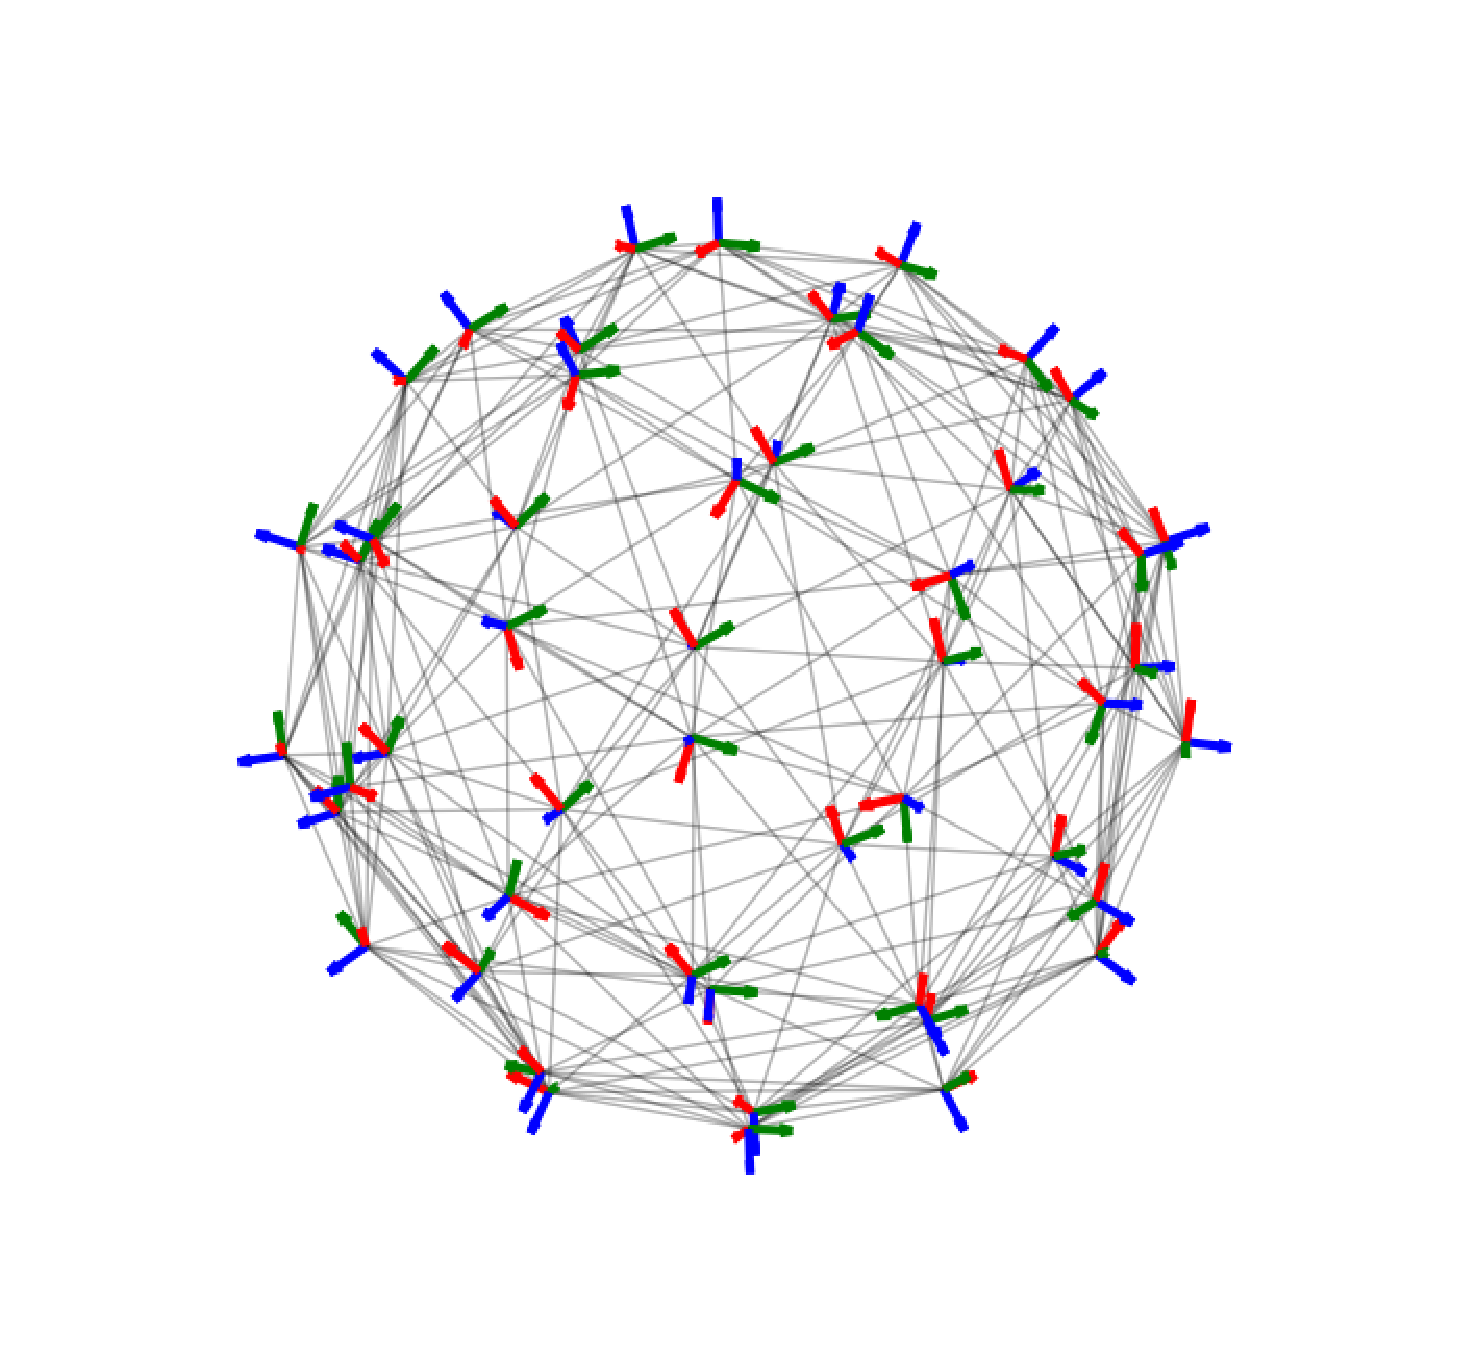
\includegraphics[width=0.45\linewidth]{fig/gt_graph.eps}%
    }
    \hfill
    \subfloat[DPGO result in an outlier environment (40\% incorrect edges)\label{fig:messy_graph}]{%
        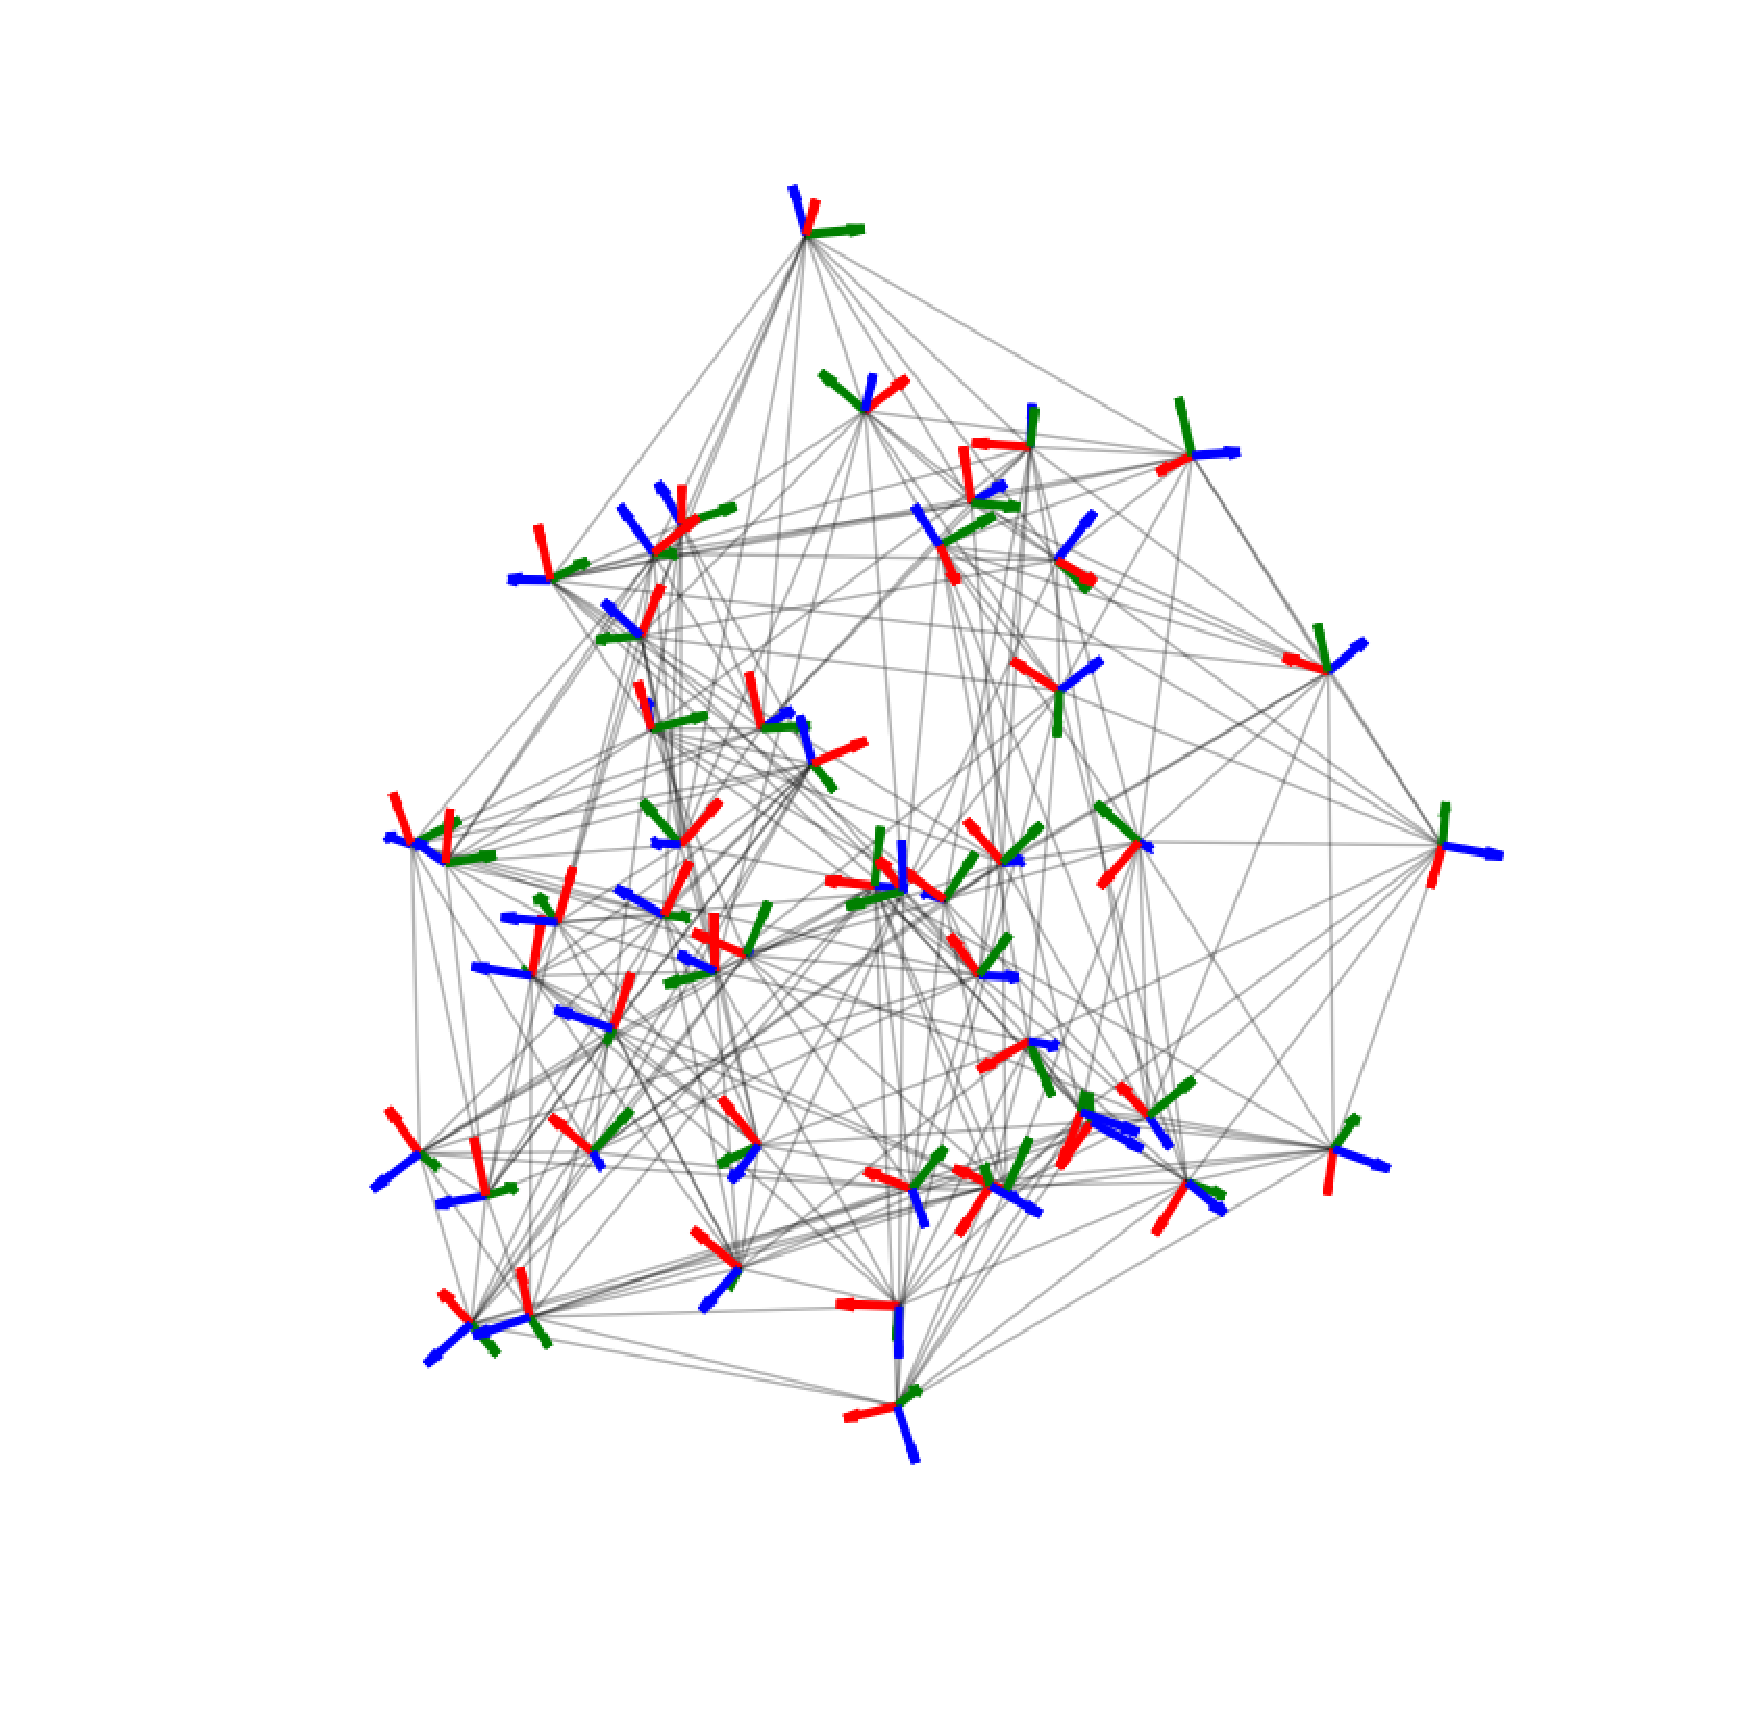
\includegraphics[width=0.45\linewidth]{fig/messy_graph.eps}%
    }
    \caption{Comparison of ground truth and DPGO performance in an outlier-rich environment.}
    \label{fig:gt_messy_comparison}
\end{figure}

In this section, we further evaluate the performance of the proposed method in environments with and without outliers.
We compare our method with the proposed method using Gauss-Newton optimization, and Distributed Certifiably Correct Pose-Graph Optimization (DPGO)~\cite{Tian2021}.

\subsection{Environment without Outliers}
\label{subsec:eval_no_outliers}

Figures~\ref{fig:no_outliers_graphs_1} and \ref{fig:no_outliers_graphs_last} show the pose graphs before and after optimization, respectively.
Figure~\ref{fig:no_outliers_edge_errors} shows the time transition of the edge cost $c_{ij}$, and Figure~\ref{fig:no_outliers_particle_variances} shows the time transition of the particle variance for each agent.
Specifically, Figure~\ref{fig:no_outliers_edge_errors} displays the range (shaded area) between the minimum and maximum costs across all connected edges, along with their mean value.
Figure~\ref{fig:no_outliers_particle_variances} similarly shows the range (shaded area) of particle variances across all agents, and their mean value.

\begin{figure}[H]
    \centering
    \subfloat[Before optimization\label{fig:no_outliers_graphs_1}]{%
        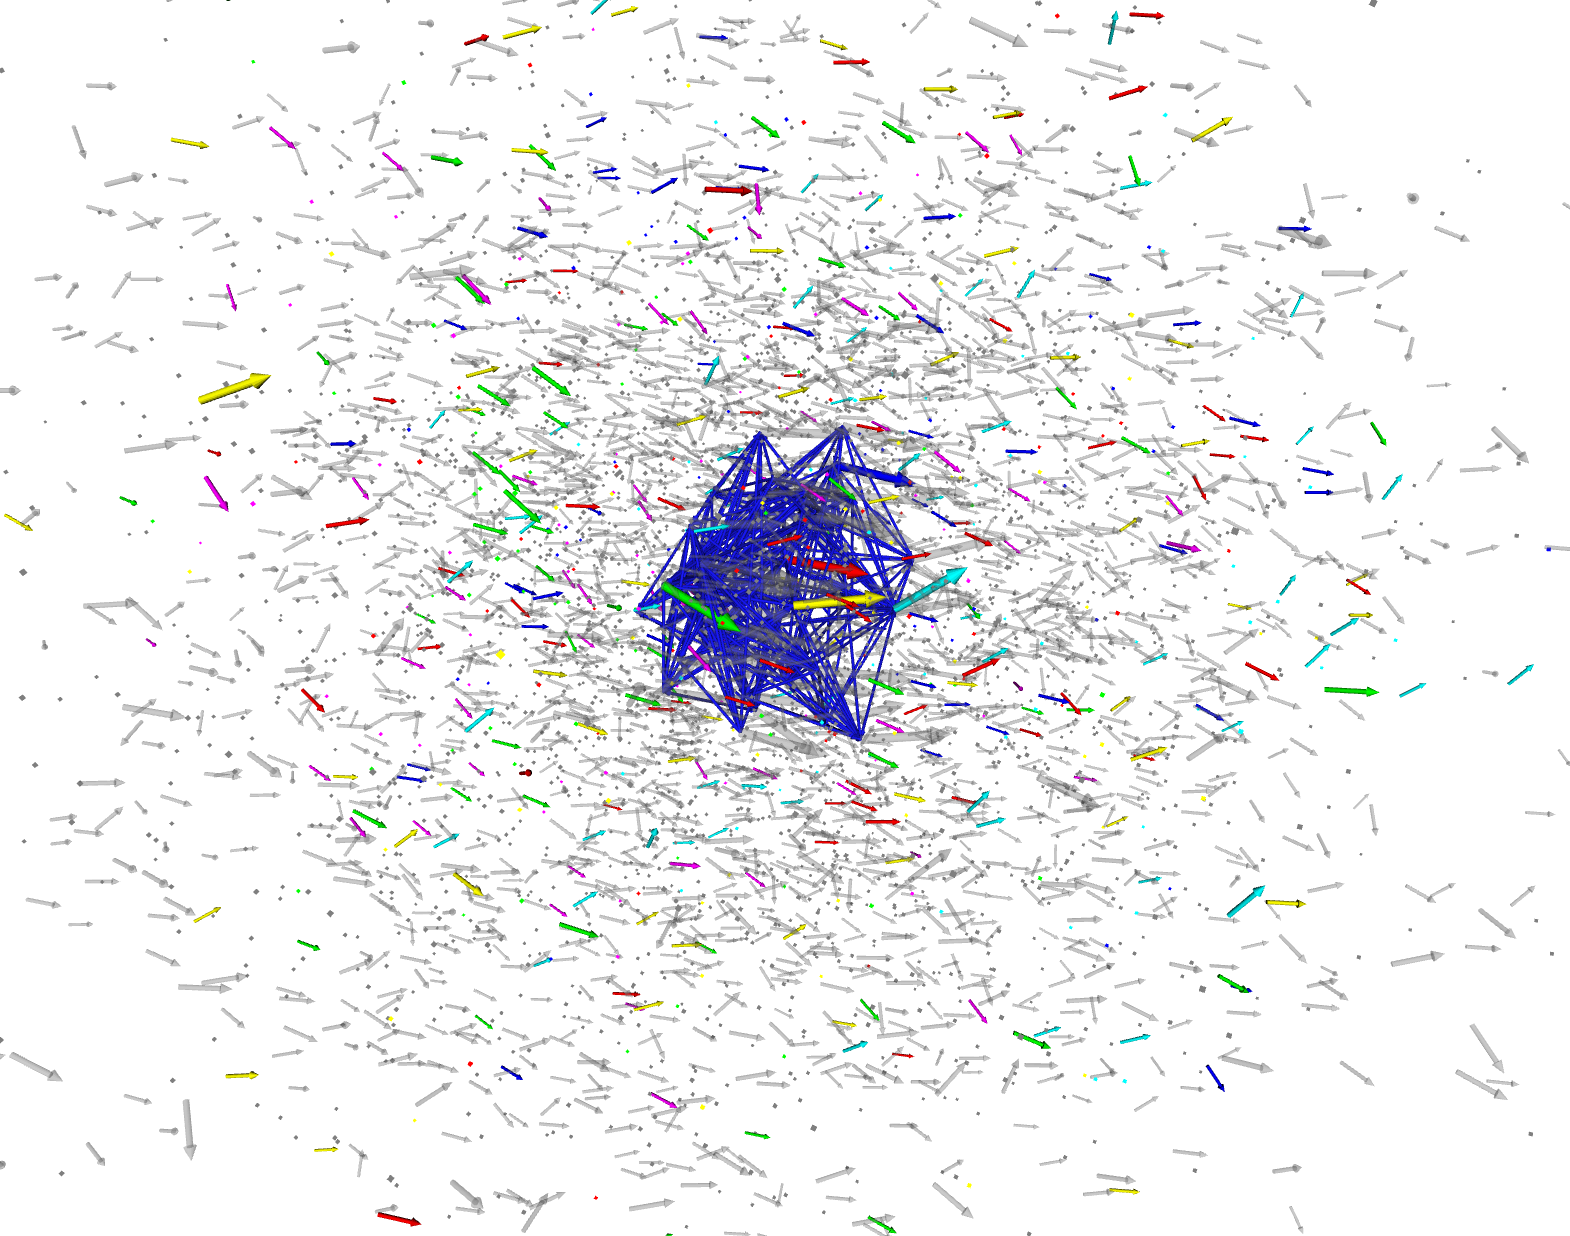
\includegraphics[width=0.45\linewidth]{fig/graph_temp_step_1.eps}%
    }
    \hfill
    \subfloat[After optimization\label{fig:no_outliers_graphs_last}]{%
        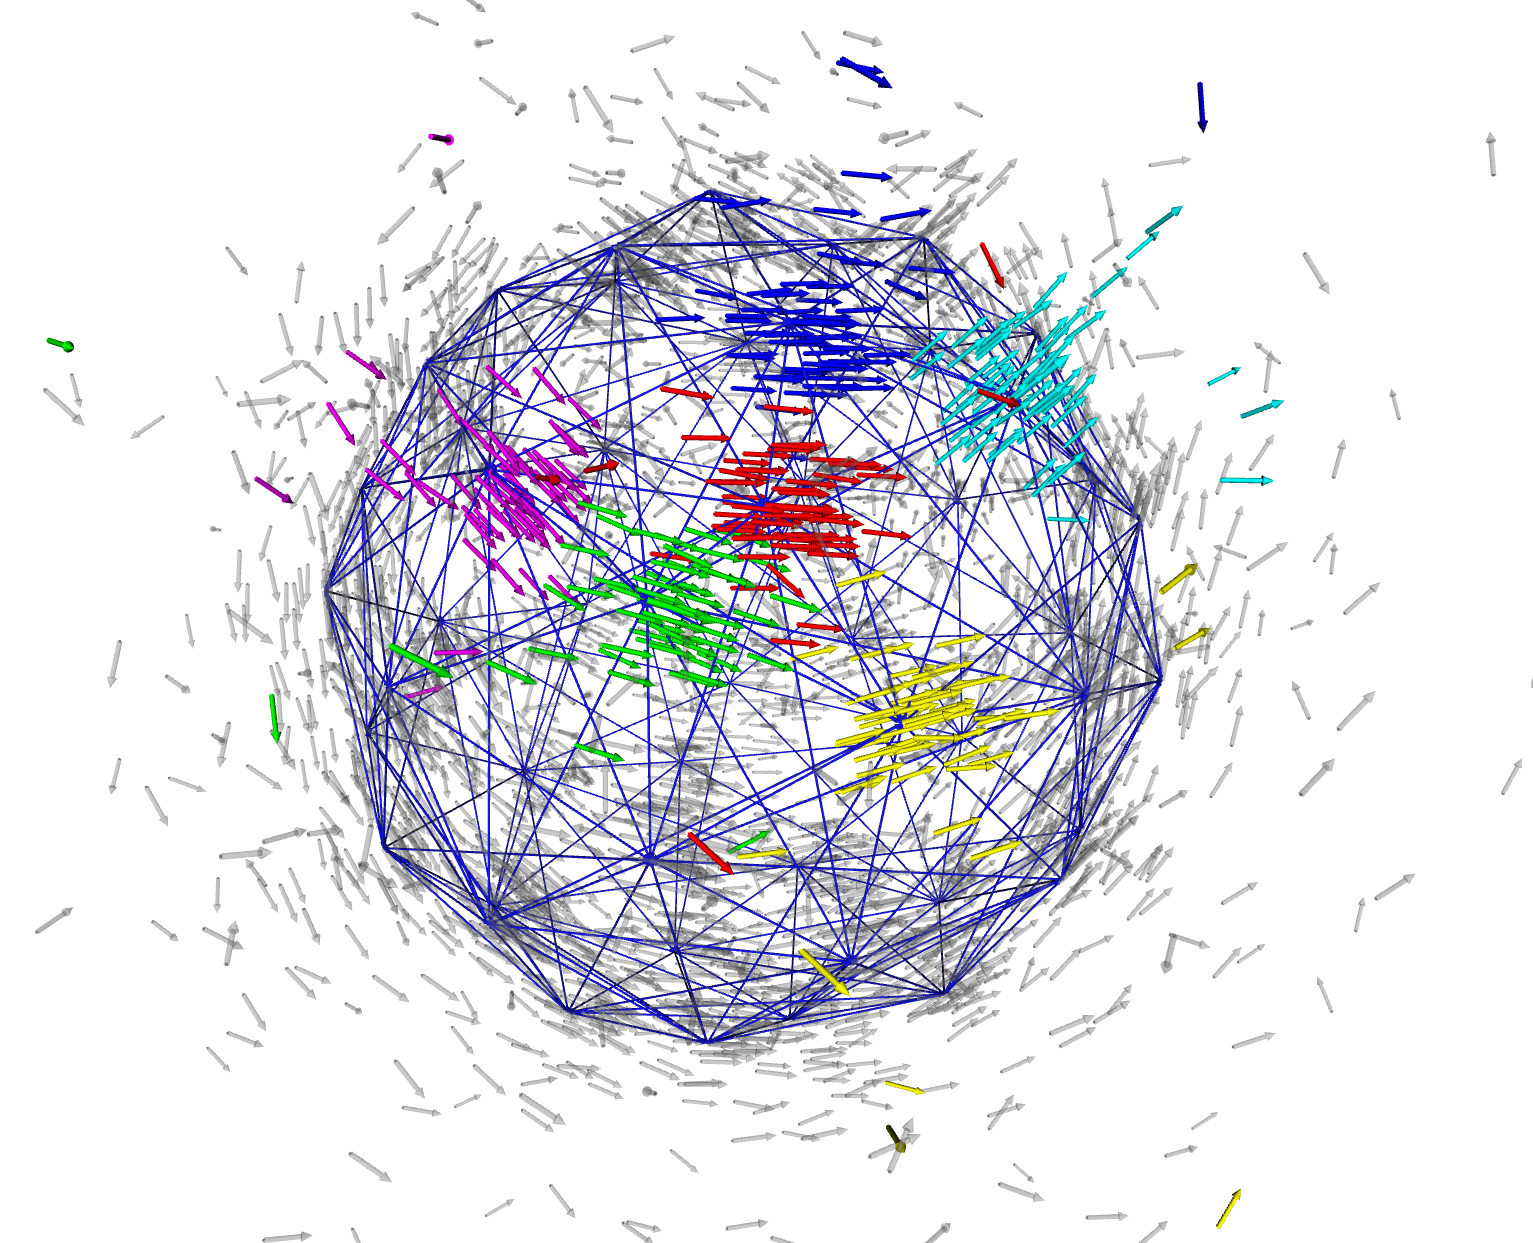
\includegraphics[width=0.45\linewidth]{fig/graph_temp_step_last.eps}%
    }
    \\
    \subfloat[Edge errors $c_{ij}$\label{fig:no_outliers_edge_errors}]{%
        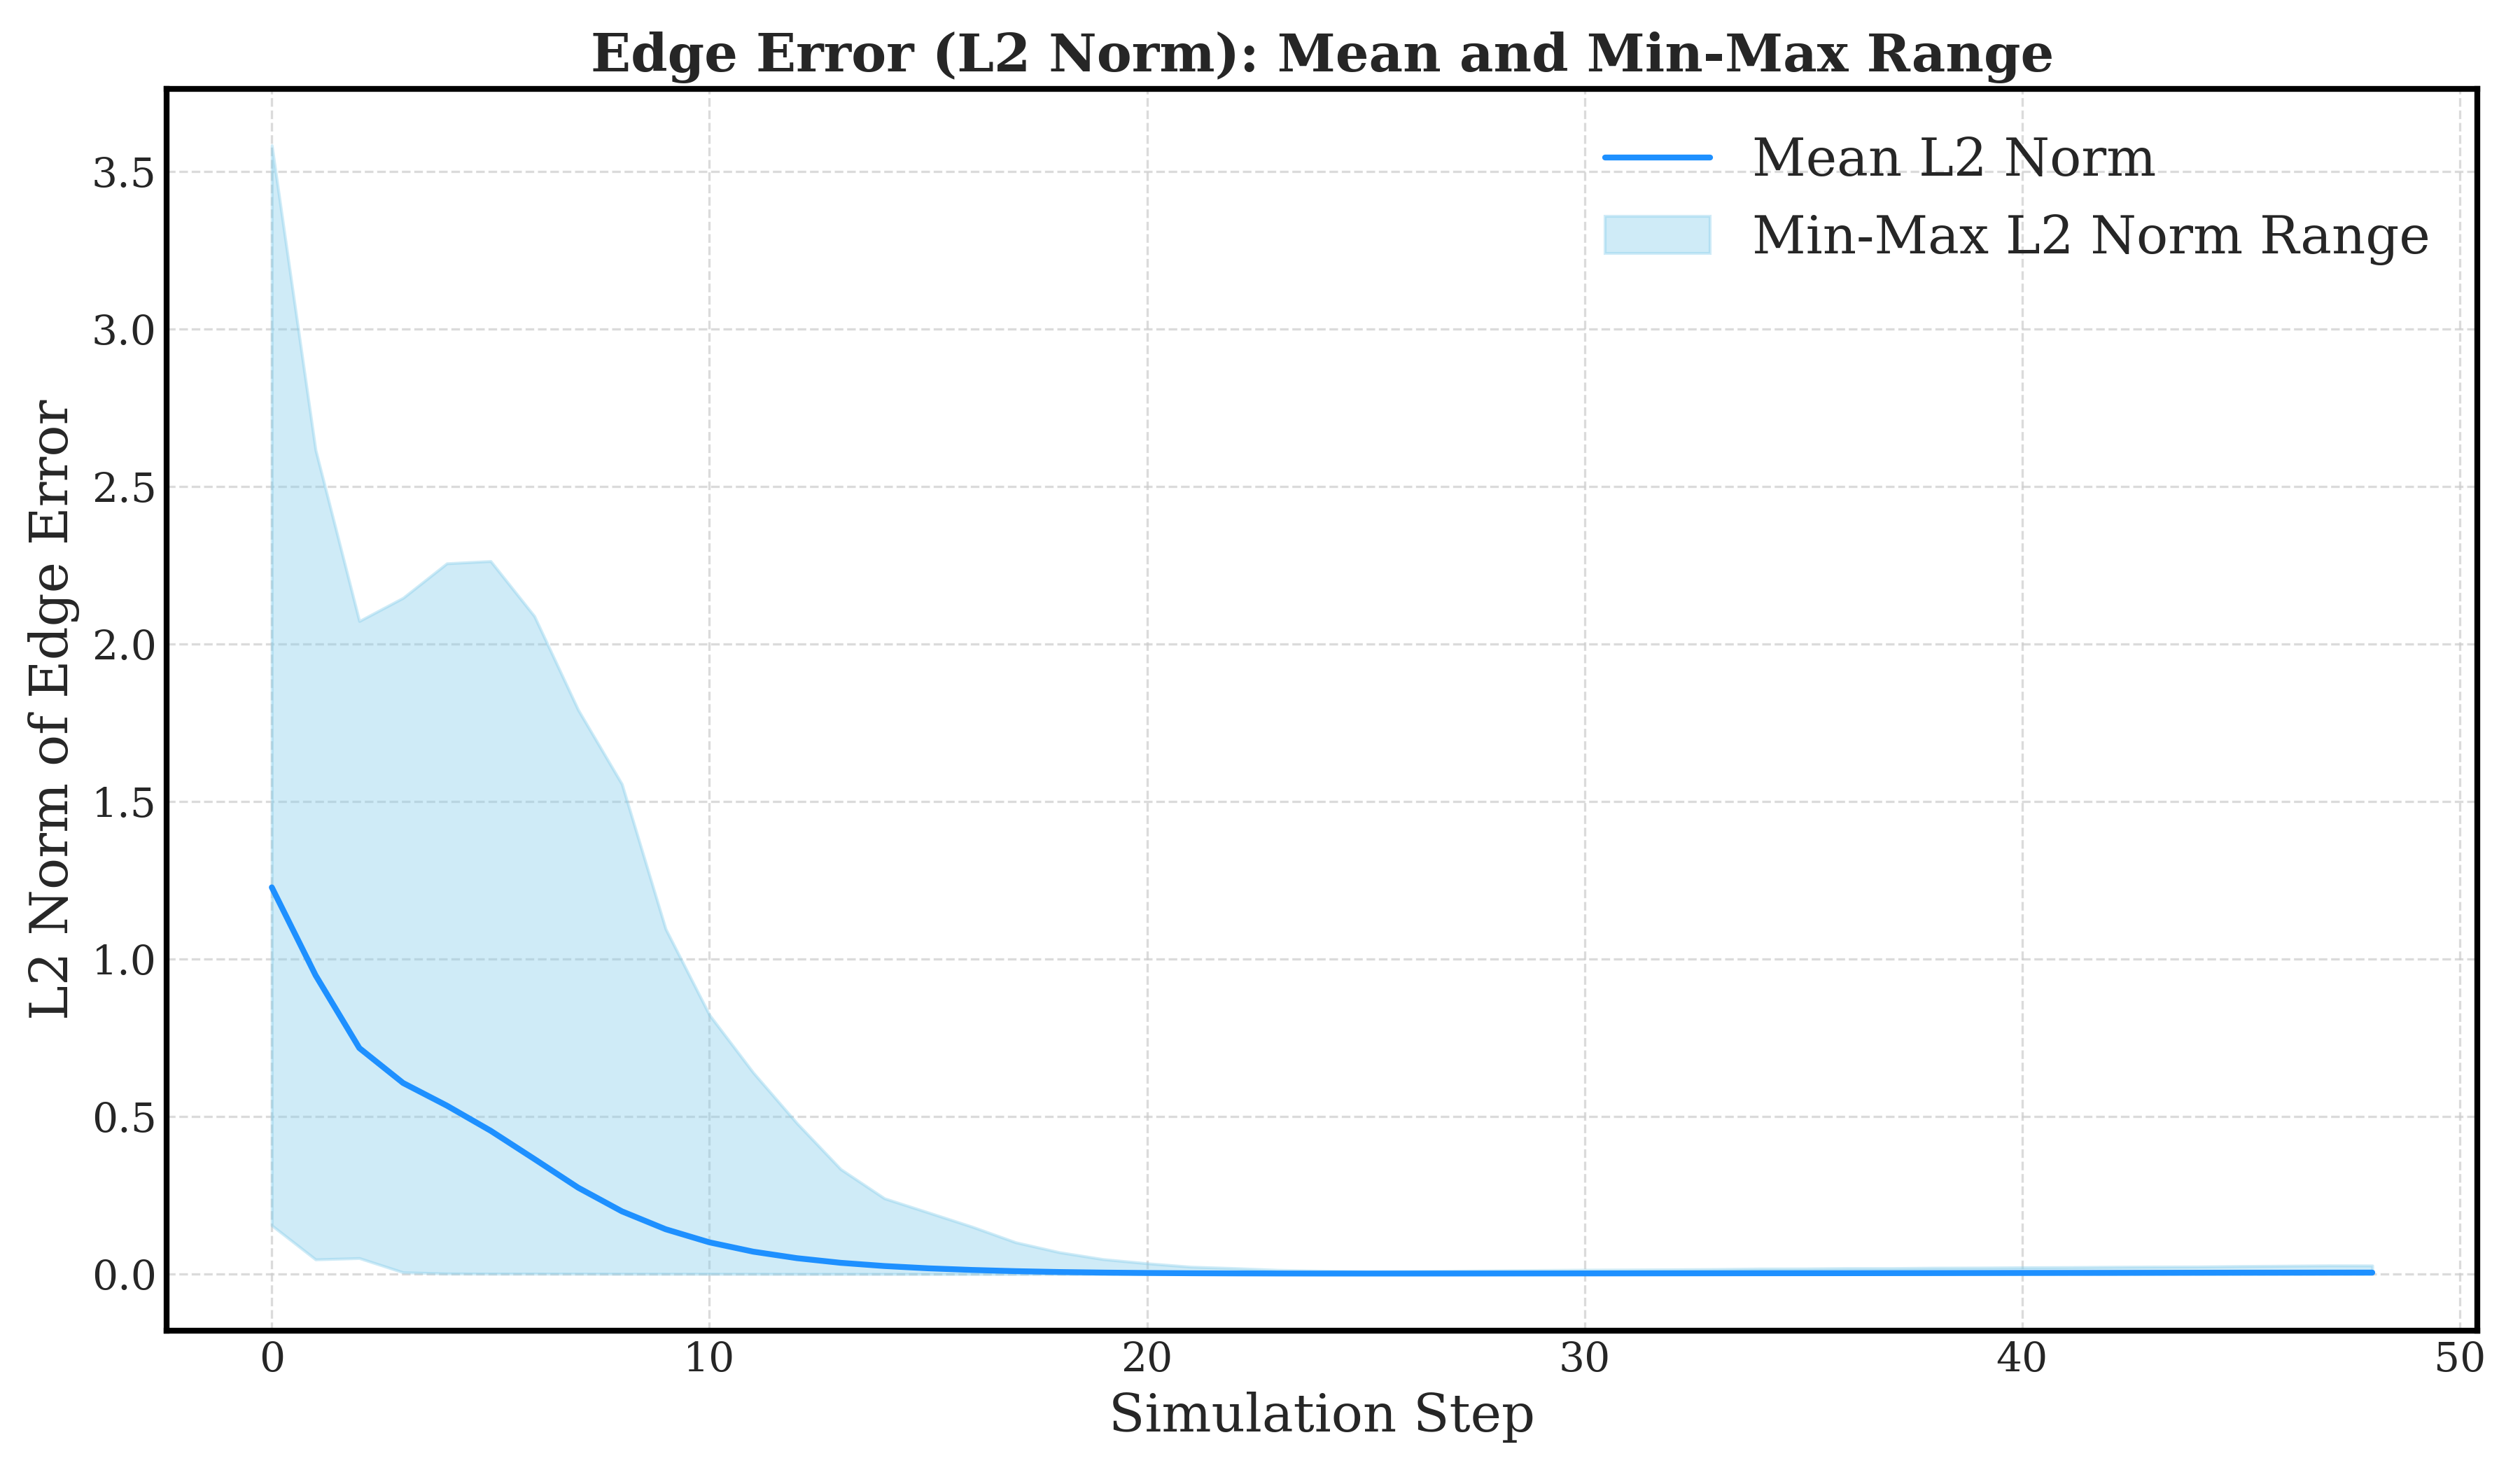
\includegraphics[width=0.45\linewidth]{fig/edge_errors_temp.eps}%
    }
    \hfill
    \subfloat[Particle variances\label{fig:no_outliers_particle_variances}]{%
        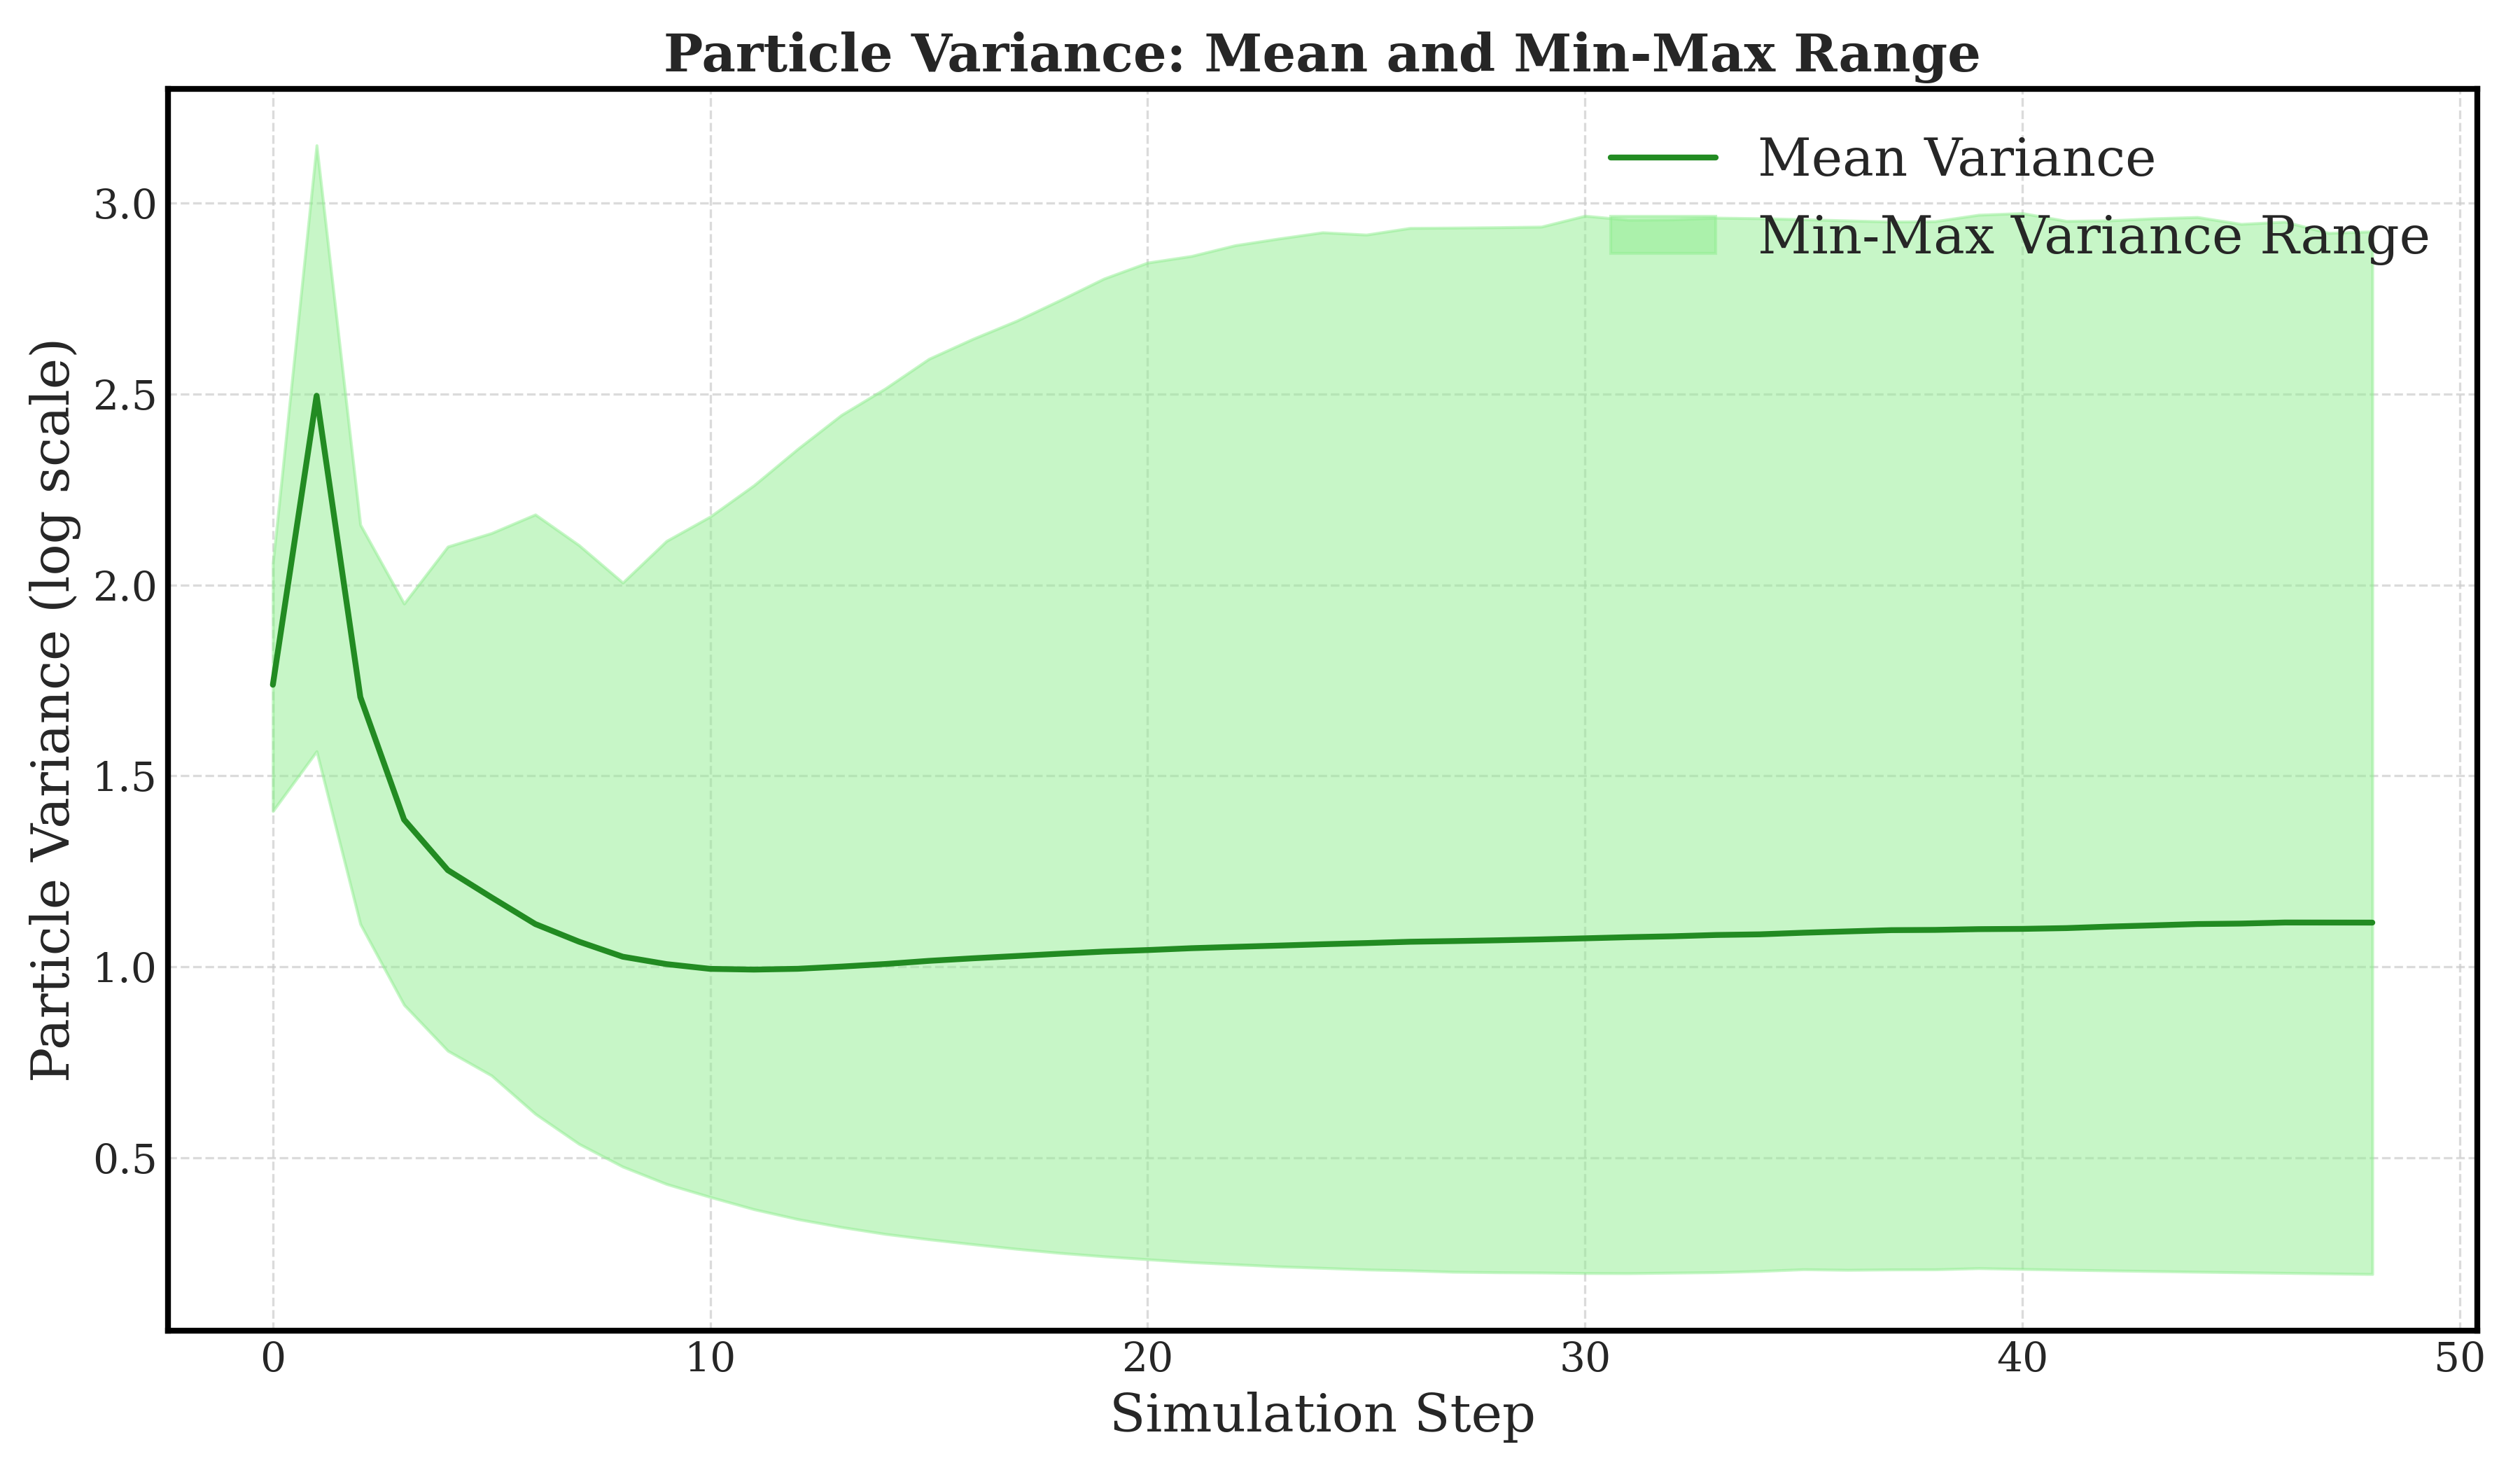
\includegraphics[width=0.45\linewidth]{fig/particle_variances_temp.eps}%
    }
    \caption{Evaluation in an environment without outliers.}
    \label{fig:eval_no_outliers}
\end{figure}

\subsection{Environment with Outliers}
\label{subsec:eval_with_outliers}

In this subsection, we evaluate the performance in an environment with outliers. In this outlier validation (corresponding to Figure~\ref{fig:eval_with_outliers}), incorrect edges are selected at a rate of 0.3 in each step.
Figures~\ref{fig:with_outliers_graphs_1} and \ref{fig:with_outliers_graphs_last} show the pose graphs before and after optimization in an environment with outliers.
Figure~\ref{fig:with_outliers_edge_errors} shows the time transition of the edge cost $c_{ij}$, and Figure~\ref{fig:with_outliers_particle_variances} shows the time transition of the particle variance for each agent.
Specifically, Figure~\ref{fig:with_outliers_edge_errors} displays the range (shaded area) between the minimum and maximum costs across all connected edges, along with their mean value. It shows that although errors occur, they do not diverge and maintain a certain level.
Figure~\ref{fig:with_outliers_particle_variances} similarly shows the range (shaded area) of particle variances across all agents, and their mean value, indicating that outliers cause an increase in particle variance.

\begin{figure}[H]
    \centering
    \subfloat[Before optimization\label{fig:with_outliers_graphs_1}]{%
        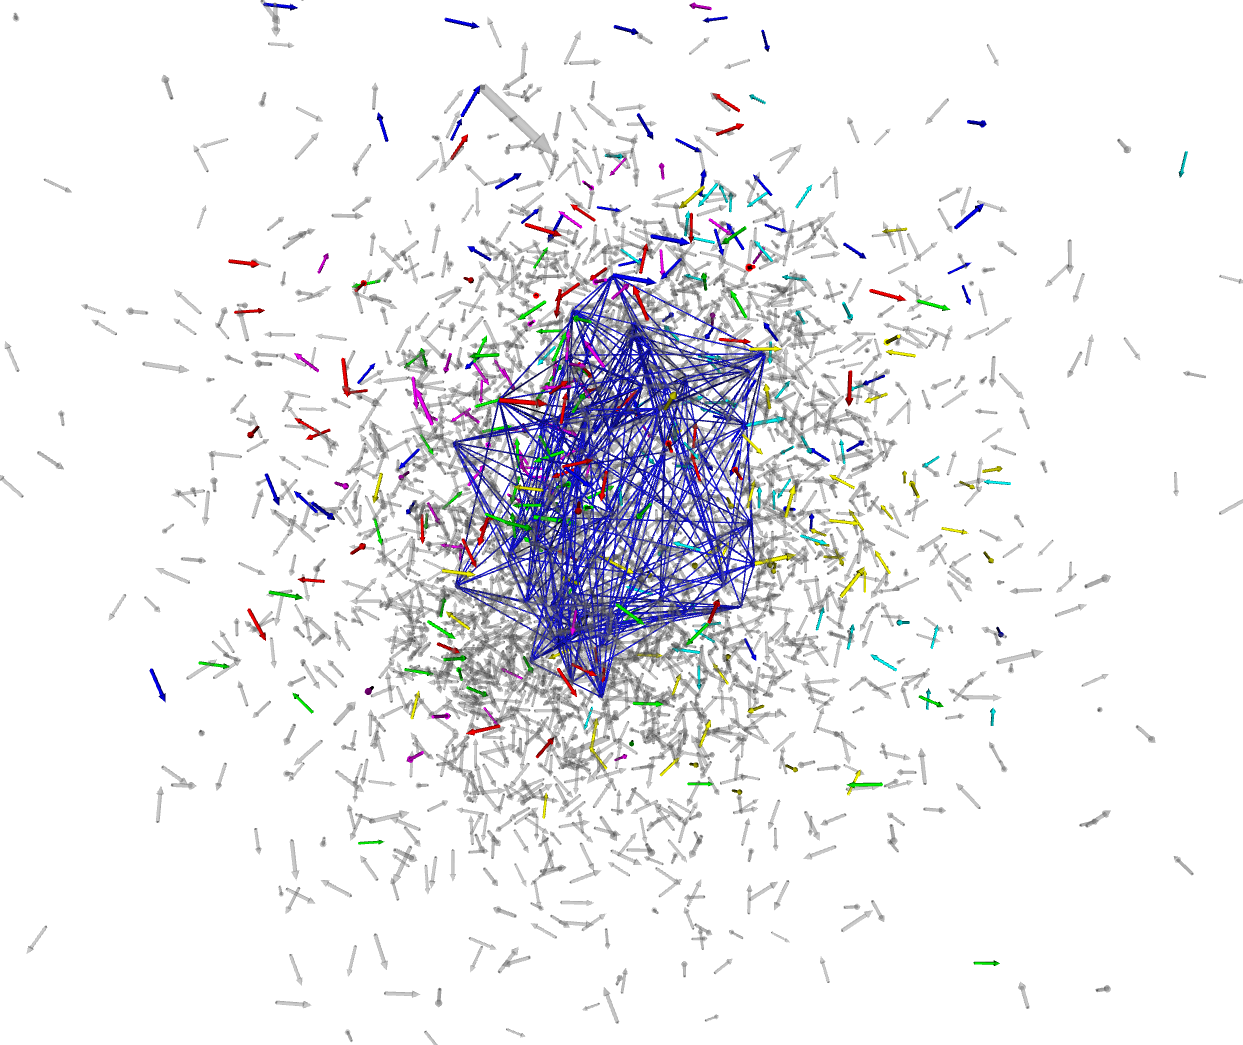
\includegraphics[width=0.45\linewidth]{fig/graph_temp2_step_1.eps}%
    }
    \hfill
    \subfloat[After optimization\label{fig:with_outliers_graphs_last}]{%
        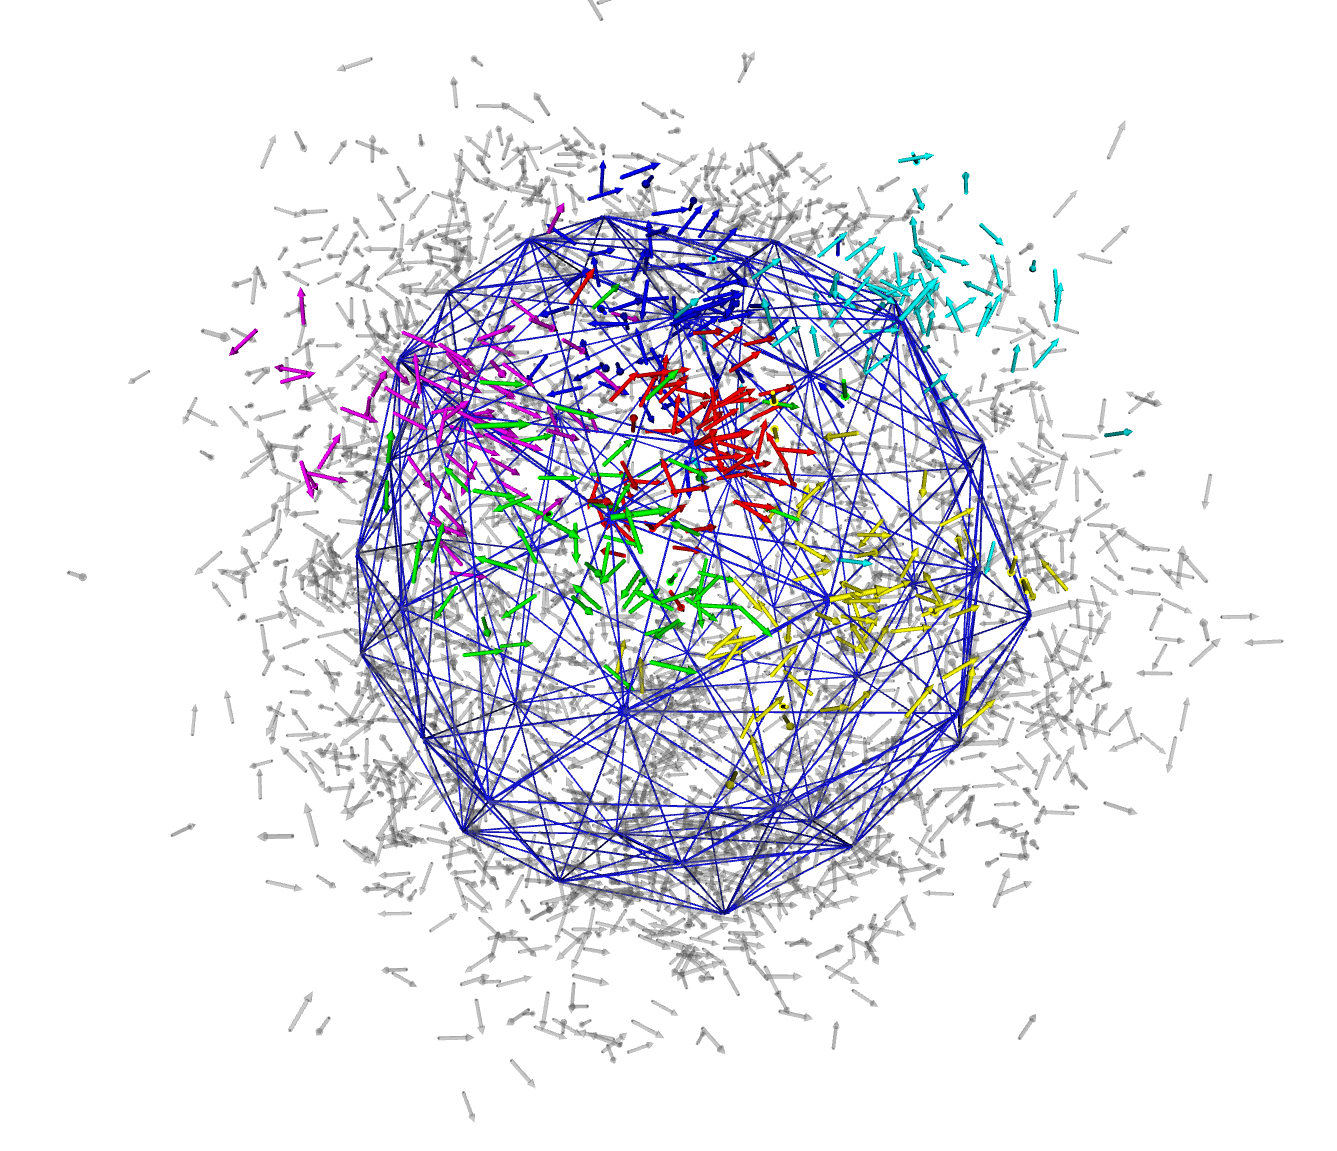
\includegraphics[width=0.45\linewidth]{fig/graph_temp2_step_last.eps}%
    }
    \\
    \subfloat[Edge errors $c_{ij}$\label{fig:with_outliers_edge_errors}]{%
        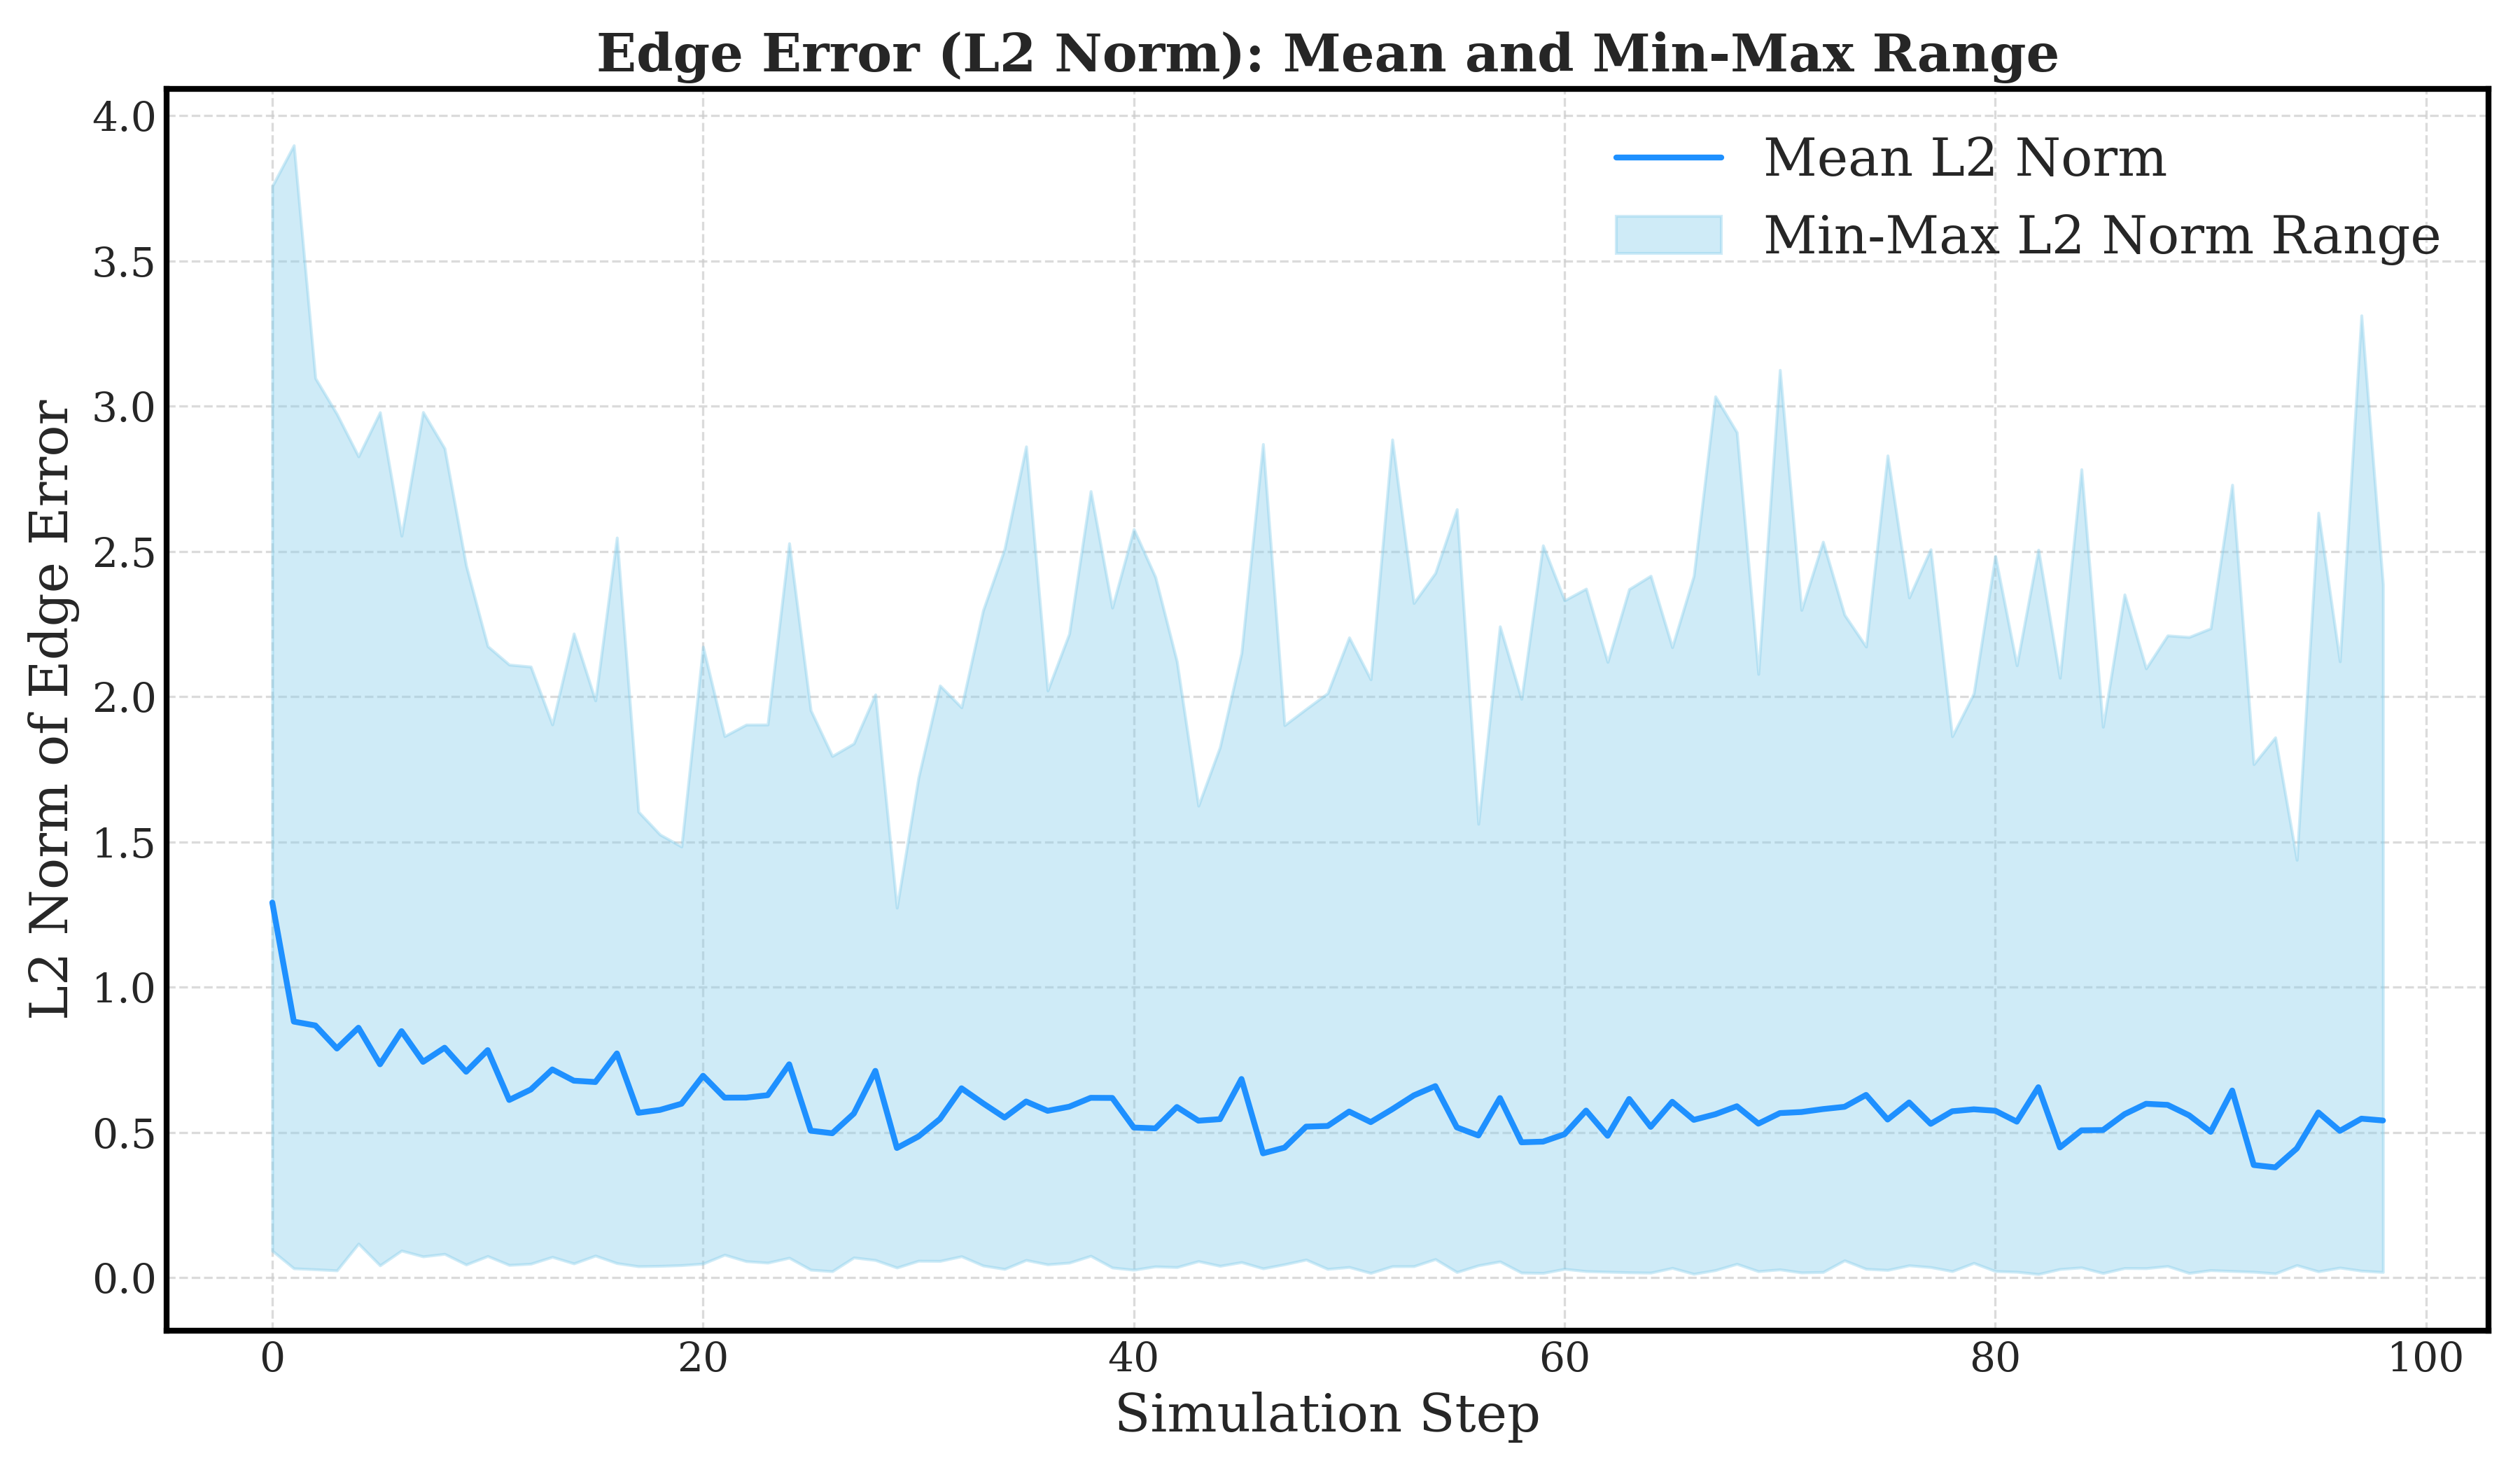
\includegraphics[width=0.45\linewidth]{fig/edge_errors_temp2.eps}%
    }
    \hfill
    \subfloat[Particle variances\label{fig:with_outliers_particle_variances}]{%
        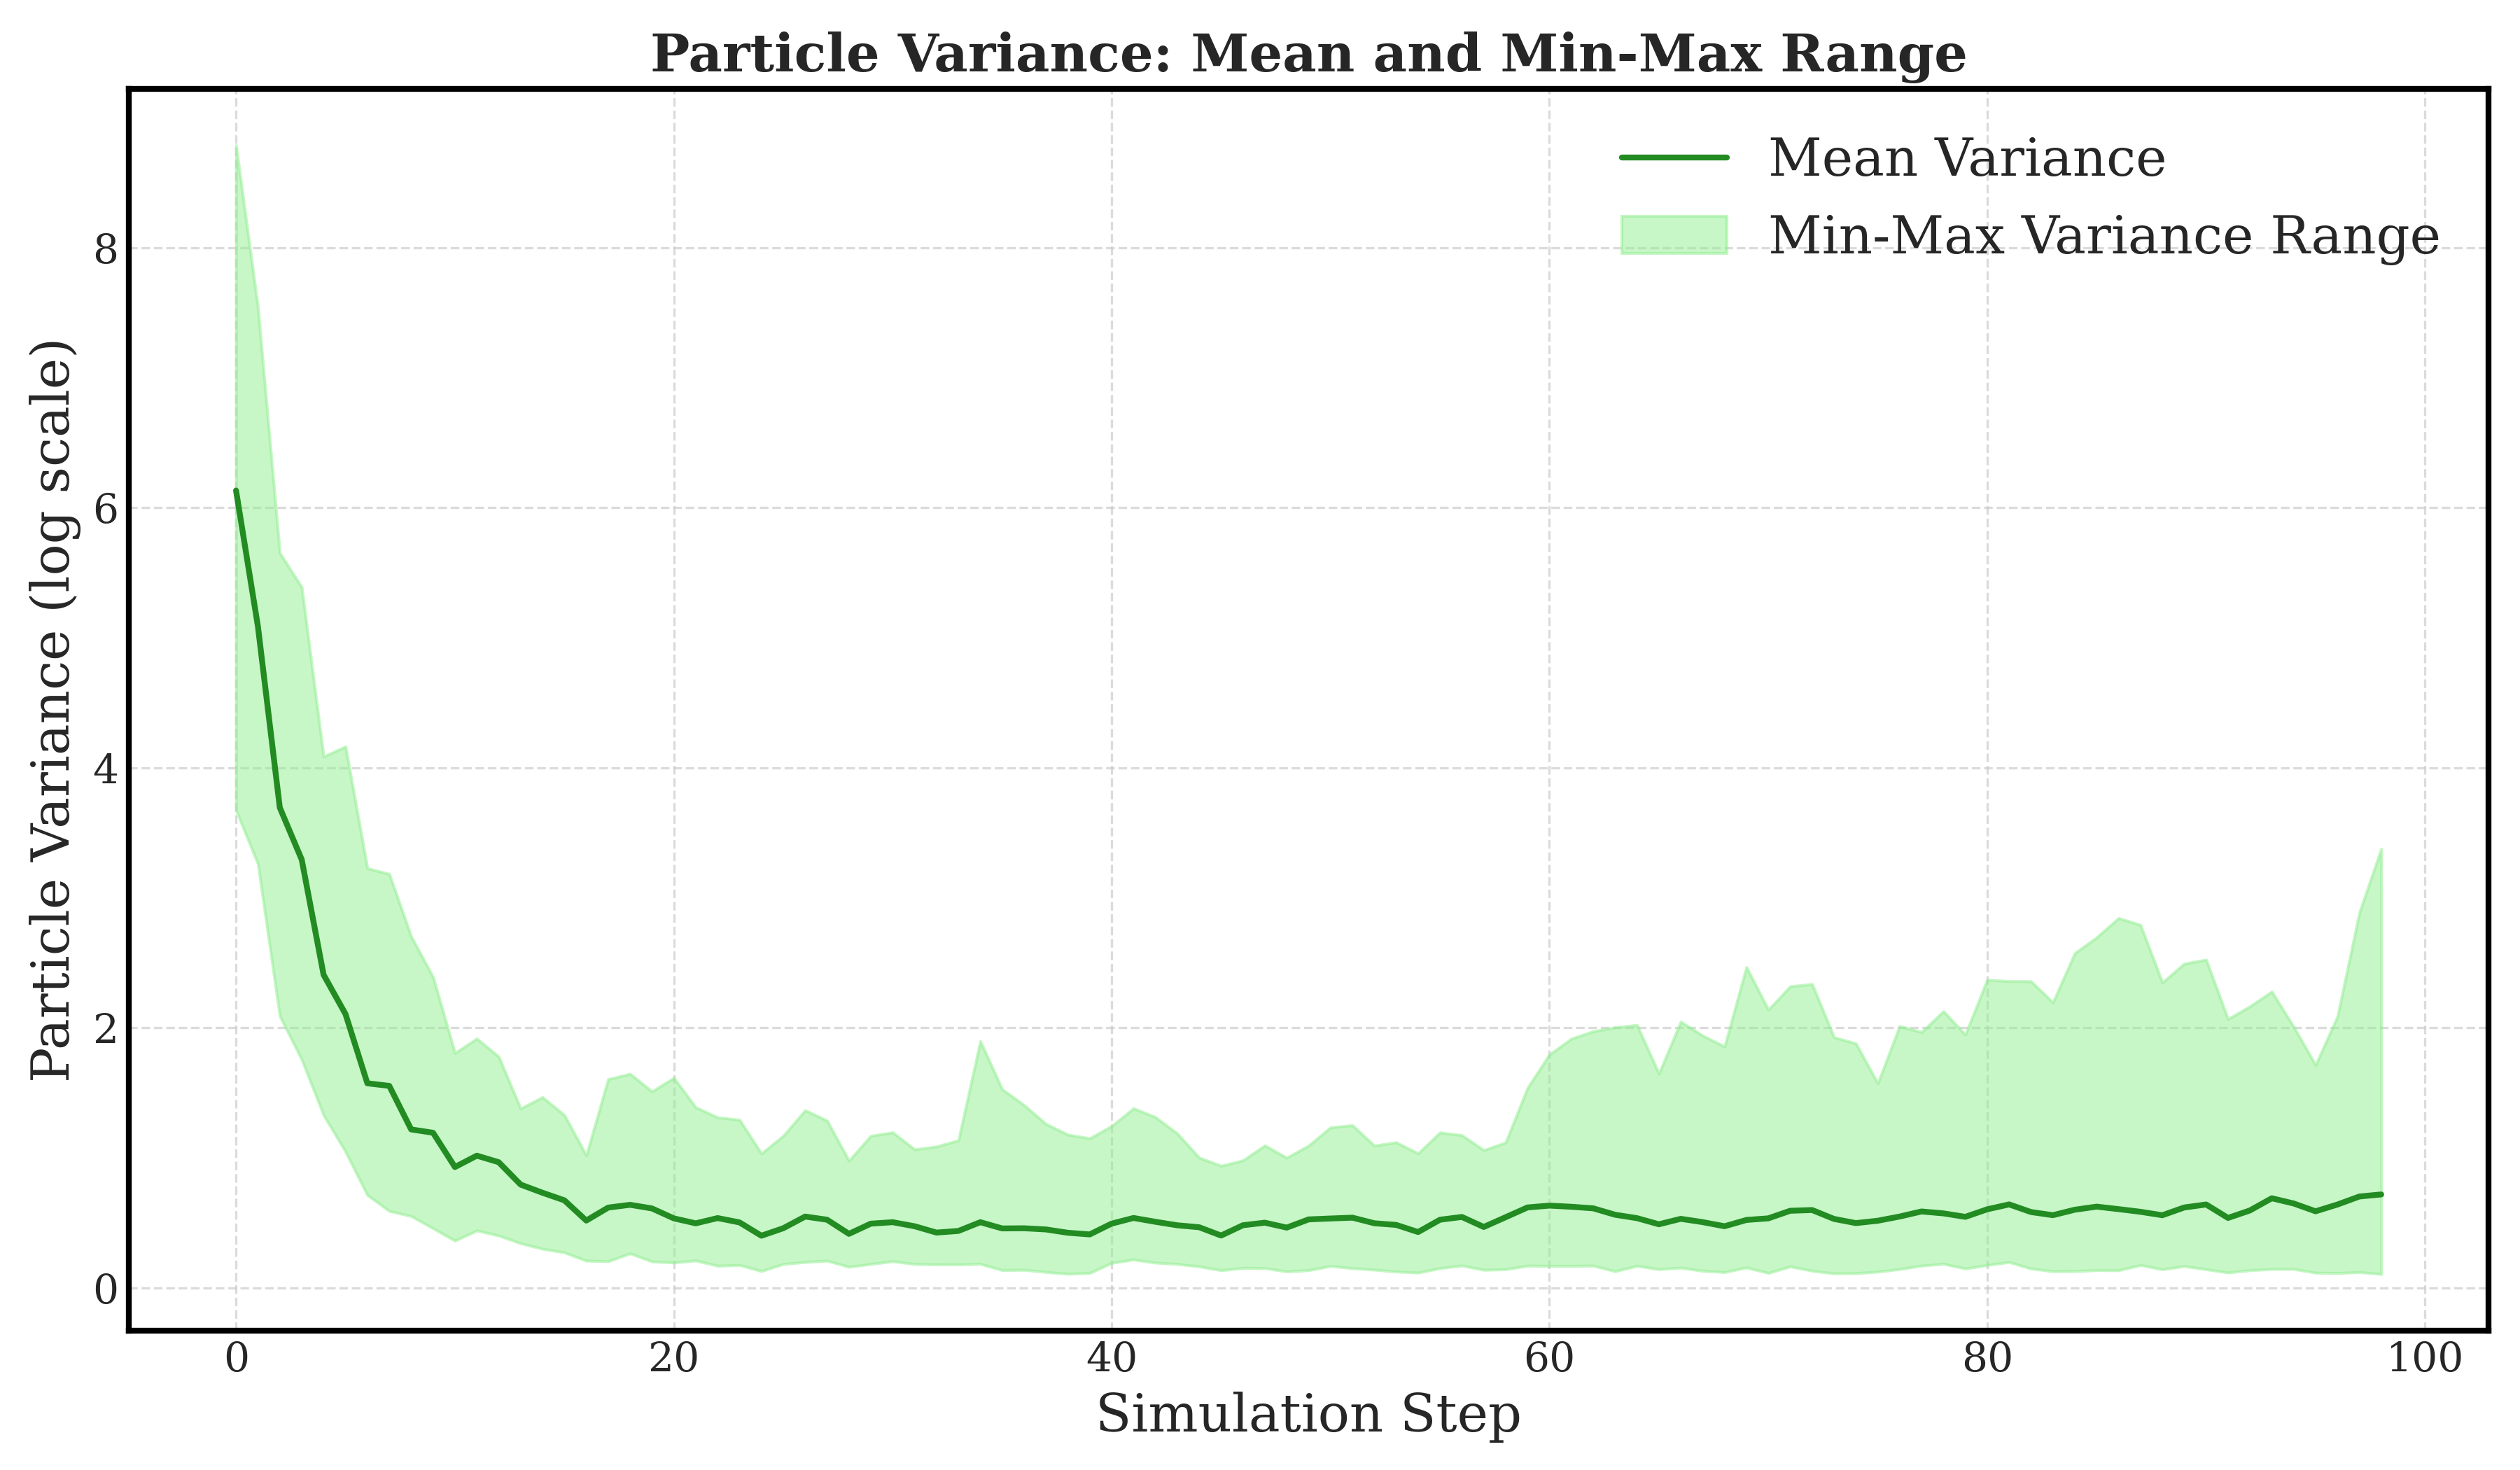
\includegraphics[width=0.45\linewidth]{fig/particle_variances_temp2.eps}%
    }
    \caption{Evaluation in an environment with outliers.}
    \label{fig:eval_with_outliers}
\end{figure}

% \subsection{Benchmark Results}
% \label{subsec:benchmark_results}

In the benchmark comparisons, for DPGO, an optimization problem with incorrectly selected edges based on each outlier ratio is solved. For the proposed method (ASP-PGF), edges are randomly misselected at each of the 50 steps based on the outlier ratio. As demonstrated in our experiments, the algorithm consistently converges to a KKT point (as proven in Theorem 4.1) within 50 iterations in our 20-agent, 1000-particle scenario, confirming the theoretical guarantees.

Table~\ref{tab:benchmark_results} summarizes the performance metrics for each method.
As the outlier ratio increases, the filtering-based proposed method (ASP-PGF) surpasses the accuracy of optimization-based methods like DPGO.

\begin{table}[H]
  \centering
  \caption{Benchmark Results (Single Metric)}
  \label{tab:benchmark_results}
  \begin{tabular}{@{}lccc@{}}
    \toprule
    Environment & DPGO~\cite{Tian2021} & ASP-PGF(GN) \\
    \midrule
    Without Outliers & \textbf{1.10}\times 10^{-11} & 0.026 \\
    Outlier Ratio 0.2 & \textbf{0.216} & 0.591 \\
    Outlier Ratio 0.4 & 0.902 & \textbf{0.742} \\
    \bottomrule
  \end{tabular}
\end{table}

\section{結論及び展望}

本研究では,SE(3)上における協調自己位置推定のための視野共有を保証する分散型CBFを提案した.特に,複数のエージェントが共通の特徴点を観測することで,自己位置推定の精度を向上させるための制御手法を開発した.以下に今後の展望について述べる.

\subsection{確率関数の設計によるアクティブパーセプション}

視野共有を保証するCBFにおいては,特徴点$q_l$がエージェント$i$の視野内にあるかどうかを表す関数$\Psi_{i}^l$が重要な役割を果たす.\Eqref{eq:single_fov_condition}で示したように,この関数は以下のように定義される:
\begin{equation}
\begin{aligned}
\Psi_{i}^l = \left\{ \begin{array}{ll}
0 & \mathrm{if} \quad  \beta_l^{\top}(p_i)R_ie_c-\cos\Psi_{\mathcal{F}} < 0\\
1 & \mathrm{if}  \quad  \beta_l^{\top}(p_i)R_ie_c-\cos\Psi_{\mathcal{F}} \geq 0
\end{array} \right.
\end{aligned}
\label{eq:psi_function}
\end{equation}

しかし,この関数は微分不可能であるため,CBFの設計において問題となる.そこで本研究では,特徴点$q_l \in \mathcal{L}$によってエージェント$i$における推定が成り立っている確率を表す関数$\phi_{i}^l$を導入した:
\begin{equation}
\begin{aligned}
\phi_{i}^l= P(p_i,R_i,q^l)
\end{aligned}
\label{eq:phi_function}
\end{equation}

本研究では,簡単のために以下の確率関数を使用した:
\begin{equation}
\begin{aligned}
P_i^l &= \frac{\beta_l^\top(p_i) R_i e_c -\cos\Psi_{\mathcal{F}} }{1-\cos\Psi_{\mathcal{F}}}
\end{aligned}
\label{eq:p_function}
\end{equation}
ここで,$\beta_l$はエージェント$i$から特徴点$q_l$への単位方向ベクトル,$R_i$はエージェント$i$の姿勢行列,$e_c$はカメラの光軸方向を表す単位ベクトル,$\Psi_{\mathcal{F}}$はカメラの視野角の半分である.この確率関数は,特徴点がカメラの光軸に近いほど高い値を取り,視野角の境界では0になるという性質を持つ.

\subsection{自己位置推定における確率関数の理論的裏付け}

$P^l_i$が$(p_i, R_i)\in \mathrm{SE(3)}$について微分可能であれば,任意の確率関数を設計可能である.本研究では,自己位置推定における理論的な裏付けに基づいた確率関数の設計について検討した.

各エージェント$i \in \mathcal{A}$に対して,観測モデルは以下のように表される:
\begin{equation}
\begin{aligned}
\tilde{p}_i = \pi_i(q_l) + w_i
\end{aligned}
\label{eq:observation_model}
\end{equation}
ここで,$\pi_i(q_l)$はエージェント$i$における$q_l$の非線形な投影関数であり,$w_i$は白色ノイズである.通常,$w_i$は独立同分布の正規分布$w_i \sim \mathcal{N}(0, \sigma_i^2 I)$と仮定される.

最尤推定量$\hat{q}_l$は,以下の最適化問題の解として求められる:
\begin{equation}
\begin{aligned}
\hat{q}_l = \operatorname*{arg\,min}_{q_l} \sum_i \| \tilde{p}_i - \pi_i(q_l) \|^2_{\Sigma_i^{-1}}
\end{aligned}
\label{eq:mle}
\end{equation}
ここで,$\Sigma_i$は$w_i$の共分散行列である.

投影関数$\pi_i(q_l)$は一般に非線形であるため,解析的に誤差伝搬や不確かさを評価するには,$q_l$の推定値の周りで一階テイラー展開を用いる.任意の推定点$q_0^l$周りで:
\begin{equation}
\begin{aligned}
\pi_i(q_l) \approx \pi_i(q_0^l) + J_i (q_l - q_0^l)
\end{aligned}
\label{eq:taylor_expansion}
\end{equation}
と近似する.ここで,$J_i = \frac{\partial \pi_i}{\partial q_l} \Big|_{q_l=q_0^l}$はエージェント$i$における投影関数のヤコビアンである.

最尤推定問題において,推定値の下界としてのCramer-Rao Lower Bound (CRLB)は,フィッシャー情報行列$\mathbf{I}(q_l)$を用いて記述される:
\begin{equation}
\begin{aligned}
\mathbf{I}(q_l) = \sum_i J_i^T \Sigma_i^{-1} J_i
\end{aligned}
\label{eq:fim}
\end{equation}

\begin{dfn}[Cramer--Rao Lower Bound]
確率変数 $\mathbf y\in\mathbb R^{m}$ が母数 $\boldsymbol\theta\in\mathbb R^{p}$ に依存し,
確率密度 $p(\mathbf y;\boldsymbol\theta)$ をもつとする.  
$\hat{\boldsymbol\theta}(\mathbf y)$ が $\boldsymbol\theta$ の不偏推定量
(すなわち $\mathbb E[\hat{\boldsymbol\theta}]=\boldsymbol\theta$)であるとき,
その共分散行列は
\[
    \operatorname{Cov}(\hat{\boldsymbol\theta})
    \;\succeq\;
    \mathbf I(\boldsymbol\theta)^{-1},
    \qquad
    \mathbf I(\boldsymbol\theta)
    :=\mathbb E\!\left[
        \left(\nabla_{\!\boldsymbol\theta}\!\log p(\mathbf y;\boldsymbol\theta)\right)
        \,\left(\nabla_{\!\boldsymbol\theta}\!\log p(\mathbf y;\boldsymbol\theta)\right)^{\!\top}
    \right]
\]
で下から抑えられる.  
ここで $\mathbf I(\boldsymbol\theta)$ は
フィッシャー情報行列と呼ばれる行列である.
この不等式をCramer--Rao Lower Boundと呼ぶ.
\end{dfn}

観測モデル\eqref{eq:observation_model}の下で,パラメータ$q_l$に関する対数尤度関数を
\begin{equation}
\begin{aligned}
\ell(q_l)
&= -\frac{1}{2}\sum_{i=1}^m
(\tilde p_i - \pi_i(q_l))^\top \Sigma_i^{-1}(\tilde p_i - \pi_i(q_l)) + C
\label{eq:loglikelihood_expanded}
\end{aligned}
\end{equation}
と書く。ここで$C$は$q_l$に依存しない定数である。

まず,$\ell(q_l)$の勾配(一次微分)を計算すると
\begin{equation}
\begin{aligned}
\nabla_{q_l}\ell(q_l)
&= \sum_{i=1}^m
\frac{\partial \pi_i}{\partial q_l}^\top
\Sigma_i^{-1}(\tilde p_i - \pi_i(q_l))
= \sum_{i=1}^m J_i^\top \Sigma_i^{-1}(\tilde p_i - \pi_i(q_l)),
\end{aligned}
\label{eq:grad_loglikelihood}
\end{equation}
となる。

次に,二次微分(ヘッセ行列)を取ると
\begin{equation}
\begin{aligned}
\nabla^2_{q_l}\ell(q_l)
&= -\sum_{i=1}^m
J_i^\top \Sigma_i^{-1} J_i
\;+\;\underbrace{\sum_{i=1}^m
(\tilde p_i - \pi_i(q_l))^\top
\Sigma_i^{-1}
\frac{\partial^2 \pi_i}{\partial q_l^2}}_{A(q_l)}.
\end{aligned}
\label{eq:hessian_loglikelihood}
\end{equation}
ガウス雑音の性質より,期待値を取ると残差項$(\tilde p_i - \pi_i)$の平均は零になるため
\begin{equation}
\begin{aligned}
-\mathbb{E}\bigl[\nabla^2_{q_l}\ell(q_l)\bigr]
&= \sum_{i=1}^m J_i^\top \Sigma_i^{-1} J_i.
\end{aligned}
\label{eq:FIM_derivation}
\end{equation}

以上より任意の不偏推定量$\hat{q}_l$の共分散行列は次の下界を満たす:
\begin{equation}
\begin{aligned}
\operatorname{Cov}(\hat{q}_l) \ge \mathbf{I}(q_l)^{-1} = \left( \sum_i J_i^T \Sigma_i^{-1} J_i \right)^{-1}
\end{aligned}
\label{eq:crlb}
\end{equation}

特に,各エージェントのノイズが等方性(すべて$\Sigma_i = \sigma^2 I$とする場合),上式は以下のように簡略化される:
\begin{equation}
\begin{aligned}
\operatorname{Cov}(\hat{q}_l) \ge \sigma^2 \left( \sum_i J_i^T J_i \right)^{-1}
\end{aligned}
\label{eq:crlb_isotropic}
\end{equation}

この式から,エージェント数が増えることにより各々の寄与が積み重なり,結果として推定の不確かさが低下する傾向が明確となる.
各エージェントについて,対象$q_l$の投影に関する解析的なヤコビアンは以下のように記述できる:
\begin{equation}
\begin{aligned}
J_i = \frac{f}{d_i}\,P_{\beta_i}, \quad d_i = \|q_l-p_i\|, \quad P_{\beta_i} = I - \beta_i\,\beta_i^\top
\end{aligned}
\label{eq:jacobian}
\end{equation}
ここで,$f$は焦点距離,$d_i$は対象とエージェント$i$との距離,$\beta_i = \frac{q_l-p_i}{d_i}$はエージェント$i$におけるbearing,$P_{\beta_i}$は$\beta_i$に沿った成分を取り除く射影行列である.

エージェント$i$と$j$からのフィッシャー情報行列は以下のように計算できる:
\begin{equation}
\begin{aligned}
I_i &= J_i^\top J_i = \frac{f^2}{d_i^2}\,P_{\beta_i} \\
I_j &= J_j^\top J_j = \frac{f^2}{d_j^2}\,P_{\beta_j}
\end{aligned}
\label{eq:fim_individual}
\end{equation}

したがって,2台のカメラからの合成情報は以下のようになる:
\begin{equation}
\begin{aligned}
I_{\text{total}} = J_i^\top J_i + J_j^\top J_j = \frac{f^2}{d_i^2}\,P_{\beta_i} + \frac{f^2}{d_j^2}\,P_{\beta_j}
\end{aligned}
\label{eq:fim_total}
\end{equation}

CRLBにより,無偏推定量$\hat{q}_l$の共分散行列は以下の下界を満たす:
\begin{equation}
\begin{aligned}
\operatorname{Cov}(q_l) \ge \sigma^2\,\frac{1}{f^2}\,\left[\frac{P_{\beta_i}}{d_i^2} + \frac{P_{\beta_j}}{d_j^2}\right]^{-1}
\end{aligned}
\label{eq:crlb_two_cameras}
\end{equation}

上記の理論的考察に基づき,新しい確率関数を以下のように設計することができる:
\begin{equation}
\begin{aligned}
P_i^l &= \exp\left(-\frac{\sigma^2}{f^2}\,\mathrm{tr}\left[\frac{P_{\beta_i}}{d_i^2} + \frac{P_{\beta_j}}{d_j^2}\right]^{-1}\right)
\end{aligned}
\label{eq:new_probability_function}
\end{equation}

\Figref{fig:drone_setup}に示すようにエージェントを設置した場合,エージェント$i$と$j$の視野錐台が接する断面における確率関数の値をそれぞれ\Figref{fig:potential_comparison}に示す

\begin{figure}[H]
    \centering
    \begin{subfigure}[b]{0.45\linewidth}
        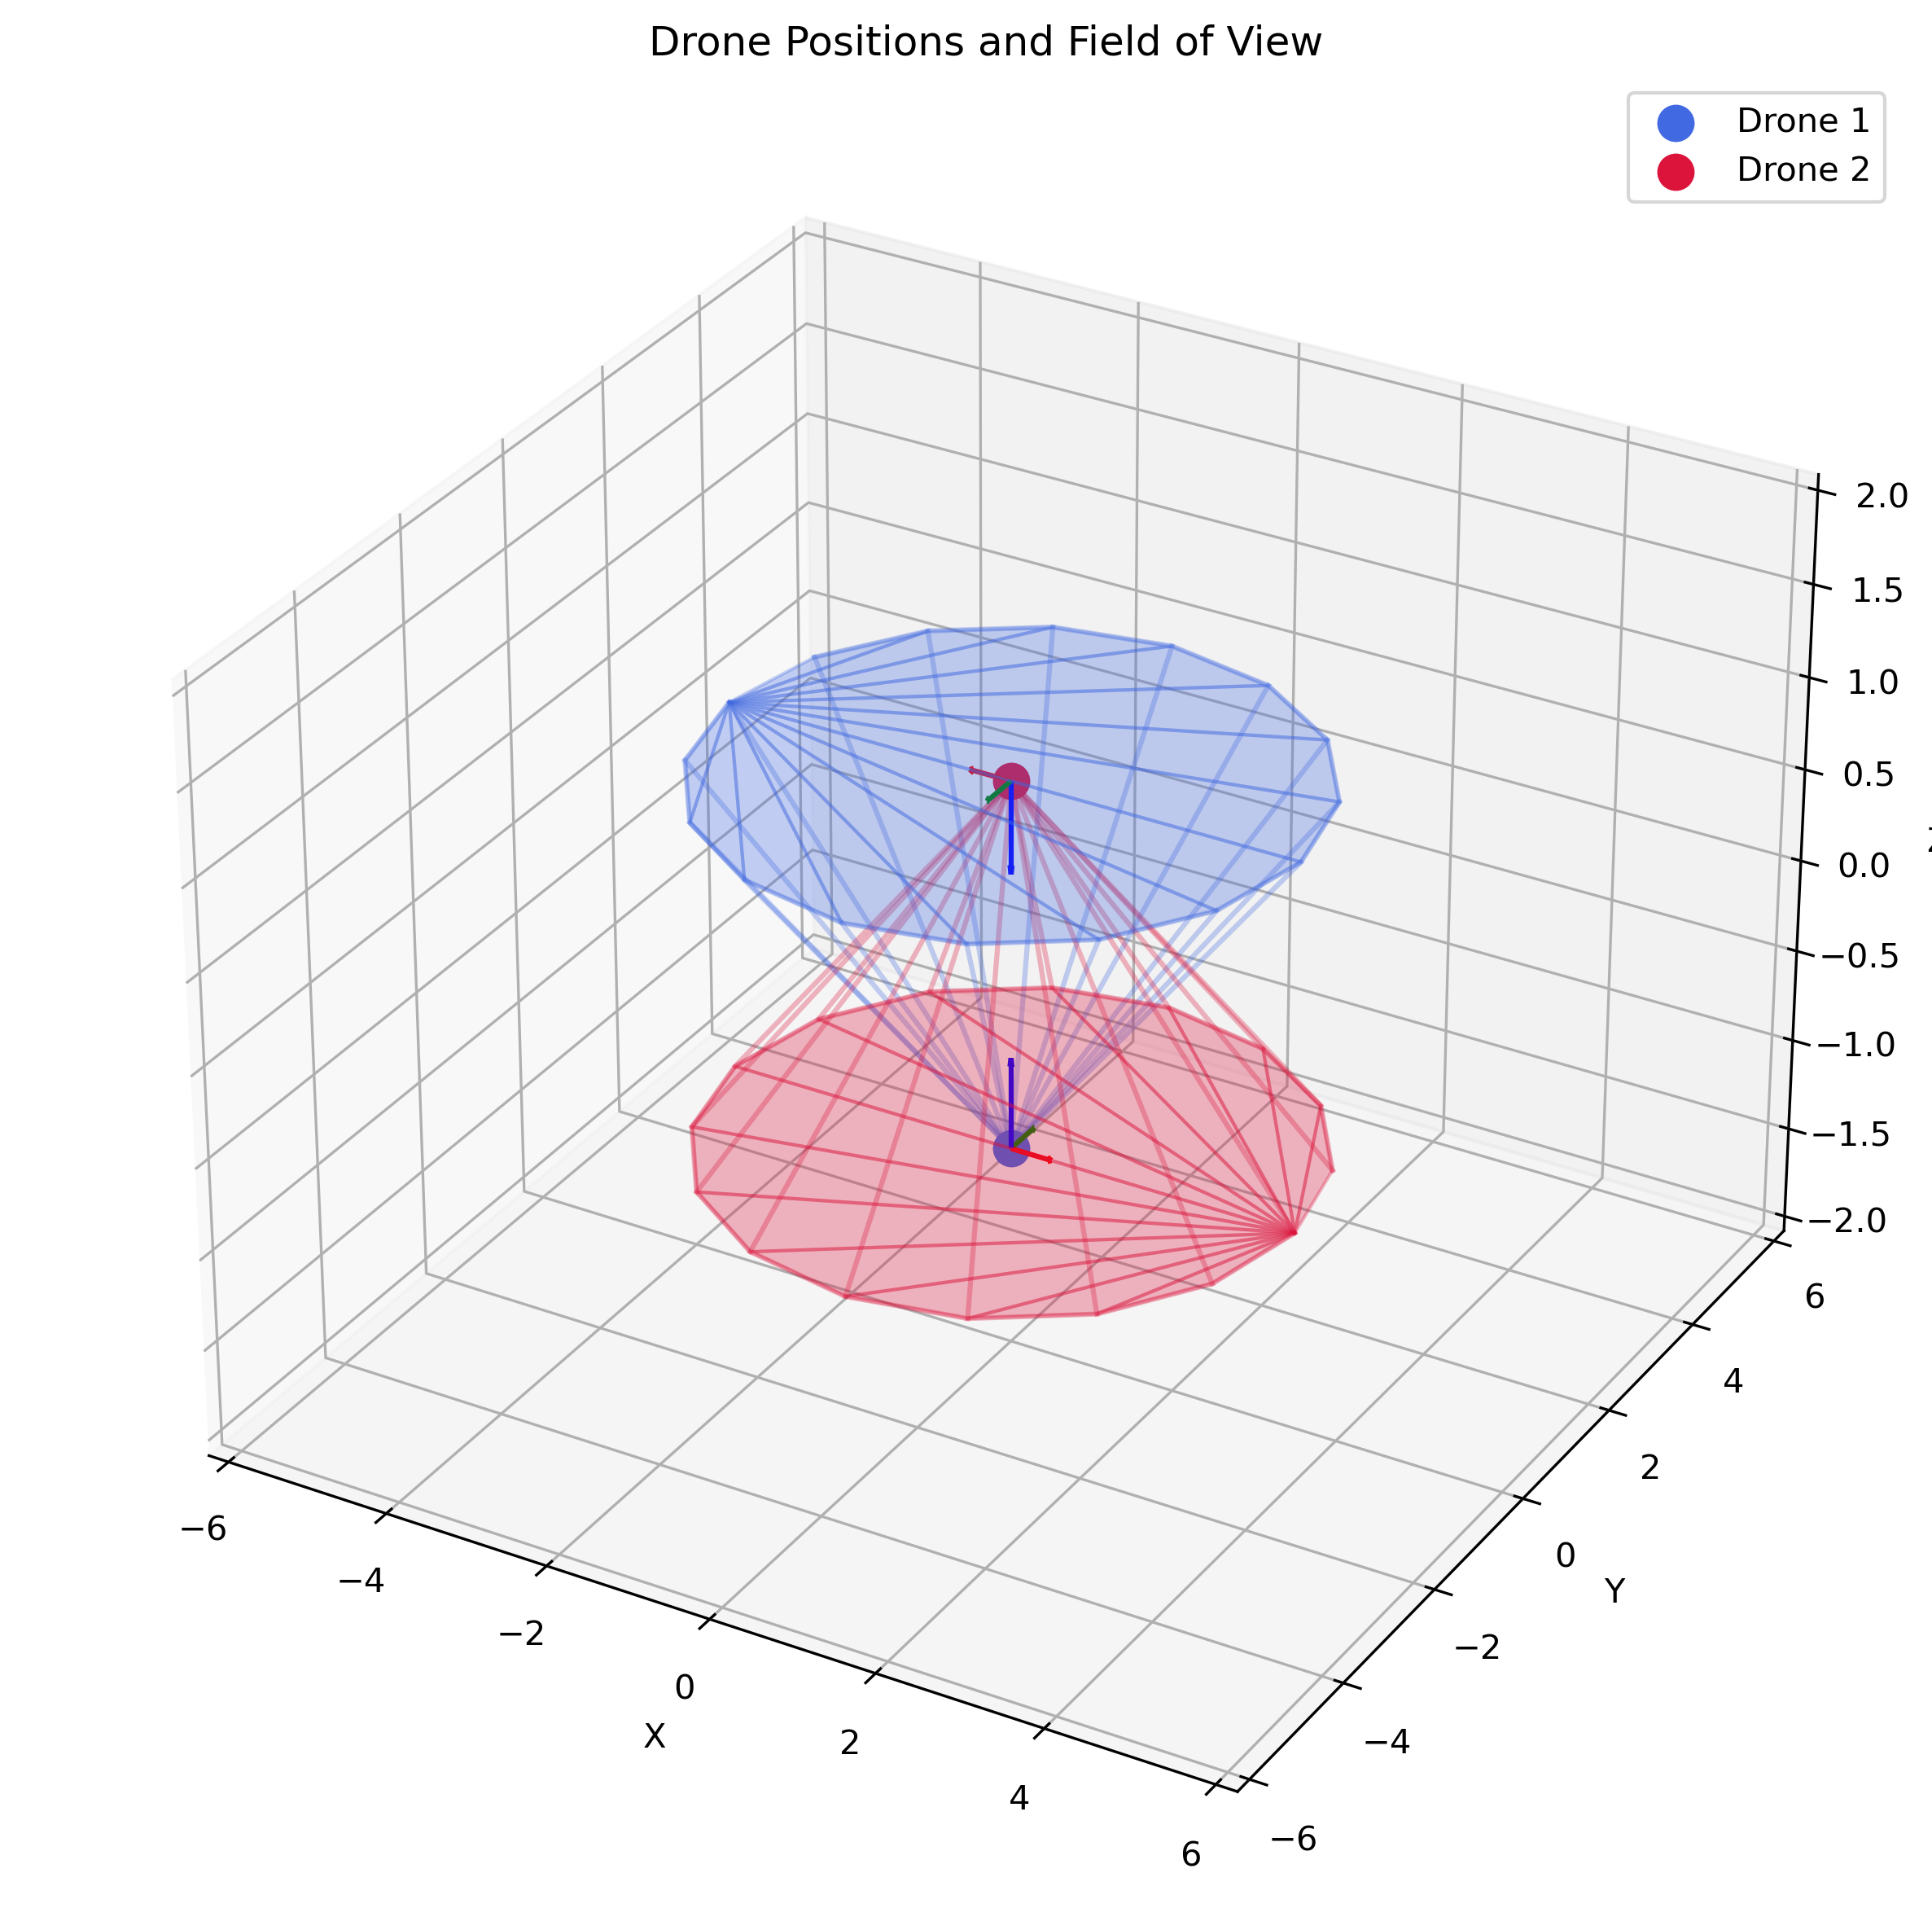
\includegraphics[width=\linewidth]{fig/drone_setup.png}
        \caption{エージェントの設置例}
        \label{fig:drone_setup}
    \end{subfigure}
    \hfill
    \begin{subfigure}[b]{0.45\linewidth}
        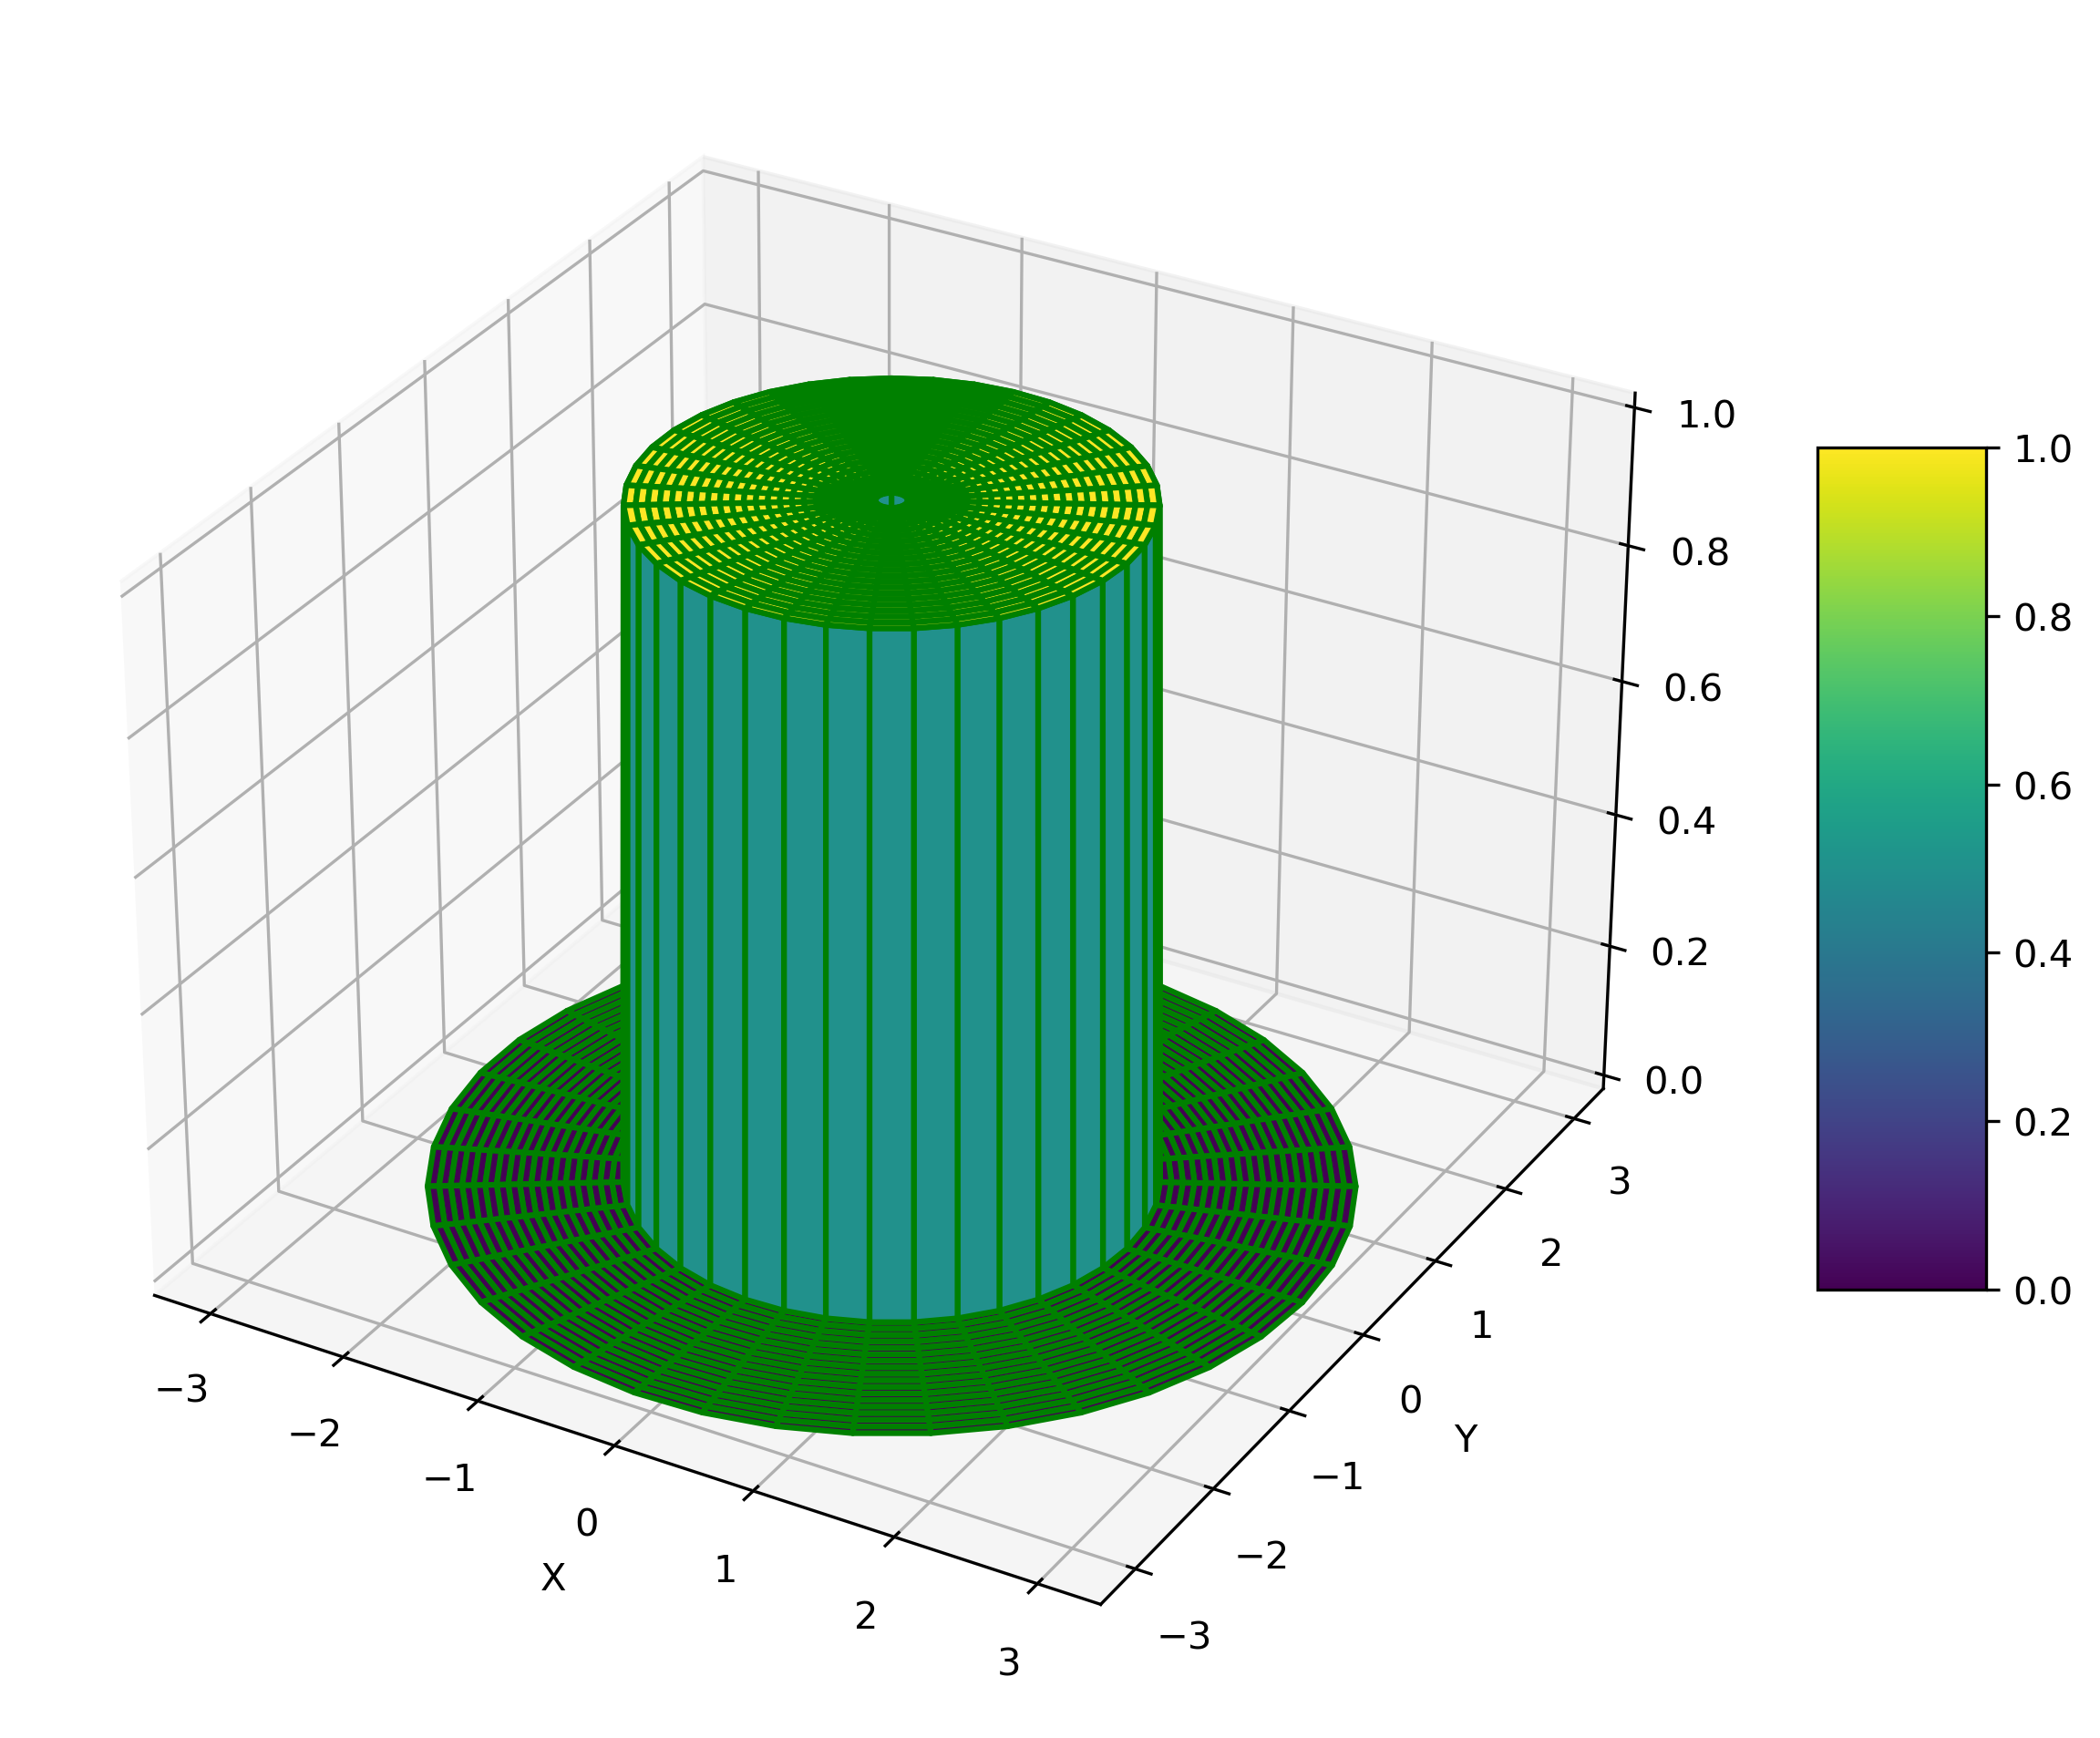
\includegraphics[width=\linewidth]{fig/psi_function_potential.png}
        \caption{$\Psi_{i}^l$関数のポテンシャル\Eqref{eq:psi_function}}
        \label{fig:psi_function_potential}
    \end{subfigure}
    
    \vspace{0.5cm}
    \begin{subfigure}[b]{0.45\linewidth}
        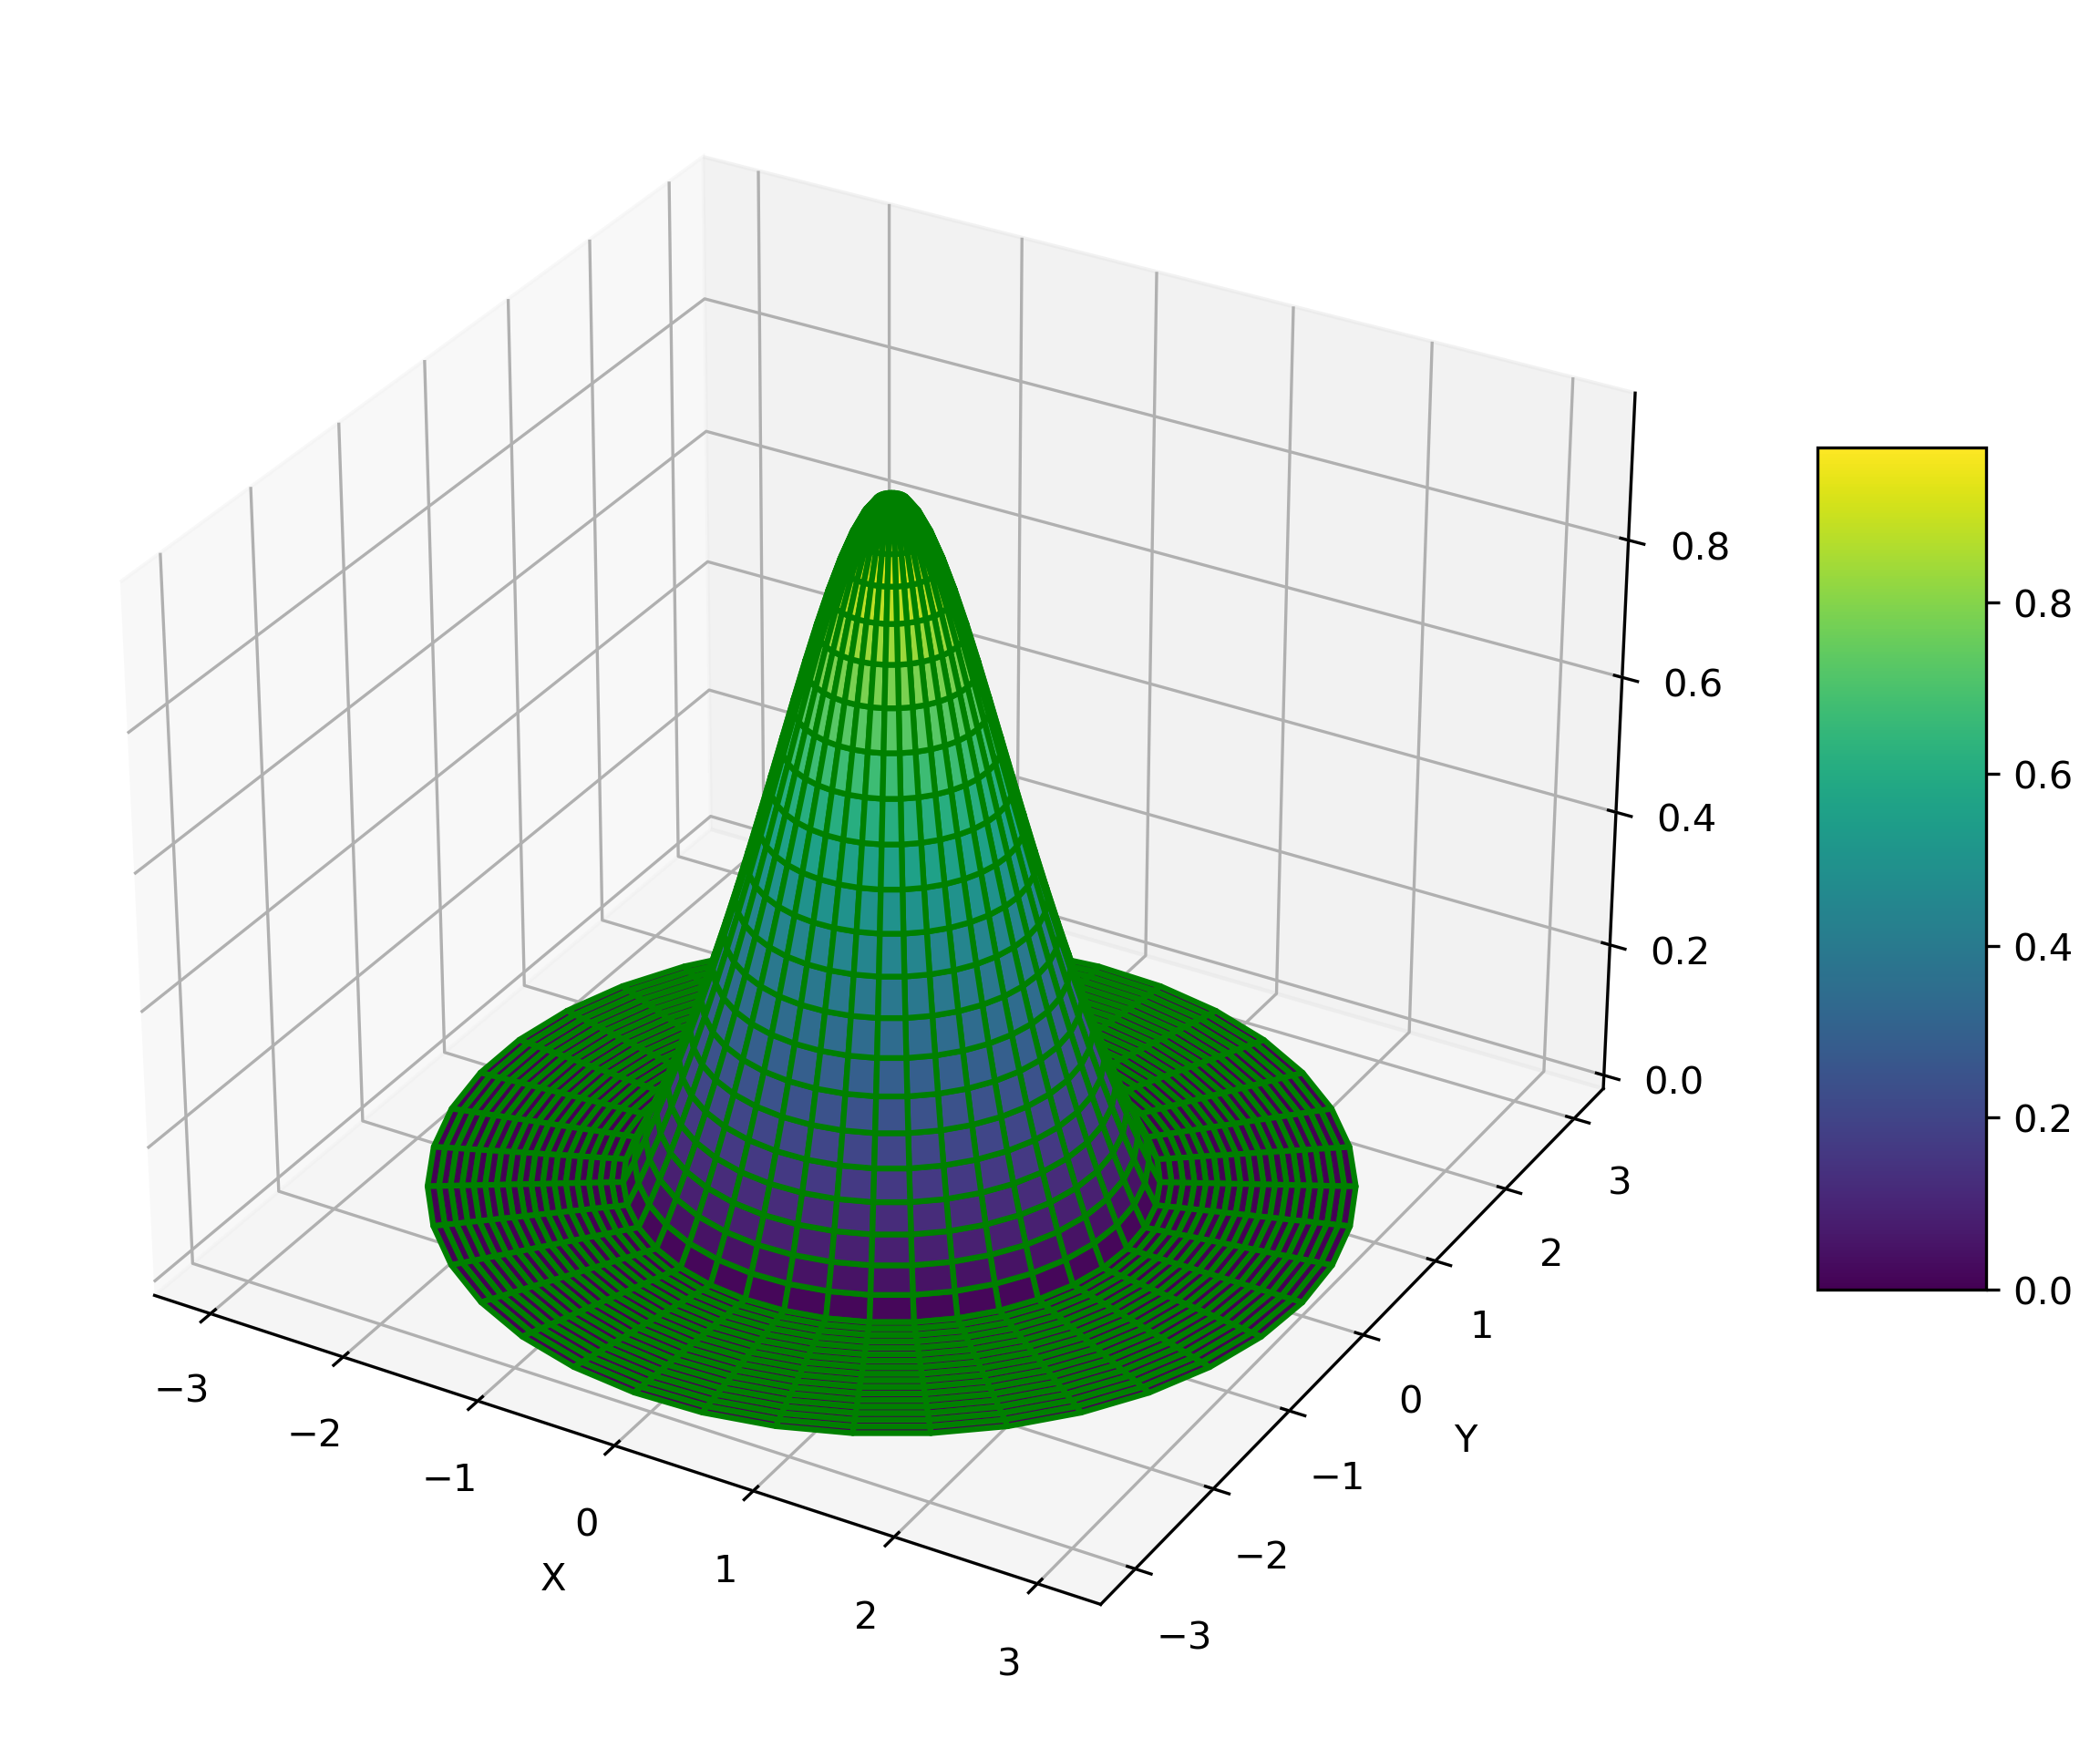
\includegraphics[width=\linewidth]{fig/p_function_potential.png}
        \caption{$P_i^l$関数のポテンシャル\Eqref{eq:new_probability_function}}
        \label{fig:p_function_potential}
    \end{subfigure}
    \hfill
    \begin{subfigure}[b]{0.45\linewidth}
        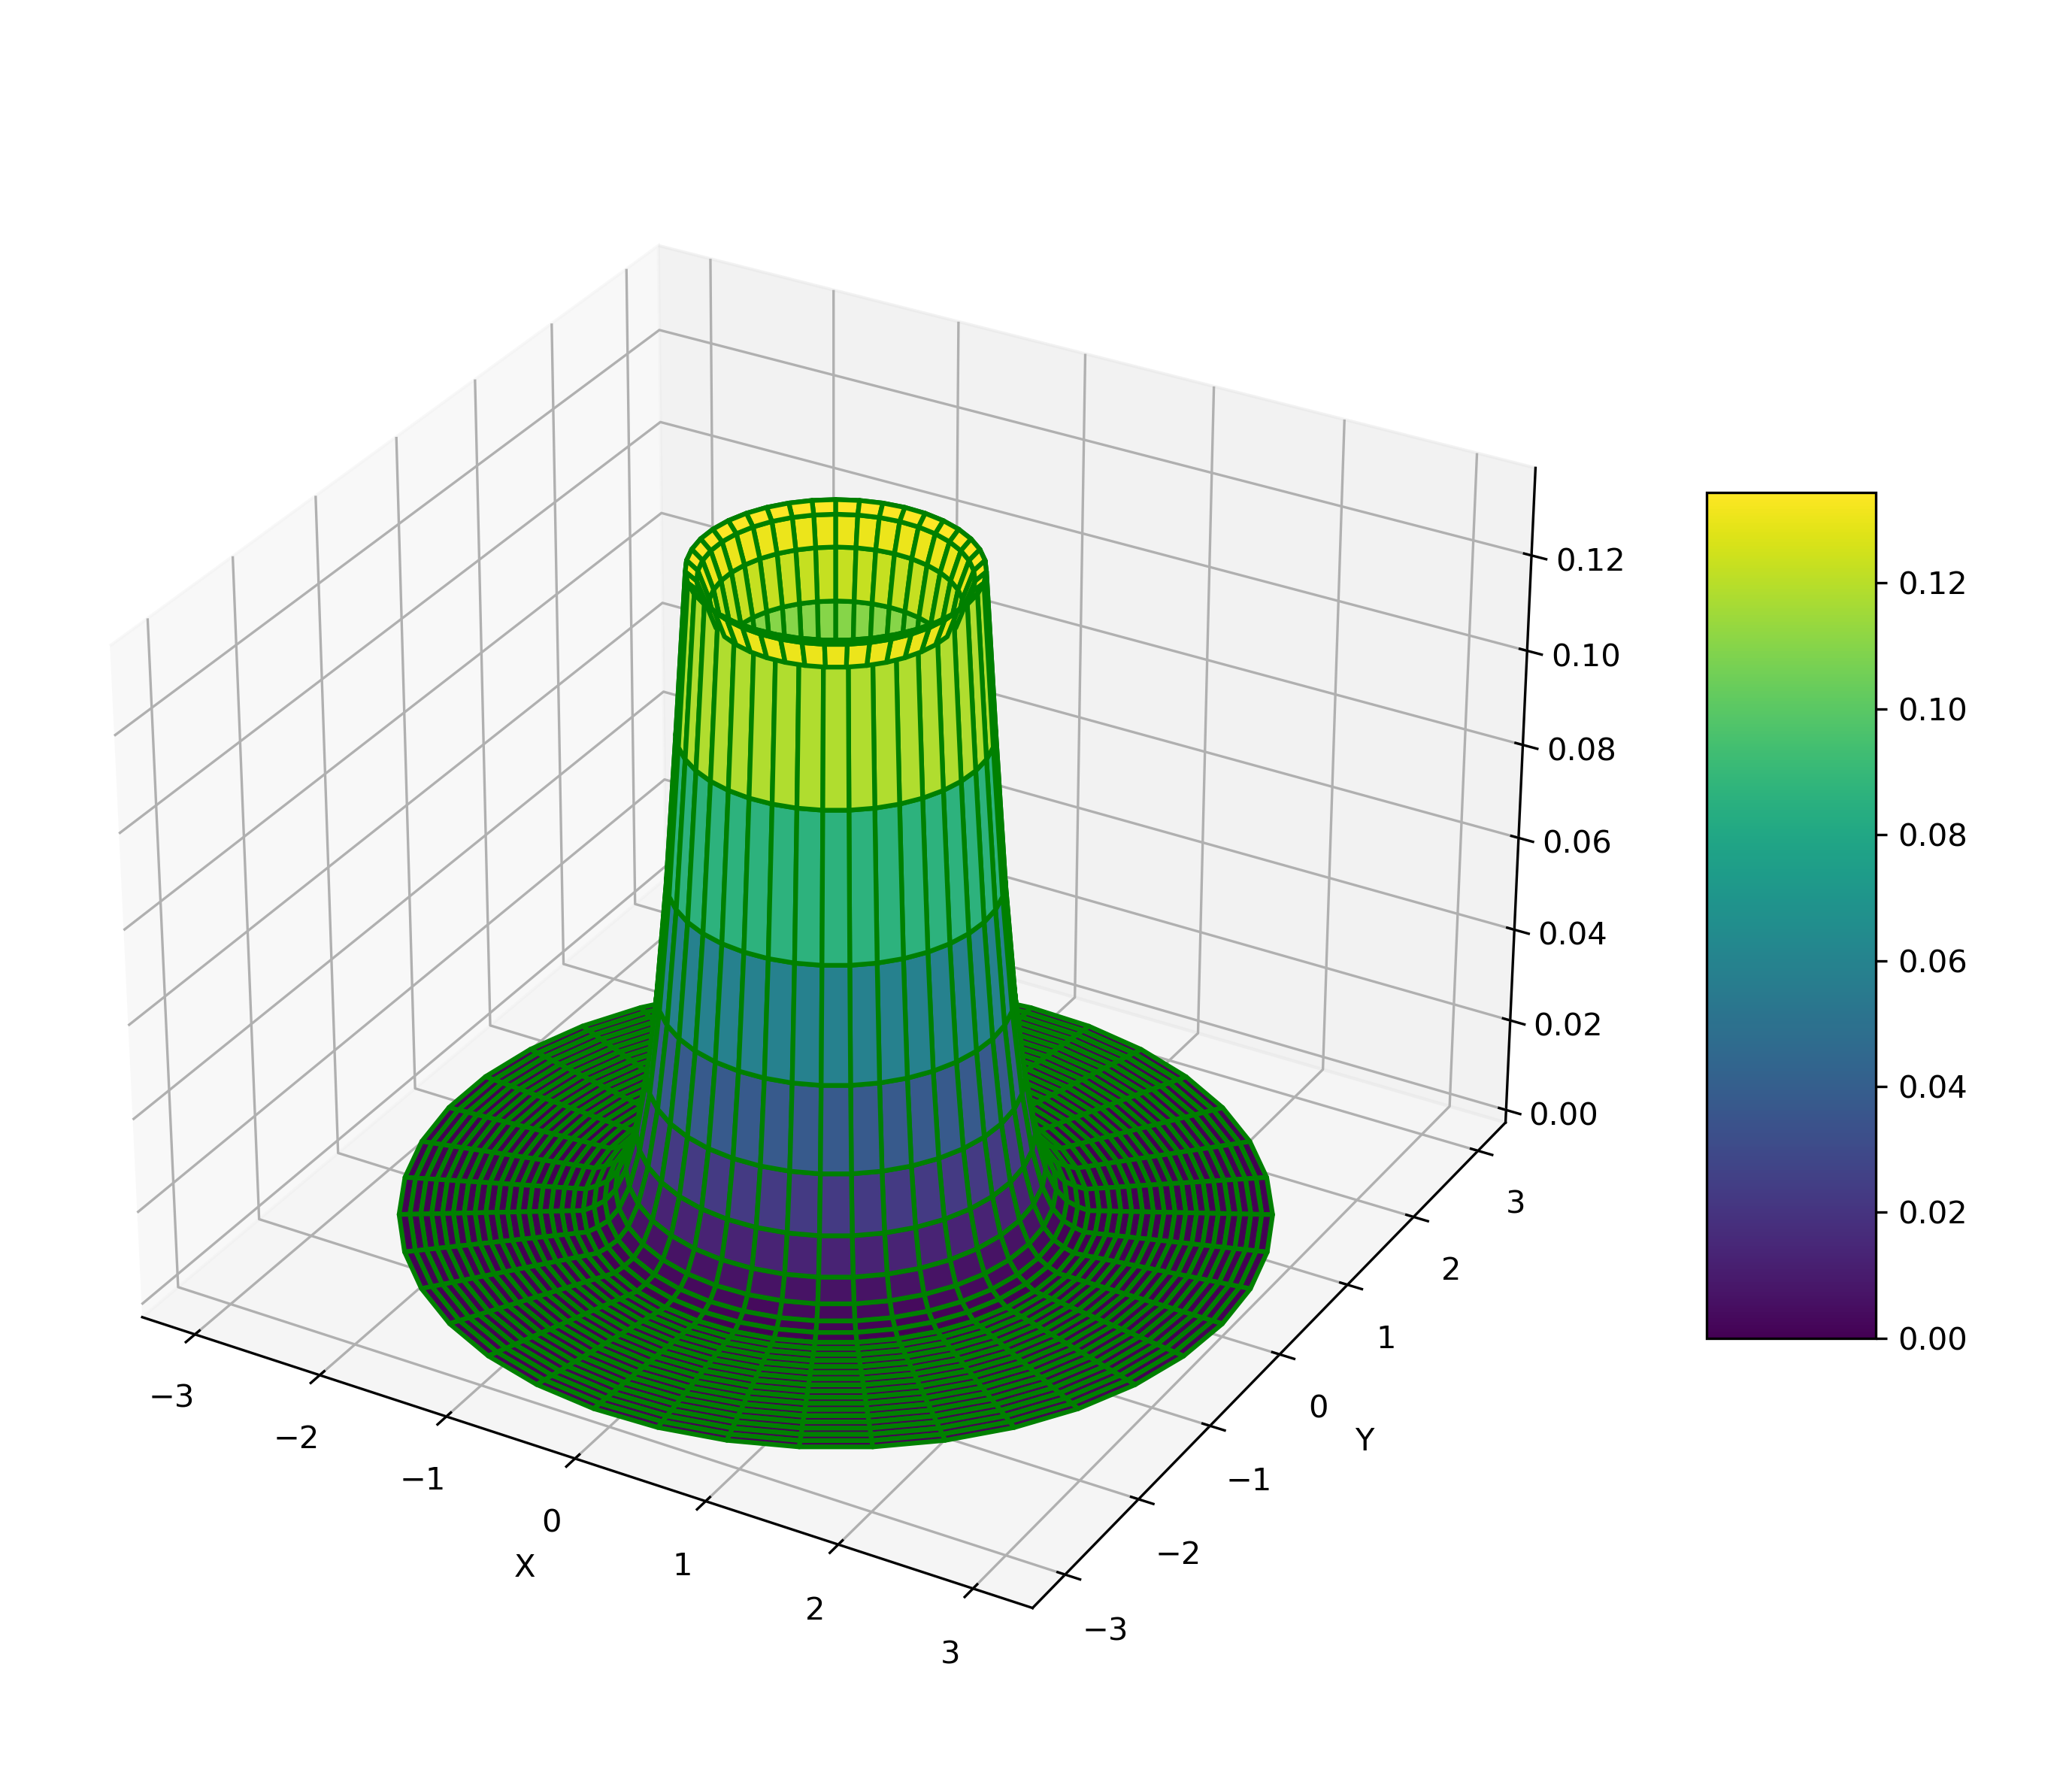
\includegraphics[width=\linewidth]{fig/covariance_function_potential.png}
        \caption{CRLB関数のポテンシャル\Eqref{eq:new_probability_function}}
        \label{fig:covariance_function_potential}
    \end{subfigure}
    \caption{確率関数のポテンシャル}
    \label{fig:potential_comparison}
\end{figure}

また,上記の検討から,\Eqref{eq:new_probability_function}によってCBFを設計する場合,\Figref{fig:CRLB}に示すように,CBFはクラメール・ラオの下限を上から抑える関数として機能することがわかる.クラメール・ラオの下限は最尤推定における最適化限界として働くため,理想的な推定アルゴリズムの元では,視野共有を保証するCBFは自己位置推定を行うためのアクティブパーセプションとして捉えることができる.
\begin{figure}[H]
    \centering
    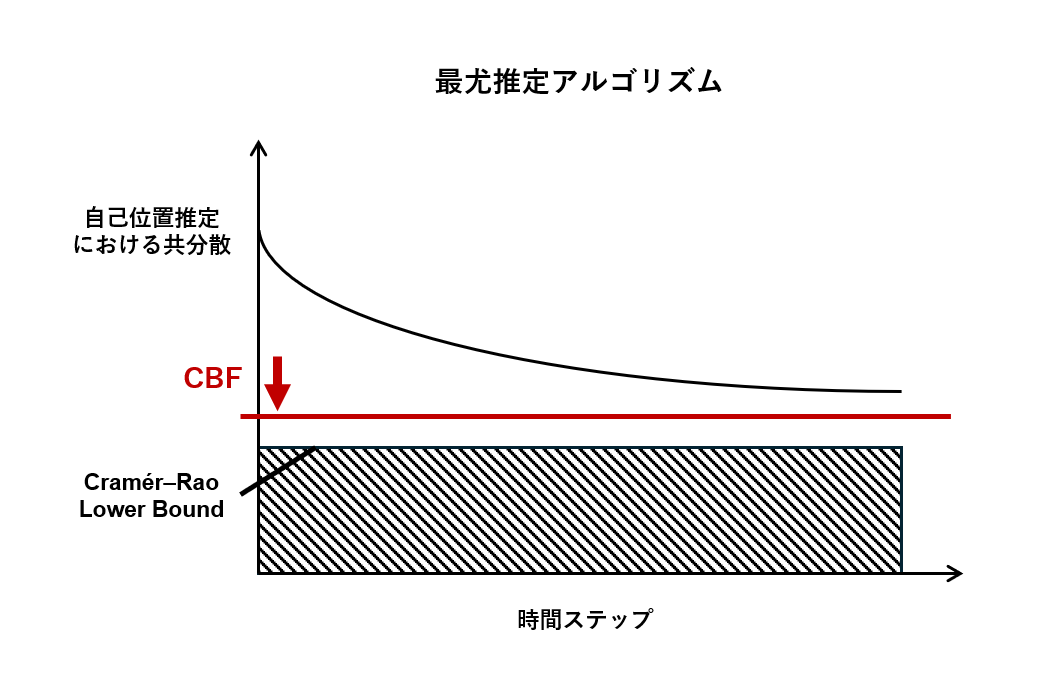
\includegraphics[width=0.7\linewidth]{fig/CRLB.png}
    \caption{クラメール・ラオの下限とCBFの関係}
    \label{fig:CRLB}
\end{figure}

\subsection{確率関数の時間微分と線形化}

確率関数をCBFに適用するには,確率関数の時間微分を制御入力$v_i, v_j$についての線形な関数に変換する必要がある.ここで
\begin{equation}
\begin{aligned}
\dot P_{ij}^l
&= -\frac{\sigma^2}{f^2}\,P_{ij}^l\,\dot T,\\
\dot T
&= \mathrm{tr}\left((M^{-1})^{\cdot}\right)
= -\mathrm{tr}\left(M^{-1}\dot M\,M^{-1}\right).
\end{aligned}
\label{eq:chain_rule}
\end{equation}

ただし$M$は各エージェント $k\in\{i,j\}$ の速度を $w_k=R_k v_k$ とし
\begin{equation}
\begin{aligned}
\dot M
&=\sum_{k\in\{i,j\}}
\frac{\mathrm d}{\mathrm dt}\left(\tfrac{P_{\beta_k}}{d_k^2}\right)\\
&=\sum_{k}
\frac{1}{d_k^2}\dot P_{\beta_k}
-\frac{2\dot d_k}{d_k^3}P_{\beta_k}\\
&=\sum_{k}
\frac{1}{d_k^3}\left[
P_{\beta_k}w_k\beta_k^\top
+\beta_k w_k^\top P_{\beta_k}
+2(\beta_k^\top w_k)P_{\beta_k}
\right].
\end{aligned}
\label{eq:Mdot}
\end{equation}
のように時間微分を計算することができる.

また,トレース演算は以下
\begin{equation}
\begin{aligned}
&\mathrm{tr}\left(M^{-1}\dot M\,M^{-1}\right)\\
&=\sum_{k\in\{i,j\}}
\frac{1}{d_k^3}\left[
\underbrace{\mathrm{tr}(M^{-1}P_{\beta_k}w_k\beta_k^\top M^{-1})}_{t_{k,1}}
+\underbrace{\mathrm{tr}(M^{-1}\beta_k w_k^\top P_{\beta_k}M^{-1})}_{t_{k,2}}
+\underbrace{2(\beta_k^\top w_k)\mathrm{tr}(M^{-1}P_{\beta_k}M^{-1})}_{t_{k,3}}
\right].
\end{aligned}
\label{eq:trace_expand}
\end{equation}
のように分解できる.ただし各項は
$\mathrm{tr}(A\,x\,y^\top\,B)=y^\top B A x$
により
\begin{equation}
\begin{aligned}
t_{k,1}&=w_k^\top P_{\beta_k}M^{-2}\beta_k,\\
t_{k,2}&=w_k^\top P_{\beta_k}M^{-2}\beta_k,\\
t_{k,3}&=2(\beta_k^\top w_k)\,\chi_k,\quad
\chi_k=\mathrm{tr}(M^{-1}P_{\beta_k}M^{-1}).
\end{aligned}
\label{eq:t_terms}
\end{equation}
を得る。よって
\begin{equation}
\begin{aligned}
\mathrm{tr}\left(M^{-1}\dot M\,M^{-1}\right)
&=\sum_{k}
\frac{2}{d_k^3}
w_k^\top\left(P_{\beta_k}M^{-2}\beta_k + \chi_k\beta_k\right).
\end{aligned}
\label{eq:trace_linear}
\end{equation}

上記の変形により,
\eqref{eq:chain_rule}, \eqref{eq:trace_linear} と $w_k=R_k v_k$ を組み合わせ,
\begin{equation}
\begin{aligned}
\dot P_{ij}^l
&=-\frac{\sigma^2}{f^2}P_{ij}^l\left(-\mathrm{tr}(M^{-1}\dot M\,M^{-1})\right)\\
&=\sum_{k\in\{i,j\}}
\lambda_k^\top v_k,
\end{aligned}
\label{eq:Pdot_prel}
\end{equation}
\[
\lambda_k
:=-\frac{2\sigma^2}{f^2}\,
\frac{P_{ij}^l}{d_k^3}\,
R_k^\top\left(P_{\beta_k}M^{-2}\beta_k + \chi_k\beta_k\right).
\]

最終的に
\begin{equation}
\begin{aligned}
\dot P_{ij}^l
= \lambda_i^\top v_i + \lambda_j^\top v_j
\end{aligned}
\label{eq:Pdot_linear}
\end{equation}
が得られる。以上で
$\dot P_{ij}^l$ がエージェント速度 $v_i,v_j$ に対し線形であることを示した。

今後の課題としては,今回シミュレーションを十分に検証できなかった2次系及び非ホロノミック系の結果検証の他,上記で示した自己位置推定における共分散を下限する確率関数の導入を行いたい.

\begin{thebibliography}{99}
\bibitem{Ames2017} A. D. Ames, X. Xu, J. W. Grizzle, and P. Tabuada, ``Control barrier function based quadratic programs for safety critical systems,'' {\it IEEE Transactions on Automatic Control}, Vol. 62, No. 8, pp. 3861-3876, 2017.

\bibitem{Arandjelovic2016} R. Arandjelovic, P. Gronat, A. Torii, T. Pajdla, and J. Sivic, ``NetVLAD: CNN architecture for weakly supervised place recognition,'' {\it Proceedings of the IEEE Conference on Computer Vision and Pattern Recognition}, pp. 5297-5307, 2016.

\bibitem{Capelli2020} B. Capelli and L. Sabattini, ``Connectivity maintenance: Global and optimized approach through control barrier functions,'' {\it Proceedings of the IEEE International Conference on Robotics and Automation (ICRA)}, pp. 5590-5596, 2020.

\bibitem{Chang2016} T.-H. Chang, M. Hong, W.-C. Liao, and X. Wang, ``Distributed optimization using the primal-dual method of multipliers,'' {\it IEEE Transactions on Signal Processing}, Vol. 64, No. 2, pp. 447-461, 2016.

\bibitem{DeTone2018} D. DeTone, T. Malisiewicz, and A. Rabinovich, ``SuperPoint: Self-supervised interest point detection and description,'' {\it Proceedings of the IEEE Conference on Computer Vision and Pattern Recognition Workshops}, pp. 224-236, 2018.

\bibitem{Dias2016} D. Dias, P. U. Lima, and A. Martinoli, ``Distributed Formation Control of Quadrotors under Limited Sensor Field of View,'' {\it Proceedings of the International Conference on Autonomous Agents and Multiagent Systems (AAMAS)}, pp. 1087-1095, 2016.

\bibitem{Jankovic2022} M. Jankovic, M. Egerstedt, and S. Coogan, ``Barrier functions for multiagent systems: An overview,'' {\it Annual Reviews in Control}, Vol. 53, pp. 329-348, 2022.

\bibitem{Lee2010} T. Lee, M. Leok, and N. H. McClamroch, ``Geometric tracking control of a quadrotor UAV on SE(3),'' {\it Proceedings of the IEEE Conference on Decision and Control}, pp. 5420-5425, 2010.

\bibitem{Lee2013} T. Lee, M. Leok, and N. H. McClamroch, ``Nonlinear robust tracking control of a quadrotor UAV on SE(3),'' {\it Asian Journal of Control}, Vol. 15, No. 2, pp. 391-408, 2013.

\bibitem{Lv2024} X. Lv, C. Peng, and J. Ma, ``Control Barrier Function-Based Collision Avoidance Guidance Strategy for Multi-Fixed-Wing UAV Pursuit-Evasion Environment,'' {\it Drones}, Vol. 8, No. 8, pp. 415, 2024.

\bibitem{Panagou2012} D. Panagou and V. Kumar, ``Maintaining visibility for leader-follower formations in obstacle environments,'' {\it Proceedings of the IEEE International Conference on Robotics and Automation (ICRA)}, pp. 1811-1816, 2012.

\bibitem{Panagou2017} D. Panagou, D. M. Stipanovic, and P. G. Voulgaris, ``Distributed dynamic coverage and avoidance control under anisotropic sensing,'' {\it IEEE Transactions on Control of Network Systems}, Vol. 4, No. 4, pp. 850-862, 2017.

\bibitem{Sabattini2013} L. Sabattini, C. Secchi, and N. Chopra, ``Decentralized control for the maintenance of strong connectivity for directed graphs,'' {\it Proceedings of the Mediterranean Conference on Control and Automation}, pp. 978-986, 2013.

\bibitem{Zhang2022} T. Zhang, L. Zhang, Y. Chen, and Y. Zhou, ``CVIDS: A collaborative localization and dense mapping framework for multi-agent based visual-inertial SLAM,'' {\it IEEE Transactions on Image Processing}, Vol. 31, pp. 6562-6576, 2022.

\bibitem{Tan2022} X. Tan and D. V. Dimarogonas, ``Distributed Implementation of Control Barrier Functions for Multi-agent Systems,'' {\it IEEE Control Systems Letters}, Vol. 6, pp. 1879-1884, 2022.

\bibitem{Taylor2020} A. J. Taylor, A. Singletary, Y. Yue, and A. D. Ames, ``Learning for safety-critical control with control barrier functions,'' {\it Proceedings of the 2nd Conference on Learning for Dynamics and Control}, pp. 708-717, 2020.

\bibitem{Trimarchi2025} B. Trimarchi, F. Schiano, and R. Tron, ``A Control Barrier Function Candidate for Quadrotors with Limited Field of View,'' {\it arXiv:2410.01277 [eess.SY]}, 2025.

\bibitem{Wang2017} Y. Wang, A. D. Ames, and M. Egerstedt, ``Safety barrier certificates for collisions-free multi-robot systems,'' {\it IEEE Transactions on Robotics}, Vol. 33, No. 3, pp. 641-652, 2017.

\bibitem{Xiao2022} W. Xiao and C. Belta, ``High-order control barrier functions,'' {\it IEEE Transactions on Automatic Control}, Vol. 67, No. 7, pp. 3655-3662, 2022.

\bibitem{Zhang2017} G. Zhang and R. Heusdens, ``Distributed Optimization Using the Primal-Dual Method of Multipliers (PDMM),'' {\it arXiv:1702.00841 [cs.DC]}, 2017.


\bibitem{Zhang2018} Z. Zhang and D. Scaramuzza, ``Perception-aware receding horizon navigation for MAVs,'' {\it Proceedings of the IEEE International Conference on Robotics and Automation (ICRA)}, pp. 2534-2541, 2018.
\end{thebibliography}


%\processdelayedfloats %%% See above for an explanation of why this command might be needed here.


\end{document}
